%********************************************%
%*       Generated from PreTeXt source      *%
%*       on 2023-02-03T09:04:17-05:00       *%
%*   A recent stable commit (2022-07-01):   *%
%* 6c761d3dba23af92cba35001c852aac04ae99a5f *%
%*                                          *%
%*         https://pretextbook.org          *%
%*                                          *%
%********************************************%
\documentclass[oneside,10pt,]{book}
%% Custom Preamble Entries, early (use latex.preamble.early)
%% Default LaTeX packages
%%   1.  always employed (or nearly so) for some purpose, or
%%   2.  a stylewriter may assume their presence
\usepackage{geometry}
%% Some aspects of the preamble are conditional,
%% the LaTeX engine is one such determinant
\usepackage{ifthen}
%% etoolbox has a variety of modern conveniences
\usepackage{etoolbox}
\usepackage{ifxetex,ifluatex}
%% Raster graphics inclusion
\usepackage{graphicx}
%% Color support, xcolor package
%% Always loaded, for: add/delete text, author tools
%% Here, since tcolorbox loads tikz, and tikz loads xcolor
\PassOptionsToPackage{usenames,dvipsnames,svgnames,table}{xcolor}
\usepackage{xcolor}
%% begin: defined colors, via xcolor package, for styling
%% end: defined colors, via xcolor package, for styling
%% Colored boxes, and much more, though mostly styling
%% skins library provides "enhanced" skin, employing tikzpicture
%% boxes may be configured as "breakable" or "unbreakable"
%% "raster" controls grids of boxes, aka side-by-side
\usepackage{tcolorbox}
\tcbuselibrary{skins}
\tcbuselibrary{breakable}
\tcbuselibrary{raster}
%% We load some "stock" tcolorbox styles that we use a lot
%% Placement here is provisional, there will be some color work also
%% First, black on white, no border, transparent, but no assumption about titles
\tcbset{ bwminimalstyle/.style={size=minimal, boxrule=-0.3pt, frame empty,
colback=white, colbacktitle=white, coltitle=black, opacityfill=0.0} }
%% Second, bold title, run-in to text/paragraph/heading
%% Space afterwards will be controlled by environment,
%% independent of constructions of the tcb title
%% Places \blocktitlefont onto many block titles
\tcbset{ runintitlestyle/.style={fonttitle=\blocktitlefont\upshape\bfseries, attach title to upper} }
%% Spacing prior to each exercise, anywhere
\tcbset{ exercisespacingstyle/.style={before skip={1.5ex plus 0.5ex}} }
%% Spacing prior to each block
\tcbset{ blockspacingstyle/.style={before skip={2.0ex plus 0.5ex}} }
%% xparse allows the construction of more robust commands,
%% this is a necessity for isolating styling and behavior
%% The tcolorbox library of the same name loads the base library
\tcbuselibrary{xparse}
%% The tcolorbox library loads TikZ, its calc package is generally useful,
%% and is necessary for some smaller documents that use partial tcolor boxes
%% See:  https://github.com/PreTeXtBook/pretext/issues/1624
\usetikzlibrary{calc}
%% Hyperref should be here, but likes to be loaded late
%%
%% Inline math delimiters, \(, \), need to be robust
%% 2016-01-31:  latexrelease.sty  supersedes  fixltx2e.sty
%% If  latexrelease.sty  exists, bugfix is in kernel
%% If not, bugfix is in  fixltx2e.sty
%% See:  https://tug.org/TUGboat/tb36-3/tb114ltnews22.pdf
%% and read "Fewer fragile commands" in distribution's  latexchanges.pdf
\IfFileExists{latexrelease.sty}{}{\usepackage{fixltx2e}}
%% shorter subnumbers in some side-by-side require manipulations
\usepackage{xstring}
%% Text height identically 9 inches, text width varies on point size
%% See Bringhurst 2.1.1 on measure for recommendations
%% 75 characters per line (count spaces, punctuation) is target
%% which is the upper limit of Bringhurst's recommendations
\geometry{letterpaper,total={340pt,9.0in}}
%% Custom Page Layout Adjustments (use publisher page-geometry entry)
%% This LaTeX file may be compiled with pdflatex, xelatex, or lualatex executables
%% LuaTeX is not explicitly supported, but we do accept additions from knowledgeable users
%% The conditional below provides  pdflatex  specific configuration last
%% begin: engine-specific capabilities
\ifthenelse{\boolean{xetex} \or \boolean{luatex}}{%
%% begin: xelatex and lualatex-specific default configuration
\ifxetex\usepackage{xltxtra}\fi
%% realscripts is the only part of xltxtra relevant to lualatex 
\ifluatex\usepackage{realscripts}\fi
%% end:   xelatex and lualatex-specific default configuration
}{
%% begin: pdflatex-specific default configuration
%% We assume a PreTeXt XML source file may have Unicode characters
%% and so we ask LaTeX to parse a UTF-8 encoded file
%% This may work well for accented characters in Western language,
%% but not with Greek, Asian languages, etc.
%% When this is not good enough, switch to the  xelatex  engine
%% where Unicode is better supported (encouraged, even)
\usepackage[utf8]{inputenc}
%% end: pdflatex-specific default configuration
}
%% end:   engine-specific capabilities
%%
%% Fonts.  Conditional on LaTex engine employed.
%% Default Text Font: The Latin Modern fonts are
%% "enhanced versions of the [original TeX] Computer Modern fonts."
%% We use them as the default text font for PreTeXt output.
%% Default Monospace font: Inconsolata (aka zi4)
%% Sponsored by TUG: http://levien.com/type/myfonts/inconsolata.html
%% Loaded for documents with intentional objects requiring monospace
%% See package documentation for excellent instructions
%% fontspec will work universally if we use filename to locate OTF files
%% Loads the "upquote" package as needed, so we don't have to
%% Upright quotes might come from the  textcomp  package, which we also use
%% We employ the shapely \ell to match Google Font version
%% pdflatex: "varl" package option produces shapely \ell
%% pdflatex: "var0" package option produces plain zero (not used)
%% pdflatex: "varqu" package option produces best upright quotes
%% xelatex,lualatex: add OTF StylisticSet 1 for shapely \ell
%% xelatex,lualatex: add OTF StylisticSet 2 for plain zero (not used)
%% xelatex,lualatex: add OTF StylisticSet 3 for upright quotes
%%
%% Automatic Font Control
%% Portions of a document, are, or may, be affected by defined commands
%% These are perhaps more flexible when using  xelatex  rather than  pdflatex
%% The following definitions are meant to be re-defined in a style, using \renewcommand
%% They are scoped when employed (in a TeX group), and so should not be defined with an argument
\newcommand{\divisionfont}{\relax}
\newcommand{\blocktitlefont}{\relax}
\newcommand{\contentsfont}{\relax}
\newcommand{\pagefont}{\relax}
\newcommand{\tabularfont}{\relax}
\newcommand{\xreffont}{\relax}
\newcommand{\titlepagefont}{\relax}
%%
\ifthenelse{\boolean{xetex} \or \boolean{luatex}}{%
%% begin: font setup and configuration for use with xelatex
%% Generally, xelatex is necessary for non-Western fonts
%% fontspec package provides extensive control of system fonts,
%% meaning *.otf (OpenType), and apparently *.ttf (TrueType)
%% that live *outside* your TeX/MF tree, and are controlled by your *system*
%% (it is possible that a TeX distribution will place fonts in a system location)
%%
%% The fontspec package is the best vehicle for using different fonts in  xelatex
%% So we load it always, no matter what a publisher or style might want
%%
\usepackage{fontspec}
%%
%% begin: xelatex main font ("font-xelatex-main" template)
%% Latin Modern Roman is the default font for xelatex and so is loaded with a TU encoding
%% *in the format* so we can't touch it, only perhaps adjust it later
%% in one of two ways (then known by NFSS names such as "lmr")
%% (1) via NFSS with font family names such as "lmr" and "lmss"
%% (2) via fontspec with commands like \setmainfont{Latin Modern Roman}
%% The latter requires the font to be known at the system-level by its font name,
%% but will give access to OTF font features through optional arguments
%% https://tex.stackexchange.com/questions/470008/
%% where-and-how-does-fontspec-sty-specify-the-default-font-latin-modern-roman
%% http://tex.stackexchange.com/questions/115321
%% /how-to-optimize-latin-modern-font-with-xelatex
%%
%% end:   xelatex main font ("font-xelatex-main" template)
%% begin: xelatex mono font ("font-xelatex-mono" template)
%% (conditional on non-trivial uses being present in source)
\IfFontExistsTF{Inconsolatazi4-Regular.otf}{}{\GenericError{}{The font "Inconsolatazi4-Regular.otf" requested by PreTeXt output is not available.  Either a file cannot be located in default locations via a filename, or a font is not known by its name as part of your system.}{Consult the PreTeXt Guide for help with LaTeX fonts.}{}}
\IfFontExistsTF{Inconsolatazi4-Bold.otf}{}{\GenericError{}{The font "Inconsolatazi4-Bold.otf" requested by PreTeXt output is not available.  Either a file cannot be located in default locations via a filename, or a font is not known by its name as part of your system.}{Consult the PreTeXt Guide for help with LaTeX fonts.}{}}
\usepackage{zi4}
\setmonofont[BoldFont=Inconsolatazi4-Bold.otf,StylisticSet={1,3}]{Inconsolatazi4-Regular.otf}
%% end:   xelatex mono font ("font-xelatex-mono" template)
%% begin: xelatex font adjustments ("font-xelatex-style" template)
%% end:   xelatex font adjustments ("font-xelatex-style" template)
%%
%% Extensive support for other languages
\usepackage{polyglossia}
%% Set main/default language based on pretext/@xml:lang value
%% document language code is "en-US", US English
%% usmax variant has extra hypenation
\setmainlanguage[variant=usmax]{english}
%% Enable secondary languages based on discovery of @xml:lang values
%% Enable fonts/scripts based on discovery of @xml:lang values
%% Western languages should be ably covered by Latin Modern Roman
%% end:   font setup and configuration for use with xelatex
}{%
%% begin: font setup and configuration for use with pdflatex
%% begin: pdflatex main font ("font-pdflatex-main" template)
\usepackage{lmodern}
\usepackage[T1]{fontenc}
%% end:   pdflatex main font ("font-pdflatex-main" template)
%% begin: pdflatex mono font ("font-pdflatex-mono" template)
%% (conditional on non-trivial uses being present in source)
\usepackage[varqu,varl]{inconsolata}
%% end:   pdflatex mono font ("font-pdflatex-mono" template)
%% begin: pdflatex font adjustments ("font-pdflatex-style" template)
%% end:   pdflatex font adjustments ("font-pdflatex-style" template)
%% end:   font setup and configuration for use with pdflatex
}
%% Micromanage spacing, etc.  The named "microtype-options"
%% template may be employed to fine-tune package behavior
\usepackage{microtype}
%% Symbols, align environment, commutative diagrams, bracket-matrix
\usepackage{amsmath}
\usepackage{amscd}
\usepackage{amssymb}
%% allow page breaks within display mathematics anywhere
%% level 4 is maximally permissive
%% this is exactly the opposite of AMSmath package philosophy
%% there are per-display, and per-equation options to control this
%% split, aligned, gathered, and alignedat are not affected
\allowdisplaybreaks[4]
%% allow more columns to a matrix
%% can make this even bigger by overriding with  latex.preamble.late  processing option
\setcounter{MaxMatrixCols}{30}
%%
%%
%% Division Titles, and Page Headers/Footers
%% titlesec package, loading "titleps" package cooperatively
%% See code comments about the necessity and purpose of "explicit" option.
%% The "newparttoc" option causes a consistent entry for parts in the ToC 
%% file, but it is only effective if there is a \titleformat for \part.
%% "pagestyles" loads the  titleps  package cooperatively.
\usepackage[explicit, newparttoc, pagestyles]{titlesec}
%% The companion titletoc package for the ToC.
\usepackage{titletoc}
%% Fixes a bug with transition from chapters to appendices in a "book"
%% See generating XSL code for more details about necessity
\newtitlemark{\chaptertitlename}
%% begin: customizations of page styles via the modal "titleps-style" template
%% Designed to use commands from the LaTeX "titleps" package
%% Plain pages should have the same font for page numbers
\renewpagestyle{plain}{%
\setfoot{}{\pagefont\thepage}{}%
}%
%% Single pages as in default LaTeX
\renewpagestyle{headings}{%
\sethead{\pagefont\slshape\MakeUppercase{\ifthechapter{\chaptertitlename\space\thechapter.\space}{}\chaptertitle}}{}{\pagefont\thepage}%
}%
\pagestyle{headings}
%% end: customizations of page styles via the modal "titleps-style" template
%%
%% Create globally-available macros to be provided for style writers
%% These are redefined for each occurence of each division
\newcommand{\divisionnameptx}{\relax}%
\newcommand{\titleptx}{\relax}%
\newcommand{\subtitleptx}{\relax}%
\newcommand{\shortitleptx}{\relax}%
\newcommand{\authorsptx}{\relax}%
\newcommand{\epigraphptx}{\relax}%
%% Create environments for possible occurences of each division
%% Environment for a PTX "preface" at the level of a LaTeX "chapter"
\NewDocumentEnvironment{preface}{mmmmmmm}
{%
\renewcommand{\divisionnameptx}{#1}%
\renewcommand{\titleptx}{#2}%
\renewcommand{\subtitleptx}{#3}%
\renewcommand{\shortitleptx}{#4}%
\renewcommand{\authorsptx}{#5}%
\renewcommand{\epigraphptx}{#6}%
\chapter*{#2}%
\addcontentsline{toc}{chapter}{#4}
\label{#7}%
}{}%
%% Environment for a PTX "chapter" at the level of a LaTeX "chapter"
\NewDocumentEnvironment{chapterptx}{mmmmmmm}
{%
\renewcommand{\divisionnameptx}{#1}%
\renewcommand{\titleptx}{#2}%
\renewcommand{\subtitleptx}{#3}%
\renewcommand{\shortitleptx}{#4}%
\renewcommand{\authorsptx}{#5}%
\renewcommand{\epigraphptx}{#6}%
\chapter[{#4}]{#2}%
\label{#7}%
}{}%
%% Environment for a PTX "section" at the level of a LaTeX "section"
\NewDocumentEnvironment{sectionptx}{mmmmmmm}
{%
\renewcommand{\divisionnameptx}{#1}%
\renewcommand{\titleptx}{#2}%
\renewcommand{\subtitleptx}{#3}%
\renewcommand{\shortitleptx}{#4}%
\renewcommand{\authorsptx}{#5}%
\renewcommand{\epigraphptx}{#6}%
\section[{#4}]{#2}%
\label{#7}%
}{}%
%% Environment for a PTX "exercises" at the level of a LaTeX "section"
\NewDocumentEnvironment{exercises-section}{mmmmmmm}
{%
\renewcommand{\divisionnameptx}{#1}%
\renewcommand{\titleptx}{#2}%
\renewcommand{\subtitleptx}{#3}%
\renewcommand{\shortitleptx}{#4}%
\renewcommand{\authorsptx}{#5}%
\renewcommand{\epigraphptx}{#6}%
\section[{#4}]{#2}%
\label{#7}%
}{}%
%% Environment for a PTX "exercises" at the level of a LaTeX "section"
\NewDocumentEnvironment{exercises-section-numberless}{mmmmmmm}
{%
\renewcommand{\divisionnameptx}{#1}%
\renewcommand{\titleptx}{#2}%
\renewcommand{\subtitleptx}{#3}%
\renewcommand{\shortitleptx}{#4}%
\renewcommand{\authorsptx}{#5}%
\renewcommand{\epigraphptx}{#6}%
\section*{#2}%
\addcontentsline{toc}{section}{#4}
\label{#7}%
}{}%
%% Environment for a PTX "appendix" at the level of a LaTeX "chapter"
\NewDocumentEnvironment{appendixptx}{mmmmmmm}
{%
\renewcommand{\divisionnameptx}{#1}%
\renewcommand{\titleptx}{#2}%
\renewcommand{\subtitleptx}{#3}%
\renewcommand{\shortitleptx}{#4}%
\renewcommand{\authorsptx}{#5}%
\renewcommand{\epigraphptx}{#6}%
\chapter[{#4}]{#2}%
\label{#7}%
}{}%
%% Environment for a PTX "references" at the level of a LaTeX "chapter"
\NewDocumentEnvironment{references-chapter}{mmmmmmm}
{%
\renewcommand{\divisionnameptx}{#1}%
\renewcommand{\titleptx}{#2}%
\renewcommand{\subtitleptx}{#3}%
\renewcommand{\shortitleptx}{#4}%
\renewcommand{\authorsptx}{#5}%
\renewcommand{\epigraphptx}{#6}%
\chapter[{#4}]{#2}%
\label{#7}%
}{}%
%% Environment for a PTX "references" at the level of a LaTeX "chapter"
\NewDocumentEnvironment{references-chapter-numberless}{mmmmmmm}
{%
\renewcommand{\divisionnameptx}{#1}%
\renewcommand{\titleptx}{#2}%
\renewcommand{\subtitleptx}{#3}%
\renewcommand{\shortitleptx}{#4}%
\renewcommand{\authorsptx}{#5}%
\renewcommand{\epigraphptx}{#6}%
\chapter*{#2}%
\addcontentsline{toc}{chapter}{#4}
\label{#7}%
}{}%
%% Environment for a PTX "index" at the level of a LaTeX "chapter"
\NewDocumentEnvironment{indexptx}{mmmmmmm}
{%
\renewcommand{\divisionnameptx}{#1}%
\renewcommand{\titleptx}{#2}%
\renewcommand{\subtitleptx}{#3}%
\renewcommand{\shortitleptx}{#4}%
\renewcommand{\authorsptx}{#5}%
\renewcommand{\epigraphptx}{#6}%
\chapter*{#2}%
\addcontentsline{toc}{chapter}{#4}
\label{#7}%
}{}%
%%
%% Styles for six traditional LaTeX divisions
\titleformat{\part}[display]
{\divisionfont\Huge\bfseries\centering}{\divisionnameptx\space\thepart}{30pt}{\Huge#1}
[{\Large\centering\authorsptx}]
\titleformat{\chapter}[display]
{\divisionfont\huge\bfseries}{\divisionnameptx\space\thechapter}{20pt}{\Huge#1}
[{\Large\authorsptx}]
\titleformat{name=\chapter,numberless}[display]
{\divisionfont\huge\bfseries}{}{0pt}{#1}
[{\Large\authorsptx}]
\titlespacing*{\chapter}{0pt}{50pt}{40pt}
\titleformat{\section}[hang]
{\divisionfont\Large\bfseries}{\thesection}{1ex}{#1}
[{\large\authorsptx}]
\titleformat{name=\section,numberless}[block]
{\divisionfont\Large\bfseries}{}{0pt}{#1}
[{\large\authorsptx}]
\titlespacing*{\section}{0pt}{3.5ex plus 1ex minus .2ex}{2.3ex plus .2ex}
\titleformat{\subsection}[hang]
{\divisionfont\large\bfseries}{\thesubsection}{1ex}{#1}
[{\normalsize\authorsptx}]
\titleformat{name=\subsection,numberless}[block]
{\divisionfont\large\bfseries}{}{0pt}{#1}
[{\normalsize\authorsptx}]
\titlespacing*{\subsection}{0pt}{3.25ex plus 1ex minus .2ex}{1.5ex plus .2ex}
\titleformat{\subsubsection}[hang]
{\divisionfont\normalsize\bfseries}{\thesubsubsection}{1em}{#1}
[{\small\authorsptx}]
\titleformat{name=\subsubsection,numberless}[block]
{\divisionfont\normalsize\bfseries}{}{0pt}{#1}
[{\normalsize\authorsptx}]
\titlespacing*{\subsubsection}{0pt}{3.25ex plus 1ex minus .2ex}{1.5ex plus .2ex}
\titleformat{\paragraph}[hang]
{\divisionfont\normalsize\bfseries}{\theparagraph}{1em}{#1}
[{\small\authorsptx}]
\titleformat{name=\paragraph,numberless}[block]
{\divisionfont\normalsize\bfseries}{}{0pt}{#1}
[{\normalsize\authorsptx}]
\titlespacing*{\paragraph}{0pt}{3.25ex plus 1ex minus .2ex}{1.5em}
%%
%% Styles for five traditional LaTeX divisions
\titlecontents{part}%
[0pt]{\contentsmargin{0em}\addvspace{1pc}\contentsfont\bfseries}%
{\Large\thecontentslabel\enspace}{\Large}%
{}%
[\addvspace{.5pc}]%
\titlecontents{chapter}%
[0pt]{\contentsmargin{0em}\addvspace{1pc}\contentsfont\bfseries}%
{\large\thecontentslabel\enspace}{\large}%
{\hfill\bfseries\thecontentspage}%
[\addvspace{.5pc}]%
\dottedcontents{section}[3.8em]{\contentsfont}{2.3em}{1pc}%
\dottedcontents{subsection}[6.1em]{\contentsfont}{3.2em}{1pc}%
\dottedcontents{subsubsection}[9.3em]{\contentsfont}{4.3em}{1pc}%
%%
%% Begin: Semantic Macros
%% To preserve meaning in a LaTeX file
%%
%% \mono macro for content of "c", "cd", "tag", etc elements
%% Also used automatically in other constructions
%% Simply an alias for \texttt
%% Always defined, even if there is no need, or if a specific tt font is not loaded
\newcommand{\mono}[1]{\texttt{#1}}
%%
%% Following semantic macros are only defined here if their
%% use is required only in this specific document
%%
%% Used for inline definitions of terms
\newcommand{\terminology}[1]{\textbf{#1}}
%% End: Semantic Macros
%% Divisional exercises (and worksheet) as LaTeX environments
%% Third argument is option for extra workspace in worksheets
%% Hanging indent occupies a 5ex width slot prior to left margin
%% Experimentally this seems just barely sufficient for a bold "888."
%% Division exercises, not in exercise group
\tcbset{ divisionexercisestyle/.style={bwminimalstyle, runintitlestyle, exercisespacingstyle, left=5ex, breakable, parbox=false } }
\newtcolorbox{divisionexercise}[4]{divisionexercisestyle, before title={\hspace{-5ex}\makebox[5ex][l]{#1.}}, title={\notblank{#2}{#2\space}{}}, phantom={\hypertarget{#4}{}}, after={\notblank{#3}{\newline\rule{\workspacestrutwidth}{#3}\newline\vfill}{\par}}}
%% Equation Numbering
%% Controlled by  numbering.equations.level  processing parameter
%% No adjustment here implies document-wide numbering
\numberwithin{equation}{section}
%% "tcolorbox" environment for a single image, occupying entire \linewidth
%% arguments are left-margin, width, right-margin, as multiples of
%% \linewidth, and are guaranteed to be positive and sum to 1.0
\tcbset{ imagestyle/.style={bwminimalstyle} }
\NewTColorBox{image}{mmm}{imagestyle,left skip=#1\linewidth,width=#2\linewidth}
%% For improved tables
\usepackage{array}
%% Some extra height on each row is desirable, especially with horizontal rules
%% Increment determined experimentally
\setlength{\extrarowheight}{0.2ex}
%% Define variable thickness horizontal rules, full and partial
%% Thicknesses are 0.03, 0.05, 0.08 in the  booktabs  package
\newcommand{\hrulethin}  {\noalign{\hrule height 0.04em}}
\newcommand{\hrulemedium}{\noalign{\hrule height 0.07em}}
\newcommand{\hrulethick} {\noalign{\hrule height 0.11em}}
%% We preserve a copy of the \setlength package before other
%% packages (extpfeil) get a chance to load packages that redefine it
\let\oldsetlength\setlength
\newlength{\Oldarrayrulewidth}
\newcommand{\crulethin}[1]%
{\noalign{\global\oldsetlength{\Oldarrayrulewidth}{\arrayrulewidth}}%
\noalign{\global\oldsetlength{\arrayrulewidth}{0.04em}}\cline{#1}%
\noalign{\global\oldsetlength{\arrayrulewidth}{\Oldarrayrulewidth}}}%
\newcommand{\crulemedium}[1]%
{\noalign{\global\oldsetlength{\Oldarrayrulewidth}{\arrayrulewidth}}%
\noalign{\global\oldsetlength{\arrayrulewidth}{0.07em}}\cline{#1}%
\noalign{\global\oldsetlength{\arrayrulewidth}{\Oldarrayrulewidth}}}
\newcommand{\crulethick}[1]%
{\noalign{\global\oldsetlength{\Oldarrayrulewidth}{\arrayrulewidth}}%
\noalign{\global\oldsetlength{\arrayrulewidth}{0.11em}}\cline{#1}%
\noalign{\global\oldsetlength{\arrayrulewidth}{\Oldarrayrulewidth}}}
%% Single letter column specifiers defined via array package
\newcolumntype{A}{!{\vrule width 0.04em}}
\newcolumntype{B}{!{\vrule width 0.07em}}
\newcolumntype{C}{!{\vrule width 0.11em}}
%% tcolorbox to place tabular outside of a sidebyside
\tcbset{ tabularboxstyle/.style={bwminimalstyle,} }
\newtcolorbox{tabularbox}[3]{tabularboxstyle, left skip=#1\linewidth, width=#2\linewidth,}
%% Program listing support: for listings, programs, consoles, and Sage code
\ifthenelse{\boolean{xetex} \or \boolean{luatex}}%
  {\tcbuselibrary{listings}}%
  {\tcbuselibrary{listingsutf8}}%
%% We define the listings font style to be the default "ttfamily"
%% To fix hyphens/dashes rendered in PDF as fancy minus signs by listing
%% http://tex.stackexchange.com/questions/33185/listings-package-changes-hyphens-to-minus-signs
\makeatletter
\lst@CCPutMacro\lst@ProcessOther {"2D}{\lst@ttfamily{-{}}{-{}}}
\@empty\z@\@empty
\makeatother
%% We define a null language, free of any formatting or style
%% for use when a language is not supported, or pseudo-code, or consoles
%% Not necessary for Sage code, so in limited cases included unnecessarily
\lstdefinelanguage{none}{identifierstyle=,commentstyle=,stringstyle=,keywordstyle=}
\ifthenelse{\boolean{xetex}}{}{%
%% begin: pdflatex-specific listings configuration
%% translate U+0080 - U+00F0 to their textmode LaTeX equivalents
%% Data originally from https://www.w3.org/Math/characters/unicode.xml, 2016-07-23
%% Lines marked in XSL with "$" were converted from mathmode to textmode
\lstset{extendedchars=true}
\lstset{literate={ }{{~}}{1}{¡}{{\textexclamdown }}{1}{¢}{{\textcent }}{1}{£}{{\textsterling }}{1}{¤}{{\textcurrency }}{1}{¥}{{\textyen }}{1}{¦}{{\textbrokenbar }}{1}{§}{{\textsection }}{1}{¨}{{\textasciidieresis }}{1}{©}{{\textcopyright }}{1}{ª}{{\textordfeminine }}{1}{«}{{\guillemotleft }}{1}{¬}{{\textlnot }}{1}{­}{{\-}}{1}{®}{{\textregistered }}{1}{¯}{{\textasciimacron }}{1}{°}{{\textdegree }}{1}{±}{{\textpm }}{1}{²}{{\texttwosuperior }}{1}{³}{{\textthreesuperior }}{1}{´}{{\textasciiacute }}{1}{µ}{{\textmu }}{1}{¶}{{\textparagraph }}{1}{·}{{\textperiodcentered }}{1}{¸}{{\c{}}}{1}{¹}{{\textonesuperior }}{1}{º}{{\textordmasculine }}{1}{»}{{\guillemotright }}{1}{¼}{{\textonequarter }}{1}{½}{{\textonehalf }}{1}{¾}{{\textthreequarters }}{1}{¿}{{\textquestiondown }}{1}{À}{{\`{A}}}{1}{Á}{{\'{A}}}{1}{Â}{{\^{A}}}{1}{Ã}{{\~{A}}}{1}{Ä}{{\"{A}}}{1}{Å}{{\AA }}{1}{Æ}{{\AE }}{1}{Ç}{{\c{C}}}{1}{È}{{\`{E}}}{1}{É}{{\'{E}}}{1}{Ê}{{\^{E}}}{1}{Ë}{{\"{E}}}{1}{Ì}{{\`{I}}}{1}{Í}{{\'{I}}}{1}{Î}{{\^{I}}}{1}{Ï}{{\"{I}}}{1}{Ð}{{\DH }}{1}{Ñ}{{\~{N}}}{1}{Ò}{{\`{O}}}{1}{Ó}{{\'{O}}}{1}{Ô}{{\^{O}}}{1}{Õ}{{\~{O}}}{1}{Ö}{{\"{O}}}{1}{×}{{\texttimes }}{1}{Ø}{{\O }}{1}{Ù}{{\`{U}}}{1}{Ú}{{\'{U}}}{1}{Û}{{\^{U}}}{1}{Ü}{{\"{U}}}{1}{Ý}{{\'{Y}}}{1}{Þ}{{\TH }}{1}{ß}{{\ss }}{1}{à}{{\`{a}}}{1}{á}{{\'{a}}}{1}{â}{{\^{a}}}{1}{ã}{{\~{a}}}{1}{ä}{{\"{a}}}{1}{å}{{\aa }}{1}{æ}{{\ae }}{1}{ç}{{\c{c}}}{1}{è}{{\`{e}}}{1}{é}{{\'{e}}}{1}{ê}{{\^{e}}}{1}{ë}{{\"{e}}}{1}{ì}{{\`{\i}}}{1}{í}{{\'{\i}}}{1}{î}{{\^{\i}}}{1}{ï}{{\"{\i}}}{1}{ð}{{\dh }}{1}{ñ}{{\~{n}}}{1}{ò}{{\`{o}}}{1}{ó}{{\'{o}}}{1}{ô}{{\^{o}}}{1}{õ}{{\~{o}}}{1}{ö}{{\"{o}}}{1}{÷}{{\textdiv }}{1}{ø}{{\o }}{1}{ù}{{\`{u}}}{1}{ú}{{\'{u}}}{1}{û}{{\^{u}}}{1}{ü}{{\"{u}}}{1}{ý}{{\'{y}}}{1}{þ}{{\th }}{1}{ÿ}{{\"{y}}}{1}}
%% end: pdflatex-specific listings configuration
}
%% End of generic listing adjustments
%% The listings package as tcolorbox for Sage code
%% We do as much styling as possible with tcolorbox, not listings
%% Sage's blue is 50%, we go way lighter (blue!05 would also work)
%% Note that we defuse listings' default "aboveskip" and "belowskip"
\definecolor{sageblue}{rgb}{0.95,0.95,1}
\tcbset{ sagestyle/.style={left=0pt, right=0pt, top=0ex, bottom=0ex, middle=0pt, toptitle=0pt, bottomtitle=0pt,
boxsep=4pt, listing only, fontupper=\small\ttfamily,
breakable, parbox=false, 
listing options={language=Python,breaklines=true,breakatwhitespace=true, extendedchars=true, aboveskip=0pt, belowskip=0pt}} }
\newtcblisting{sageinput}{sagestyle, colback=sageblue, sharp corners, boxrule=0.5pt, toprule at break=-0.3pt, bottomrule at break=-0.3pt, }
\newtcblisting{sageoutput}{sagestyle, colback=white, colframe=white, frame empty, before skip=0pt, after skip=0pt, }
%% More flexible list management, esp. for references
%% But also for specifying labels (i.e. custom order) on nested lists
\usepackage{enumitem}
%% Lists of references in their own section, maximum depth 1
\newlist{referencelist}{description}{4}
\setlist[referencelist]{leftmargin=!,labelwidth=!,labelsep=0ex,itemsep=1.0ex,topsep=1.0ex,partopsep=0pt,parsep=0pt}
%% Description lists as tcolorbox sidebyside
%% "dli" short for "description list item"
\newlength{\dlititlewidth}
\newlength{\dlimaxnarrowtitle}\setlength{\dlimaxnarrowtitle}{11ex}
\newlength{\dlimaxmediumtitle}\setlength{\dlimaxmediumtitle}{18ex}
\tcbset{ dlistyle/.style={sidebyside, sidebyside align=top seam, lower separated=false, bwminimalstyle, bottomtitle=0.75ex, after skip=1.5ex, boxsep=0pt, left=0pt, right=0pt, top=0pt, bottom=0pt} }
\tcbset{ dlinarrowstyle/.style={dlistyle, lefthand width=\dlimaxnarrowtitle, sidebyside gap=1ex, halign=flush left, righttitle=10ex} }
\tcbset{ dlimediumstyle/.style={dlistyle, lefthand width=\dlimaxmediumtitle, sidebyside gap=4ex, halign=flush right} }
\NewDocumentEnvironment{descriptionlist}{}{\par\vspace*{1.5ex}}{\par\vspace*{1.5ex}}%
%% begin enviroment has an if/then to open the tcolorbox
\NewDocumentEnvironment{dlinarrow}{mm}{%
\settowidth{\dlititlewidth}{{\textbf{#1}}}%
\ifthenelse{\dlititlewidth > \dlimaxnarrowtitle}%
{\begin{tcolorbox}[title={\textbf{#1}}, phantom={\hypertarget{#2}{}}, dlinarrowstyle]\tcblower}%
{\begin{tcolorbox}[dlinarrowstyle, phantom={\hypertarget{#2}{}}]\textbf{#1}\tcblower}%
}%
{\end{tcolorbox}}%
%% medium option is simpler
\NewDocumentEnvironment{dlimedium}{mm}%
{\begin{tcolorbox}[dlimediumstyle, phantom={\hypertarget{#2}{}}]\textbf{#1}\tcblower}%
{\end{tcolorbox}}%
%% Support for index creation
%% imakeidx package does not require extra pass (as with makeidx)
%% Title of the "Index" section set via a keyword
%% Language support for the "see" and "see also" phrases,
%% but to do so presumes exactly one "index-list" generator is present
\usepackage{imakeidx}
\makeindex[title=Index, intoc=true]
\renewcommand{\seename}{See}
\renewcommand{\alsoname}{See also}
%% hyperref driver does not need to be specified, it will be detected
%% Footnote marks in tcolorbox have broken linking under
%% hyperref, so it is necessary to turn off all linking
%% It *must* be given as a package option, not with \hypersetup
\usepackage[hyperfootnotes=false]{hyperref}
%% configure hyperref's  \href{}{}  and  \nolinkurl  to match listings' inline verbatim
\renewcommand\UrlFont{\small\ttfamily}
%% Hyperlinking active in electronic PDFs, all links without surrounding boxes and blue
\hypersetup{colorlinks=true,linkcolor=blue,citecolor=blue,filecolor=blue,urlcolor=blue}
%% Less-clever names for hyperlinks are more reliable, *especially* for structural parts
%% See comments in the code to learn more about the importance of tnis setting
\hypersetup{hypertexnames=false}
\hypersetup{pdftitle={A Problem Solving Course}}
%% If you manually remove hyperref, leave in this next command
%% This will allow LaTeX compilation, employing this no-op command
\providecommand\phantomsection{}
%% Division Numbering: Chapters, Sections, Subsections, etc
%% Division numbers may be turned off at some level ("depth")
%% A section *always* has depth 1, contrary to us counting from the document root
%% The latex default is 3.  If a larger number is present here, then
%% removing this command may make some cross-references ambiguous
%% The precursor variable $numbering-maxlevel is checked for consistency in the common XSL file
\setcounter{secnumdepth}{3}
%%
%% AMS "proof" environment is no longer used, but we leave previously
%% implemented \qedhere in place, should the LaTeX be recycled
\newcommand{\qedhere}{\relax}
%%
%% A faux tcolorbox whose only purpose is to provide common numbering
%% facilities for most blocks (possibly not projects, 2D displays)
%% Controlled by  numbering.theorems.level  processing parameter
\newtcolorbox[auto counter, number within=section]{block}{}
%%
%% This document is set to number PROJECT-LIKE on a separate numbering scheme
%% So, a faux tcolorbox whose only purpose is to provide this numbering
%% Controlled by  numbering.projects.level  processing parameter
\newtcolorbox[auto counter, number within=section]{project-distinct}{}
%% A faux tcolorbox whose only purpose is to provide common numbering
%% facilities for 2D displays which are subnumbered as part of a "sidebyside"
\makeatletter
\newtcolorbox[auto counter, number within=tcb@cnt@block, number freestyle={\noexpand\thetcb@cnt@block(\noexpand\alph{\tcbcounter})}]{subdisplay}{}
\makeatother
%%
%% tcolorbox, with styles, for THEOREM-LIKE
%%
%% theorem: fairly simple numbered block/structure
\tcbset{ theoremstyle/.style={bwminimalstyle, runintitlestyle, blockspacingstyle, after title={\space}, } }
\newtcolorbox[use counter from=block]{theorem}[4]{title={{#1~\thetcbcounter\notblank{#2#3}{\space}{}\notblank{#2}{\space#2}{}\notblank{#3}{\space(#3)}{}}}, phantomlabel={#4}, breakable, parbox=false, after={\par}, fontupper=\itshape, theoremstyle, }
%% lemma: fairly simple numbered block/structure
\tcbset{ lemmastyle/.style={bwminimalstyle, runintitlestyle, blockspacingstyle, after title={\space}, } }
\newtcolorbox[use counter from=block]{lemma}[4]{title={{#1~\thetcbcounter\notblank{#2#3}{\space}{}\notblank{#2}{\space#2}{}\notblank{#3}{\space(#3)}{}}}, phantomlabel={#4}, breakable, parbox=false, after={\par}, fontupper=\itshape, lemmastyle, }
%%
%% tcolorbox, with styles, for PROOF-LIKE
%%
%% proof: title is a replacement
\tcbset{ proofstyle/.style={bwminimalstyle, fonttitle=\blocktitlefont\itshape, attach title to upper, after title={\space}, after upper={\space\space\hspace*{\stretch{1}}\(\blacksquare\)},
} }
\newtcolorbox{proof}[3]{title={\notblank{#2}{#2}{#1.}}, phantom={\hypertarget{#3}{}}, breakable, parbox=false, after={\par}, proofstyle }
%%
%% tcolorbox, with styles, for DEFINITION-LIKE
%%
%% definition: fairly simple numbered block/structure
\tcbset{ definitionstyle/.style={bwminimalstyle, runintitlestyle, blockspacingstyle, after title={\space}, after upper={\space\space\hspace*{\stretch{1}}\(\lozenge\)}, } }
\newtcolorbox[use counter from=block]{definition}[3]{title={{#1~\thetcbcounter\notblank{#2}{\space\space#2}{}}}, phantomlabel={#3}, breakable, parbox=false, after={\par}, definitionstyle, }
%%
%% tcolorbox, with styles, for REMARK-LIKE
%%
%% remark: fairly simple numbered block/structure
\tcbset{ remarkstyle/.style={bwminimalstyle, runintitlestyle, blockspacingstyle, after title={\space}, } }
\newtcolorbox[use counter from=block]{remark}[3]{title={{#1~\thetcbcounter\notblank{#2}{\space\space#2}{}}}, phantomlabel={#3}, breakable, parbox=false, after={\par}, remarkstyle, }
%%
%% tcolorbox, with styles, for EXAMPLE-LIKE
%%
%% example: fairly simple numbered block/structure
\tcbset{ examplestyle/.style={bwminimalstyle, runintitlestyle, blockspacingstyle, after title={\space}, after upper={\space\space\hspace*{\stretch{1}}\(\square\)}, } }
\newtcolorbox[use counter from=block]{example}[3]{title={{#1~\thetcbcounter\notblank{#2}{\space\space#2}{}}}, phantomlabel={#3}, breakable, parbox=false, after={\par}, examplestyle, }
%%
%% tcolorbox, with styles, for ASIDE-LIKE
%%
%% aside: fairly simple un-numbered block/structure
\tcbset{ asidestyle/.style={bwminimalstyle, runintitlestyle, blockspacingstyle, after title={\space}, } }
\newtcolorbox{aside}[3]{title={\notblank{#2}{#2}{}}, phantomlabel={#3}, breakable, parbox=false, asidestyle}
%%
%% tcolorbox, with styles, for FIGURE-LIKE
%%
%% listptx: 2-D display structure
\tcbset{ listptxstyle/.style={middle=1ex, blockspacingstyle, colback=white, colbacktitle=white, coltitle=black, colframe=black, titlerule=-0.3pt, toprule at break=-0.3pt, bottomrule at break=-0.3pt, sharp corners, fonttitle=\blocktitlefont} }
\newtcolorbox[use counter from=block]{listptx}[4]{title={{\textbf{#1~\thetcbcounter}\space#2}}, phantomlabel={#3}, breakable, parbox=false, listptxstyle, }
%% figureptx: 2-D display structure
\tcbset{ figureptxstyle/.style={bwminimalstyle, middle=1ex, blockspacingstyle, fontlower=\blocktitlefont} }
\newtcolorbox[use counter from=block]{figureptx}[4]{lower separated=false, before lower={{\textbf{#1~\thetcbcounter}\space#2}}, phantomlabel={#3}, unbreakable, parbox=false, figureptxstyle, }
%% tableptx: 2-D display structure
\tcbset{ tableptxstyle/.style={bwminimalstyle, middle=1ex, blockspacingstyle, coltitle=black, bottomtitle=2ex, titlerule=-0.3pt, fonttitle=\blocktitlefont, breakable} }
\newtcolorbox[use counter from=block]{tableptx}[4]{title={{\textbf{#1~\thetcbcounter}\space#2}}, phantomlabel={#3}, unbreakable, parbox=false, tableptxstyle, }
%%
%% xparse environments for introductions and conclusions of divisions
%%
%% introduction: in a structured division
\NewDocumentEnvironment{introduction}{m}
{\notblank{#1}{\noindent\textbf{#1}\space}{}}{\par\medskip}
%%
%% tcolorbox, with styles, for miscellaneous environments
%%
%% paragraphs: the terminal, pseudo-division
%% We use the lowest LaTeX traditional division
\titleformat{\subparagraph}[runin]{\normalfont\normalsize\bfseries}{\thesubparagraph}{1em}{#1}
\titlespacing*{\subparagraph}{0pt}{3.25ex plus 1ex minus .2ex}{1em}
\NewDocumentEnvironment{paragraphs}{mm}
{\subparagraph*{#1}\hypertarget{#2}{}}{}
\NewDocumentEnvironment{case}{mmmm}
{\par\medskip\noindent\notblank{#2}{#2\space{}}{}\textit{\notblank{#3}{#3\space{}}{}\notblank{#2#3}{}{#1.\space{}}}\hypertarget{#4}{}}{}
%% back colophon, at the very end, typically on its own page
\tcbset{ backcolophonstyle/.style={bwminimalstyle, blockspacingstyle, before skip=5ex, left skip=0.15\textwidth, right skip=0.15\textwidth, fonttitle=\blocktitlefont\large\bfseries, center title, halign=center, bottomtitle=2ex} }
\newtcolorbox{backcolophon}[2]{title={#1}, phantom={\hypertarget{#2}{}}, breakable, parbox=false, backcolophonstyle}
%% Graphics Preamble Entries
\usepackage{amsmath}
%% If tikz has been loaded, replace ampersand with \amp macro
%% tcolorbox styles for sidebyside layout
\tcbset{ sbsstyle/.style={raster before skip=2.0ex, raster equal height=rows, raster force size=false} }
\tcbset{ sbspanelstyle/.style={bwminimalstyle, fonttitle=\blocktitlefont} }
%% Enviroments for side-by-side and components
%% Necessary to use \NewTColorBox for boxes of the panels
%% "newfloat" environment to squash page-breaks within a single sidebyside
%% "xparse" environment for entire sidebyside
\NewDocumentEnvironment{sidebyside}{mmmm}
  {\begin{tcbraster}
    [sbsstyle,raster columns=#1,
    raster left skip=#2\linewidth,raster right skip=#3\linewidth,raster column skip=#4\linewidth]}
  {\end{tcbraster}}
%% "tcolorbox" environment for a panel of sidebyside
\NewTColorBox{sbspanel}{mO{top}}{sbspanelstyle,width=#1\linewidth,valign=#2}
%% extpfeil package for certain extensible arrows,
%% as also provided by MathJax extension of the same name
%% NB: this package loads mtools, which loads calc, which redefines
%%     \setlength, so it can be removed if it seems to be in the 
%%     way and your math does not use:
%%     
%%     \xtwoheadrightarrow, \xtwoheadleftarrow, \xmapsto, \xlongequal, \xtofrom
%%     
%%     we have had to be extra careful with variable thickness
%%     lines in tables, and so also load this package late
\usepackage{extpfeil}
%% Custom Preamble Entries, late (use latex.preamble.late)
%% Begin: Author-provided packages
%% (From  docinfo/latex-preamble/package  elements)
%% End: Author-provided packages
%% Begin: Author-provided macros
%% (From  docinfo/macros  element)
%% Plus three from PTX for XML characters
\newcommand{\QQ}{\mathbb{Q}}
\newcommand{\RR}{\mathbb{R}}
\newcommand{\CC}{\mathbb{C}}
\newcommand{\ZZ}{\mathbb{Z}}
\newcommand{\identity}{\mathrm{id}}
\newcommand{\notdivide}{{\not{\mid}}}
\newcommand{\notsubset}{\not\subset}
\newcommand{\lcm}{\operatorname{lcm}}
\newcommand{\gf}{\operatorname{GF}}
\newcommand{\inn}{\operatorname{Inn}}
\newcommand{\aut}{\operatorname{Aut}}
\newcommand{\Hom}{\operatorname{Hom}}
\newcommand{\cis}{\operatorname{cis}}
\newcommand{\chr}{\operatorname{char}}
\newcommand{\Null}{\operatorname{Null}}
\renewcommand{\vec}[1]{\mathbf{#1}}
\newcommand{\lt}{<}
\newcommand{\gt}{>}
\newcommand{\amp}{&}
%% End: Author-provided macros
\begin{document}
%% bottom alignment is explicit, since it normally depends on oneside, twoside
\raggedbottom
\frontmatter
%% begin: half-title
\thispagestyle{empty}
{\titlepagefont\centering
\vspace*{0.28\textheight}
{\Huge A Problem Solving Course}\\}
\clearpage
%% end:   half-title
%% begin: title page
%% Inspired by Peter Wilson's "titleDB" in "titlepages" CTAN package
\thispagestyle{empty}
{\titlepagefont\centering
\vspace*{0.14\textheight}
%% Target for xref to top-level element is ToC
\addtocontents{toc}{\protect\hypertarget{book-ps}{}}
{\Huge A Problem Solving Course}\\[3\baselineskip]
{\Large Kenneth Levasseur}\\[0.5\baselineskip]
{\Large University of Massachusetts Lowell}\\[3\baselineskip]
{\Large February 3, 2023}\\}
\clearpage
%% end:   title page
%% begin: copyright-page
\thispagestyle{empty}
\hypertarget{colophon-ps-index-b}{}\vspace*{\stretch{2}}
\noindent{\bfseries Edition}: 1st Edition\par\medskip
\noindent\textcopyright{}2022\quad{}Ken Levasseur\\[0.5\baselineskip]
A Problem Solving Course by  Ken Levasseur is licensed under a Creative Commons Attribution-NonCommercial-ShareAlike 3.0 United States License. You are free to Share: copy and redistribute the material in any medium or format; Adapt: remix, transform, and build upon the material. You may not use the material for commercial purposes.  The licensor cannot revoke these freedoms as long as you follow the license terms.\par\medskip
\vspace*{\stretch{1}}
\null\clearpage
%% end:   copyright-page
%
%
\typeout{************************************************}
\typeout{Preface  Preface}
\typeout{************************************************}
%
\begin{preface}{Preface}{Preface}{}{Preface}{}{}{preface-ps-preface}
This book is designed for use in a university course for students who are not at the Putnam Fellow level, but who aspire to compete in the Putnam.  If you belong to the faculty of a college or university, you may request a pdf with solutions to many of the problems in this book. Do this by sending me proof in the form of a URL listing you as faculty that includes an email address that matches the email address of your message.  Send it to \href{mailto:kenneth_levasseur@uml.edu}{\nolinkurl{kenneth_levasseur@uml.edu}}.%
\nopagebreak\par%
\hfill\begin{tabular}[t]{l@{}}
Ken Levasseur\\
Lowell, MA
\end{tabular}\\\par
\end{preface}
%% begin: table of contents
%% Adjust Table of Contents
\setcounter{tocdepth}{1}
\renewcommand*\contentsname{Contents}
\tableofcontents
%% end:   table of contents
\mainmatter
%
%
\typeout{************************************************}
\typeout{Chapter 1 Format for a Problem Solving Class}
\typeout{************************************************}
%
\begin{chapterptx}{Chapter}{Format for a Problem Solving Class}{}{Format for a Problem Solving Class}{}{}{chapter-c-prerequisites}
\renewcommand*{\chaptername}{Chapter}
\begin{introduction}{}%
This chapter contains notes on the way I teach a problem solving class.  I'm sure that there are plenty of variations that work at least as well, and I hope this will provide the reader with ideas for their own system. This was originally written before the COVID pandemic.  One semester was spent in a virtual format, which didn't go so well, but some revisions have been made since then.%
\par
The course runs in the Fall, culminating in the William Lowell Putnam Competition on the first Saturday in December.  We meet once a week for 2 hours and 45 minutes.  The first 13 weeks of the semester are before the Putnam, and we meet once after the Putnam to debrief.%
\end{introduction}%
%
%
\typeout{************************************************}
\typeout{Section 1.1 Before the first class}
\typeout{************************************************}
%
\begin{sectionptx}{Section}{Before the first class}{}{Before the first class}{}{}{section-c-prerequisites-c}
Students in my class are required to compete in the Putnam but in a typical year there some students who are not in class who are interested in the Putnam.  Since it's never too early to start preparing, I post warm-up problems, most recently on Perusall. [I had used Piazza in the past but their cost of access increased.]  As students register for the class, I add them to the list, which also includes the non-registered students.  I post problems that are not quite up to the difficulty of Putnam problems - in fact many are way easier.  However, this lets students rediscover some basic concepts.  Solutions are available to students even if they register late, and so these problems serve as a starting point to the course.%
\end{sectionptx}
%
%
\typeout{************************************************}
\typeout{Section 1.2 The first class}
\typeout{************************************************}
%
\begin{sectionptx}{Section}{The first class}{}{The first class}{}{}{section-c-prerequisites-d}
In the first class, we review two basic proof tools, mathematical induction and the pigeonhole principle. I suggest starting the class by reviewing these two topics through examples.  I try to be as careful as possible in writing the solutions in a logically coherent form, setting the tone for what I will expect to see from students.   The choice of Fermat's Little Theorem for the induction proof also anticipates a later class in which we do Number Theory.  I don't dwell on these examples any longer than necessary, shooting for a total time of around 30 minutes.%
\par
I normally divide the class into groups of 2, 3 or 4 to work on problems.  Exactly how this is done depends on class size, and other factors.   The first problem, dealing with the sum of the first \(n\) odd positive integers, is a warm-up that I expect most students to have seen it already.  I instruct the class to work on this one first with the expectation that most groups will complete it within ten minutes.   I circulate among the groups to help anyone who is struggling with the first problem.   The rest of the problems are assigned to different groups.  The groups are encouraged to put solutions on the board when they are ready.  When a few problems have been written out, we take a break from solving to review the solutions. Groups that have completed a problem are assigned a new one and we continue until the period is almost over.  Normally a few problems are left unsolved and they are assigned for homework.%
\end{sectionptx}
%
%
\typeout{************************************************}
\typeout{Section 1.3 Subsequent classes}
\typeout{************************************************}
%
\begin{sectionptx}{Section}{Subsequent classes}{}{Subsequent classes}{}{}{section-c-prerequisites-e}
Starting with the second class, students are instructed to read the introductory text of a \emph{chapter} before the class and to work on selected problems at the end of that chapter.  The readings are posted on Perusall and their reading activity and work on the problems is graded.   In class meetings, we discuss the problems and students work together on more of the problems at the end of the chapter.  Students should be aware that not every solution to problems that are posed in a given week use the technique that is highlighted in that week. Additionally, time alloted to discuss any progress on past problems.%
\par
Most other classes have roughly the same format as the second one.%
\par
One tip that you might keep in mind is that you should enough board space (preferably slate) to accomodate solutions from all groups who are going to post a solution to a problem.   In my case, if I have \(N\) students, I'd ideally like at least \(6 \times \frac{N}{3} = 2 N\) board feet in the room.  It's not uncommon to have classrooms with hardly any board space, so being proactive as far as this is concerned is worth while.  One semester, I was given a high tech classroom with electronic whiteboards.  That was not good!%
\end{sectionptx}
%
%
\typeout{************************************************}
\typeout{Section 1.4 Some ``Prerequisite'' Topics}
\typeout{************************************************}
%
\begin{sectionptx}{Section}{Some ``Prerequisite'' Topics}{}{Some ``Prerequisite'' Topics}{}{}{section-c-prerequisites-f}
With the assumption that we have to start somewhere, I give students a list, certainly not complete, of topics that expect students to have a good grasp of to participate in the class.  This list is far from complete, but highlights topics that appear in many of the problems we encounter. Most of the topics from calculus are not on the list, but are also assumed.%
\begin{listptx}{List}{\textbf{Prerequisites}}{list-c-prerequisites-f-c}{}%
%
\begin{itemize}[label=\textbullet]
\item{}Polynomial operations and properties.%
\item{}Properties of the complex numbers%
\item{}Geometric series, both finite and infinite.  Alternating series.%
\item{}Matrix Algebra%
\item{}Basic Geometry%
\item{}The definition of the trigonometric functions as circular functions, basic trigonometric identities.  Laws of sine and cosine.%
\end{itemize}
There are several other topics could be listed here but I do spend a short amount of time reviewing them, such as induction and modular arithmetic.%
\par
Topics that are not addressed but could be added in the future:%
\begin{itemize}[label=\textbullet]
\item{}Discrete Calculus%
\item{}Convexity, Jenson's Inequality%
\item{}Symmetry%
\end{itemize}
One area that seems off limits to the Putnam is statistics.%
\end{listptx}%
\end{sectionptx}
\end{chapterptx}
%
%
\typeout{************************************************}
\typeout{Chapter 2 Induction and Pigeonholes}
\typeout{************************************************}
%
\begin{chapterptx}{Chapter}{Induction and Pigeonholes}{}{Induction and Pigeonholes}{}{}{chapter-c-induction-pigeons}
\renewcommand*{\chaptername}{Chapter}
\begin{introduction}{}%
Mathematical induction and the pigeonhole principle are two common proof techniques that students should have seen.  They are good warm-up topic for the first class.%
\end{introduction}%
%
%
\typeout{************************************************}
\typeout{Section 2.1 Mathematical Induction}
\typeout{************************************************}
%
\begin{sectionptx}{Section}{Mathematical Induction}{}{Mathematical Induction}{}{}{section-s-induction}
\index{Induction, Mathematical}%
We illustrate a basic proof by induction by proving Fermat's Little Theorem.%
\begin{theorem}{Theorem}{Fermat's Little Theorem.}{}{theorem-theorem-fermat-little}%
\index{Fermat's Little Theorem}%
Let \(p\) be a prime number, and \(n\) an integer. Then \(n^p - n\) is divisible by \(p\).%
\end{theorem}
\begin{proof}{Proof}{}{proof-theorem-fermat-little-d}
The Theorem is clearly true for the case of \(p=2\) since any integer and its square have the same odd\slash{}even parity and their difference must be even.   We now assume that \(p\) is odd.   The theorem is clearly true for \(n=0\).  This forms the basis for an induction poof for positive values of \(n\).  Assume for some \(n \geq 0\), that  \(n^p - n\) is divisible by \(p\).  Now consider  \((n+1)^p - (n+1)\).%
\begin{align*}
(n+1)^p - (n+1) \amp=   \left( n^p+\sum_{k=1}^{p-1} { \binom{p}{k} n^{p-k} } + 1\right) -n -1 \\
\amp= (n^p -n)  +\sum_{k=1}^{p-1} {\binom{p}{k} n^{p-k} }
\end{align*}
%
\par
The first term is divisible by \(p\) by the induction hypothesis, and the the second is also divisible by \(p\) because \(\binom{p}{k}\) is divisible by \(p\) for \(k = 1, 2,\dots,p-1\).  Therefore, the theorem is true for all positive values of \(n\).  Finally, given the truth of the theorem for positive integers, it is clearly true for negative values.%
\end{proof}
There may appear to be gaps in the proof from the point of view of a typical undergraduate course. Saying as we did at the end that something is clearly true may not be acceptable to some instructors in some courses.  However, in the context of preparing for the Putnam, knowing how basic your arguments need to be is important.  In this author's opinion the negative case is sufficiently obvious to skip the details. The same is true of the statement that \(\binom{p}{k}\) is divisible by \(p\) for \(k = 1, 2,\dots,p-1\).%
\par
Our next example will be about connected undirected planar graphs.%
\begin{listptx}{List}{\textbf{What do these words mean?}}{list-s-induction-g}{}%
%
\begin{descriptionlist}
\begin{dlimedium}{Undirected}{li-s-induction-g-b-a}%
Edges have no direction assigned, normally represented as a two element subset of the vertex set.%
\end{dlimedium}%
\begin{dlimedium}{Connected}{li-s-induction-g-b-b}%
For any two vertices, there is a sequence of edges that provide a path between them.%
\end{dlimedium}%
\begin{dlimedium}{Planar}{li-s-induction-g-b-c}%
It is possible to draw the graph on a plane so that no two edges cross.%
\end{dlimedium}%
\end{descriptionlist}
\end{listptx}%
\hyperref[figure-cup-graph]{Figure~3} is an example of one such graph.%
\begin{figureptx}{Figure}{An example of a connected undirected planar graph}{figure-cup-graph}{}%
\begin{image}{0}{1}{0}%
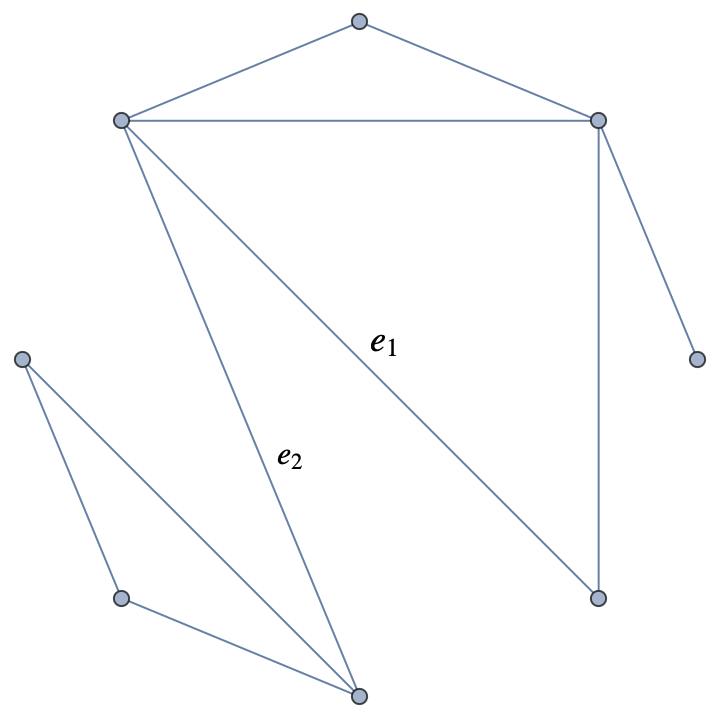
\includegraphics[width=\linewidth]{images/cup-graph.png}
\end{image}%
\tcblower
\end{figureptx}%
\begin{example}{Example}{Euler's Formula.}{example-s-induction-j}%
\index{Euler's Formula}%
Euler's Formula states that if \(G\) is a connected undirected planar graph, with \(v\) vertices, \(e\) edges and \(r\) regions, then \(v+r-e=2\)%
\par
We will prove this by induction on the number of edges in the graph.  Let \(p(n)\) be ``The statement is true for all such graphs with \(n\) edges, where \(n\geq 0\).''%
\par
Basis:  If a connected undirected planar graph has zero edges, it must be that the graph has only one vertex and the plane is  ``divided'' into only one region.  Therefore \(v=1\), \(e=0\), and \(r=1\); and   \(v+r-e=1+1-0 =2\).%
\par
Induction.  Assume Euler's formula is true for all connected undirected planar graphs  with \(k\) edges where \(k\leq n\).   Assume we such a graph, \(G\), with \(n+1\) edges.  We remove one of the edges from \(G\), making it an undirected planar graph with \(n\) edges.  However it may no longer be connected.  We need to consider two possible cases.%
\par
Case 1:  The graph with the removed edge is still connected. In the example above, if we remove \(e_1\), we have this situation.  Since we have a connected undirected planar graph with \(n\) edges, the induction hypothesis applied with \(k=n\), and so Euler's formula is true.  Now, consider returning the edge we had removed.  In so doing, the number of edges increases by 1, the number of verticies stays the same, and the number of regions increases by 1 since the returned edge divides a region into two parts.  Therefore, the net change in the expression \(v+r-e\) is \(0+1-1=0\)and so it is still equal to 2.%
\par
Case 2: The graph with the removed edge has two components. In the example above, if we remove \(e_2\), we have this situation.   The vertices in each of the two components are connected.  Assume the components have \(k_1\) and \(k_2\) edges, where \(k_1+k_2= n\).  Furthermore, assume the numbers of vertices and regions in the first component is \(v_1\) and \(r_1\), while the second component has \(v_2\) and \(r_2\) for it\textbraceleft{}'\textbraceright{}s vertices and regions. By the induction hyponthesis,%
\begin{equation*}
v_1+r_1-k_1=2 \textrm{ and } v_2+r_2-k_2=2
\end{equation*}
Now when we bring back the edge we had removed, the original graph had \(v_1+ v_2\) vertices and \(k_1+k_2+1= n+1\) edges.  The number of regions is \(r_1+ r_2-1\) because the infinite regions of the two components  is now one region.  Collecting this information, we have%
\begin{equation*}
\begin{split}
v+r-e &= \left(v_1+v_2\right)+\left(r_1+ r_2-1\right) -\left(k_1+k_2+1\right)\\
& = \left(v_1+r_1-k_1\right)+ \left(v_2+r_2+k_2\right) -2\\
&=2+2-2 = 2
\end{split}
\end{equation*}
Therefore Euler's formula is true for this case.%
\end{example}
\begin{example}{Example}{Recursive Thinking.}{example-determinant-sage-assist}%
Consider the sequence of  matrices \(A(n)\) defined by \(A(1)=[1]\) and for \(n \ge 1\), \(A(n)\) is an \((n-1) \times (n-1)\) identity matrix with a column of 1's appended to it, and then a row of 1's appended.  For example, \(A(3)=\begin{pmatrix}1 & 0 & 1\\
0 & 1 & 1\\
1 & 1 & 1 \end{pmatrix}\). What is the determinant of \(A(n)\)?%
\par
To solve this problem, we can expand the determinant along the first row.  This gives us two minors to evalute, one of which is the determinant of \(A(n-1)\).  The other minor is a matrix that takes a form like this one, in the case were we are expanding \(\lvert A(5)\rvert\): \(\begin{pmatrix}
0 & 1 & 0 & 0\\
0 & 0 & 1 & 0\\
0 & 0 & 0 & 1\\
1 & 1 & 1 & 1 \end{pmatrix}\).%
\par
By shifting the bottom row up, one row at a time, with \(n-2\) shifts, we get an upper triangular matrix with all 1's in the diagonal, and so the minor is  \((-1)^{(n-2)}\)  The cofactor corresponding to this minor will have a sign \((-1)^{n+1}\).  Therefore the value of the cofactor will be \((-1)^{n+1}\cdot (-1)^{(n-2)}= -1\) and so we have%
\begin{equation*}
\lvert A(n) \rvert = \lvert A(n-1) \rvert -1\text{.}
\end{equation*}
Since \(\lvert A(1) \rvert = 1\), we conclude that \(\lvert A(n) \rvert = 2-n \)%
\par
Occasionally, an assist from technology will jump-start a solution.  In this example, it might not be necessary. However, here is a verification that our solution was correct, or if you hadn't seen the recursion, it might serve as a hint.   Change the value of \mono{n} to see how the determinant depends on it.%
\begin{sageinput}
n=5
A=Matrix([[i==j or i==n-1 or j==n-1 for i in range(n)] for j in range(n)] )
[A,det(A)]
\end{sageinput}
\begin{sageoutput}
[[1 0 0 0 1]
[0 1 0 0 1]
[0 0 1 0 1]
[0 0 0 1 1]
[1 1 1 1 1], -3]
\end{sageoutput}
\end{example}
\end{sectionptx}
%
%
\typeout{************************************************}
\typeout{Section 2.2 The Pigeonhole Principle}
\typeout{************************************************}
%
\begin{sectionptx}{Section}{The Pigeonhole Principle}{}{The Pigeonhole Principle}{}{}{section-s-pigeons}
\index{Pigeonhole Principle}%
\begin{figureptx}{Figure}{More pigeons than pigeonholes.  Image by en:User:McKay CC-BY-SA-3.0 via Wikimedia Commons.}{figure-to-many-pigeons}{}%
\begin{image}{0}{1}{0}%
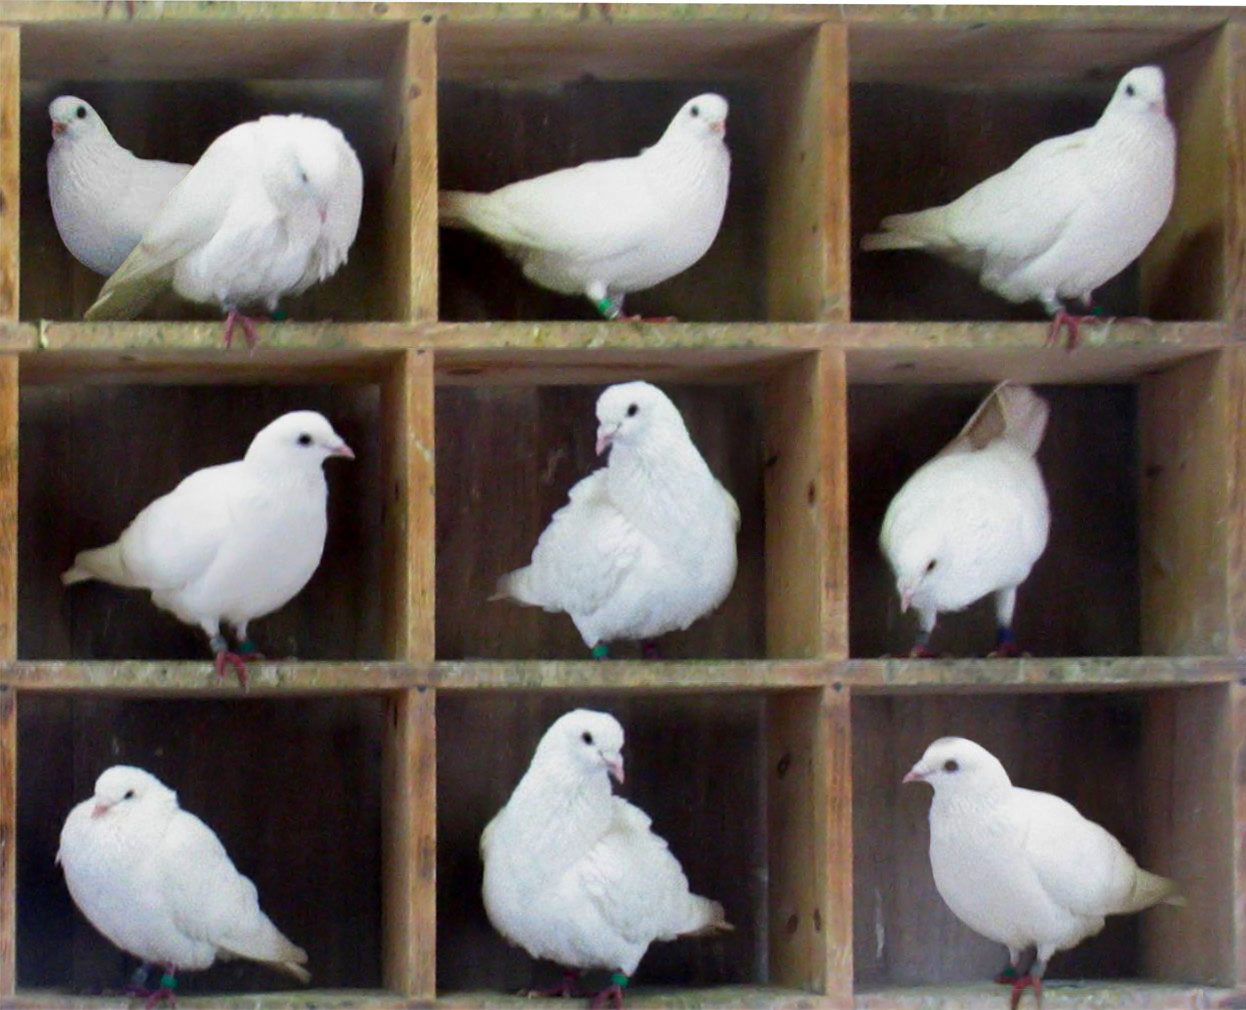
\includegraphics[width=\linewidth]{images/TooManyPigeons.jpg}
\end{image}%
\tcblower
\end{figureptx}%
Informally, the Pigeonhole Principle says that if you have more pigeons than you have pigeonholes, then at least one pair of pigeons have to share the same pigeonhole. The trick to using this simple idea is to identify the pigeons and pigeonholes in a problem.  Here is a relatively simple example. A clue that we can use the Pigeonhole Principle problem in this case is that we are asked to prove the existence of two objects that share a property.%
\begin{example}{Example}{}{example-e-pigeons-1}%
Prove that every set of 10 two-digit integer numbers has two disjoint subsets with the same sum of elements. (Subsets are pigeons, possible sums are holes)%
\par
We want two subsets with the same sum, so consider the possible sums to be pigeonholes, and now picture subsets of our ten integer set to be the pigeons. We are not given a specific set of integers, but we can identify the range of possible sums of elements in their subsets.  The smallest sum is 10 while the largest proper subset is \(91+92+\cdots+99 =855 \). That gives us 846 pigeonholes.  There are \(2^{10}-2 = 1022 > 845\) non-empty proper subsets of a ten element set.  Therefore, if we imagine each subset to roost with its sum, we are sure there there must be two subsets with the same sum.  Now those two subsets may not be disjoint, but if we simply remove elements in their intersection, we are done.%
\end{example}
\end{sectionptx}
%
%
\typeout{************************************************}
\typeout{Exercises 2.3 Problems}
\typeout{************************************************}
%
\begin{exercises-section}{Exercises}{Problems}{}{Problems}{}{}{exercises-induction-exercises}
\begin{divisionexercise}{1}{}{}{exercise-induction-exercises-b}%
Find and prove a formula for the sum of the first \(n\) consecutive odd positive integers. For example, if \(n = 4\) then \(1 + 3 + 5 + 7 = 16\).%
\par\smallskip%
\noindent\textbf{\blocktitlefont Hint}.\hypertarget{hint-induction-exercises-b-b}{}\quad{}Look at the first few examples.%
\par\smallskip%
\noindent\textbf{\blocktitlefont Solution}.\hypertarget{solution-induction-exercises-b-c}{}\quad{}First a bit of advice: It is often much easier to write a solution by ``inventing'' notation.  In this case, instead of referring to ``the sum of the first \(n\) consecutive odd positive integers,'' we define \(s(n)\) to be that sum.%
\par
We claim that \(s(n)=n^2\).  There are many proofs of this fact.  First we observe that the \(k\)th odd positive integer is \(2k-1\) and so \(s(n)=\sum_{k=1}^n 2k-1\)%
\par
The basis is clearly true:  \(s(1)=\sum_{k=1}^1 2k-1 = 1 = 1^2\).%
\par
Now assume that for some \(n\geq 1\) we have \(s(n)=n^2\).  Then%
\begin{equation*}
s(n+1) = \sum_{k=1}^{n+1} 2k-1= s(n) + 2n + 1 = n^2 + 2n +1 = (n+1)^2.
\end{equation*}
This completes the induction proof.%
\end{divisionexercise}%
\begin{divisionexercise}{2}{}{}{exercise-induction-exercises-c}%
Prove that in a room with \(n\) people, at least two people know exactly the same number of people. Assume knowing is a symmetric relation: If Paul knows Pat, then Pat knows Paul.%
\par\smallskip%
\noindent\textbf{\blocktitlefont Hint}.\hypertarget{hint-induction-exercises-c-b}{}\quad{}It is impossible to have someone know \(n-1\) people and someone else know nobody in the room.%
\end{divisionexercise}%
\begin{divisionexercise}{3}{}{}{exercise-induction-exercises-d}%
Let \(S\) be any set of 18 distinct integers chosen from the arithmetic progression \(1, 4, 7, \dots , 100\). Prove that there must be two integers in \(S\) whose sum is 101.%
\par\smallskip%
\noindent\textbf{\blocktitlefont Hint}.\hypertarget{hint-induction-exercises-d-b}{}\quad{}Count the number of pairs that can add up to 101.%
\par\smallskip%
\noindent\textbf{\blocktitlefont Solution}.\hypertarget{solution-induction-exercises-d-c}{}\quad{}Note that \(S\) is drawn from \(\{3i + 1 \vert 0 \leq i \leq 33 \}\), which contains 34 integers that can be paired up in such a way that if \(i + j = 33\), then  \((1+3i)+ (1+3j)=101\).  There are 17 such pairs, and so of the 18 elements in \(S\), at least one of the pairs that add to 101 must be included.%
\end{divisionexercise}%
\begin{divisionexercise}{4}{}{}{exercise-induction-exercises-e}%
Choose 51 positive integers from 1 to 100. Prove that one of them is a multiple of another.%
\par\smallskip%
\noindent\textbf{\blocktitlefont Hint}.\hypertarget{hint-induction-exercises-e-b}{}\quad{}Each integer has a maximal odd factor.%
\par\smallskip%
\noindent\textbf{\blocktitlefont Solution}.\hypertarget{solution-induction-exercises-e-c}{}\quad{}For each integer is in \(A = \{1, 2, 3, \dots, 100\}\) is equal to \(2^k m\), where \(m\) is an odd integer in \(B= \{1, 3, 5, \dots, 99\}\).  Since \(\lvert B \rvert =50\) and we have selected 51 integers from \(A\), there must be two in \(B\) with the form \(2^j n\) and \(2^k n\), where \(j \lt k\) and \(n \in B\), and we have the second as a multiple of the first.%
\end{divisionexercise}%
\begin{divisionexercise}{5}{}{}{exercise-induction-exercises-f}%
Show that a \(2^n \times  2^n\) square with a corner tile removed can be covered without overlaps by L-shaped figures (each figure contains 3 tiles). (If you feel adventurous, how about an \(n \times  n\) square for arbitrary \(n\)?)%
\end{divisionexercise}%
\begin{divisionexercise}{6}{}{}{exercise-induction-exercises-g}%
Given nine points inside the unit square, with no three colinear, prove that some three of them form a triangle whose area does not exceed \(1/8\).%
\end{divisionexercise}%
\begin{divisionexercise}{7}{}{}{exercise-induction-exercises-h}%
Prove that every positive integers is the sum of distinct nonconsecutive Fibonacci numbers.%
\par\smallskip%
\noindent\textbf{\blocktitlefont Solution}.\hypertarget{solution-induction-exercises-h-b}{}\quad{}We will prove this by induction. Starting with any positive integer, we remove the largest possible Fibonacci number to simplify the problem.  Our only concern is whether we would possibly need this Fibonacci number or the one before it to complete the desired sum.  For example, if we wish to write 2022 as a sum of Fibonacci numbers we can identify that \(1597\) is the largest such number less than or equal to 2022.  That leaves us with \(2022-1597=425\) to express as a sum of Fibonacci numbers.  We certainly can't use 1597 again, but the previous Fibonacci number, \(987\), is also too large to use in our sum.   Now let's look at a general proof.%
\par
Start by observing that 1 is a Fibonacci number.  Now assume that  all \(k\), \(1 \leq k \leq n\) are the sum of distinct nonconsecutive Fibonacci numbers.   Consider \(n+1\).  We are done if \(n+1\) is a Fibonacci number.   Otherwise, \(n+1\) is between Fibonacci numbers \(F_m\) and \(F_{m+1}\), and we use the former.%
\begin{equation*}
F_m \lt n+1 \lt F_{m+1} \quad	 \Rightarrow \quad  0\lt (n+1)-F_m \lt F_{m+1}-F_m = F_{m-1}
\end{equation*}
Since what is left if less than \(F_{m-1}\), we can apply the induction hypothesis to complete our decomposition of \(n+1\).%
\end{divisionexercise}%
\begin{divisionexercise}{8}{}{}{exercise-induction-exercises-i}%
Inside a circle of radius 4 are chosen 61 points. Show that among them there are two at distance at most \(\sqrt{2}\) from each other.%
\par\smallskip%
\noindent\textbf{\blocktitlefont Solution}.\hypertarget{solution-induction-exercises-i-b}{}\quad{}Solution 1:  If the center of the circle is placed at the origin of the Cartesian plane, we see that the interior can be divided into 60  one by one squares and partial squares.  Since there are 61 points, the Pigeonhole Principle can be applied, were any rule would be applied to point on the boundary of squares.%
\par
Solution 2:  For each point, place a disk of radius \(\frac{\sqrt{2}}{2}\) centered at that point. The area of each disk is \(\frac{\pi}{2}\).  The 61 disks cover a total area of \(\frac{61\pi}{2}\).  These disks are contained within a circle of area \((4+ \frac{\sqrt{2}}{2})^2 \pi\) which is less than \(\frac{61\pi}{2}\).  Therefore two of the disks must overlap and so their centers must be within \(\sqrt{2},\) of one another.%
\end{divisionexercise}%
\begin{divisionexercise}{9}{}{}{exercise-induction-exercises-j}%
Show that there is a positive term of the Fibonacci sequence that is divisible by 1000. Recall that the Fibonacci sequence is defined by \(F_0=0\), \(F_1= 1\) and for \(n>1\), \(F_n= F_{n-1}+F_{n-2}\). Note: The starting values of 0 and 1 are often replaced with 1 and 1, but for this problem it's slightly easier to structure a proof.%
\par\smallskip%
\noindent\textbf{\blocktitlefont Hint}.\hypertarget{hint-induction-exercises-j-b}{}\quad{}Start with two pairs of consecutive terms that have identical remainders mod 1000.%
\end{divisionexercise}%
\begin{divisionexercise}{10}{}{}{exercise-induction-exercises-k}%
You have coins \(C_1\), \(C_2\), ... , \(C_n\). For each \(k\), \(C_k\) is biased so that, when tossed, it has probability \(1/(2k + 1)\) of falling heads. If the \(n\) coins are tossed, what is the probability that the number of heads is odd? Express the answer as a rational function of \(n\).%
\par\smallskip%
\noindent\textbf{\blocktitlefont Answer}.\hypertarget{answer-induction-exercises-k-b}{}\quad{}The probability that the number of heads is odd is \(\frac{n}{2n+1}.\)%
\par\smallskip%
\noindent\textbf{\blocktitlefont Solution}.\hypertarget{solution-induction-exercises-k-c}{}\quad{}Let \(p_n\) be the probability that after tossing the first \(n\) coins, an odd number of heads have appeared.  Clearly \(p_1 = \frac{1}{3}\).  If \(n \gt 1\),%
\begin{equation*}
\begin{split}
p_n &= \frac{1}{2n+1}  (1-p_{n-1}) + \frac{2n}{2n+1} p_{n-1}\\
& = \frac{2n-1}{2n+1}p_{n-1} + \frac{1}{2n+1}
\end{split}
\end{equation*}
If you use the formula to compute a few more terms of the sequence, the pattern \(p_n=\frac{n}{2n+1} \) emerges and this can be proven by induction.%
\end{divisionexercise}%
\begin{divisionexercise}{11}{}{}{exercise-induction-exercises-l}%
Prove that any positive integer can be represented as \(\pm 1^2\pm 2^2\pm 3^2\pm \cdots \pm n^2\) for some positive integer \(n\) and some choice of signs.%
\end{divisionexercise}%
\begin{divisionexercise}{12}{}{}{exercise-induction-exercises-m}%
A fair coin is tossed repeatedly until there is a run of an odd number of heads followed by a tail. Determine the expected number of tosses.%
\par\smallskip%
\noindent\textbf{\blocktitlefont Hint}.\hypertarget{hint-induction-exercises-m-b}{}\quad{}Identify beginnings of the process that either end it or ``reset'' it.%
\par\smallskip%
\noindent\textbf{\blocktitlefont Solution}.\hypertarget{solution-induction-exercises-m-c}{}\quad{}If the first flip produces a tail, the expected length of the process from then on is the same as the expectation before that flip.   The same is true if the first two flips come up heads.  If the first two flips are heads-tails, the process has ended in two flips.  One of these three possible beginnings will occur with probabilities \(1/2\), \(1/4\), and \(1/4\), respectively.  Therefore if \(F\) is the expected number of flips, we have%
\begin{equation*}
\frac{1}{2} (1+F) +\frac{1}{4} (2+F) +\frac{1}{4} (2) = F\text{.}
\end{equation*}
Solving for \(F\), we get 6 for the expected number of flips.%
\end{divisionexercise}%
\begin{divisionexercise}{13}{}{}{exercise-induction-exercises-n}%
Show that every set of \(n\) integers has a nonempty subset such that the sum of its elements is divisible by \(n\).%
\par\smallskip%
\noindent\textbf{\blocktitlefont Solution}.\hypertarget{solution-induction-exercises-n-b}{}\quad{}Let \(a_1, a_2, \dots , a_n\) be the integers and let \(s_1, s_2, \dots , s_n\) be the partial sums, \(s_k=\sum _{i=1}^k
a_i\).  If one of the sums is divisible by \(n\) then we are done, so assume none are multiples of \(n\).  By the pigeonhole principle, there must be two partial sums that have the same residue mod \(n\).  Let \(l \lt m \) be such that%
\begin{equation*}
s_l\equiv s_m \pmod{n} \Rightarrow s_m-s_l= \sum _{k=l+1}^m a_k=n q
\end{equation*}
for some integer \(q\).  Therefore the set we are looking for is \(\left\{a_{l+1}, \ldots, a_m\right\}\).%
\end{divisionexercise}%
\begin{divisionexercise}{14}{}{}{exercise-induction-exercises-o}%
Show that for any polynomial \(f(x)\) over the integers with degree \(d\lt n\), we have \(\sum_{k=0}^{n} (-1)^k \binom{n}{k} f(k) = 0\).%
\par\smallskip%
\noindent\textbf{\blocktitlefont Solution}.\hypertarget{solution-induction-exercises-o-b}{}\quad{}(Solution by Tung Nguyen) Proof by induction on \(d\). Denote \(f(x) = \sum_{i = 0}^{d} a_i x^i\), where \(a_i\) are integer coefficients.  If \(d=0\), then functions \(f(x)\) of degree 0 are constant, i.e. \(f(x) = c\) for some \(c \in \mathbb{Z}\). This leads to%
\begin{equation}
\begin{split}
\sum_{k=0}^{n} (-1)^k\binom{n}{k}f(k) & = \sum_{k=0}^{n} (-1)^k\binom{n}{k}c\\
& = c\sum_{k=0}^{n} (-1)^k\binom{n}{k}(1)^{n-k} \\
& = c(1 - 1)^n = 0
\end{split}\label{men-sum0}
\end{equation}
for all positive integers \(n \gt 0 = d\). Note at if \(n = 0\) the sum above is \(c\) instead of \(0\).%
\par
Assume that the formula is true for every polynomial of degree \(d\) and applicable to all \(n \in \mathbb{N}\) satisfying \(d \lt n - 1\). We will prove that the formula is true for \(d + 1 \lt n\).%
\par
Let \(g(x)\) be an arbitrary polynomial of degree \(d+1\) over the integers, then \(g(x)\) can be rewritten as \(g(x) = x\cdot h(x) + c\), where \(h(x)\) has degree \(d\) and \(c\) is an integer. Then%
\begin{equation}
\begin{split}
\sum_{k=0}^{n} (-1)^k\binom{n}{k}g(k) &= \sum_{k=0}^{n} (-1)^k\binom{n}{k}\left[kh(k) + c\right]\\
& = \sum_{k=0}^{n} (-1)^k\binom{n}{k}k \cot h(k) + \sum_{k=0}^{n} (-1)^k\binom{n}{k}c.
\end{split}\label{men-sum1}
\end{equation}
The second term is 0 which is proven by \hyperref[men-sum0]{({\xreffont\ref{men-sum0}})}, while%
\begin{equation}
\begin{split}
\sum_{k=0}^{n} (-1)^k\binom{n}{k}k\cdot h(k) 
&= (-1)^0\binom{n}{0}0\cdot h(0) + \sum_{k=1}^{n} (-1)^k\frac{n!}{k!(n-k)!}k\cdot h(k)\\
& = 0 + \sum_{k=1}^{n} (-1)^k\frac{n!}{(k-1)!(n-k)!}h(k)\\
& = -n\sum_{k=1}^{n} (-1)^{k-1}\frac{(n-1)!}{(k-1)!(n-k)!}h(k) \\ 
&= -n\sum_{k=1}^{n} (-1)^{k-1}\binom{n-1}{k-1}h(k)\\
& = -n\sum_{k=0}^{n-1} (-1)^k\binom{n-1}{k}h(k+1)
\end{split}\label{men-sum2}
\end{equation}
%
\par
Because \(h(x)\) has degree \(d\), \(h(x+1)\) is also has degree \(d\), which is less than \(n - 1\) by the induction hypothesis. Therefore we have%
\begin{equation}
\sum_{k=0}^{n-1} (-1)^k\binom{n-1}{k}h(k+1)  = 0 \label{men-sum3}
\end{equation}
%
\par
Combining \hyperref[men-sum1]{({\xreffont\ref{men-sum1}})},\hyperref[men-sum2]{({\xreffont\ref{men-sum2}})} and \hyperref[men-sum3]{({\xreffont\ref{men-sum3}})} together, we have \(\sum_{k=0}^{n} (-1)^k\binom{n}{k}g(k) = 0\). Because \(g(x)\) is arbitrarily chosen, the formula must be true for all polynomials of degree \(d + 1 \lt n\), completing the induction.%
\end{divisionexercise}%
\begin{divisionexercise}{15}{}{}{exercise-induction-exercises-p}%
Given a sequence of integers \(x_1\), \(x_2\), \(\dots x_n\) whose sum is 1, prove that exactly one of the cyclic shifts%
\begin{gather*}
x_1,x_2,\dots ,x_n \\
x_2,\dots,x_n,x_1  \\
\vdots    \\
x_n,x_1,\dots,x_{n-1}  
\end{gather*}
has all of its partial sums positive. (By a partial sum we mean the sum of the first \(k\) terms, \(k \leq  n\).%
\par\smallskip%
\noindent\textbf{\blocktitlefont Solution}.\hypertarget{solution-induction-exercises-p-b}{}\quad{}We define a ``good shift'' to be one for which the partial sums are all positive. The property we wish to prove is obviously true for \(n=1\).  Now assume that for some \(n \geq 1\) that it's true for all sequences of length \(n\).  Consider an integer sequence of length \(n+1\).  Since the sum of the terms is 1, there must exist at least one negative term and among them all, there must be one that is preceded by a positive term. We can assume that these two terms are at the end of the sequence, \(x_n, x_{n+1}\).  Now consider the sequence of length \(n\) defined by \(y_j = x_j\) if \(j \lt n\)  and  \(y_n=x_n+x_{n+1}\).  By the induction hypothesis, this sequence has a unique good shift.  In that shifted sequence, wherever \(y_n\) is located  we replace it with the two terms \(x_n, x_{n+1}\). The partial sums of this expanded sequence are still all positive so we have a good shift of the original sequence.  Finally, we see that this good shift is unique. Every good shift of the original sequence can produce a good shift of the reduced \(y\)-sequence and we know that only one of those exists.%
\end{divisionexercise}%
\end{exercises-section}
\end{chapterptx}
%
%
\typeout{************************************************}
\typeout{Chapter 3 Tricks of the Trade}
\typeout{************************************************}
%
\begin{chapterptx}{Chapter}{Tricks of the Trade}{}{Tricks of the Trade}{}{}{chapter-c-tricks}
\renewcommand*{\chaptername}{Chapter}
\begin{introduction}{}%
In this chapter we highlight some ``tricks of the trade'' that can help you piece together a solution to many problems.  Naturally, no single trick is likely to be needed in a given competition, but all of them have been played a part in solving some problems in past competitions.%
\end{introduction}%
%
%
\typeout{************************************************}
\typeout{Section 3.1 Telescoping Sums}
\typeout{************************************************}
%
\begin{sectionptx}{Section}{Telescoping Sums}{}{Telescoping Sums}{}{}{section-c-tricks-c}
\index{Telescoping Sum}%
Telescoping sums are occasionally embedded in more challenging problems than this one.%
\begin{example}{Example}{}{example-c-tricks-c-d}%
Let \(f(n)=\sum_{k=1}^n \frac{1}{\sqrt{k}+\sqrt{k+1}}\).  Evaluate \(f(9999)\).%
\par
Rationalizing the denominator reveals a \terminology{telescoping sum} here.  For any nonnegative \(k\),%
\begin{equation*}
\begin{split}
\frac{1}{\sqrt{k} + \sqrt{k + 1}} & = \frac{\sqrt{k + 1} - \sqrt{k}}{(\sqrt{k} + \sqrt{k + 1})(\sqrt{k + 1} - \sqrt{k})}\\ 
&= \frac{\sqrt{k + 1} - \sqrt{k}}{k + 1 - k}\\
&= \sqrt{k + 1} - \sqrt{k}
\end{split}\text{.}
\end{equation*}
So \(f(9999) = \sum_{1}^{9999}(\sqrt{k + 1} - \sqrt{k}) = \sqrt{9999 + 1} - \sqrt{1} = 100 - 1 = 99\).  (Solution by Tung Nguyen)%
\end{example}
\end{sectionptx}
%
%
\typeout{************************************************}
\typeout{Section 3.2 Completing the Product}
\typeout{************************************************}
%
\begin{sectionptx}{Section}{Completing the Product}{}{Completing the Product}{}{}{section-c-tricks-d}
The elementary trick of completing the square, given a quadratic and linear term, can be generalized.  Given three terms, completing the product of two binomials can play a part in a solution.  This occured in the 2018 Putnam, problem A1.%
\begin{quote}%
Find all ordered pairs \((a,b)\) of positive integers for which%
\begin{equation*}
\frac{1}{a} + \frac{1}{b} = \frac{3}{2018}.
\end{equation*}
%
\end{quote}
Elementary algebra leads to%
\begin{equation*}
3ab-2018(a+b)=0
\end{equation*}
By distributing the 2018 we have three terms.  Multiplying by 3 and adding \(2018^2\) to both sides completes a product of two binomial factors on the the left side:%
\begin{equation*}
(3a-2018)(3b-2018) = 2018^2.
\end{equation*}
%
\begin{aside}{Aside}{On year numbers..}{aside-c-tricks-d-e}%
Problem posers often like to involve the current year in at least one problem in a competition; so it's a good idea to be familiar with the current year's factorization.%
\end{aside}
From the Putnam Archive:%
\begin{quote}%
With this equation, we can identify solutions the original equation in the positive integers. Each of the factors is congruent to \(1 \pmod 3\). There are \(6\) positive factors of \(2018^2 = 2^2 \cdot 1009^2\) that are congruent to \(1 \pmod 3\): \(1\), \(2^2\), \(1009\), \(2^2 \cdot 1009\), \(1009^2\), \(2^2 \cdot 1009^2\). These lead to the \(6\) possible pairs: \((a,b) = (673,1358114)\), \((674,340033)\), \((1009,2018)\), \((2018,1009)\), \((340033,674)\), and \((1358114,673)\).%
\par
As for negative factors, the ones that are congruent to \(1 \pmod 3\) are \(-2, -2 \cdot 1009, -2 \cdot 1009^2\).  However, all of these lead to pairs where \(a \leq 0\) or \(b \leq 0\).%
\end{quote}
\end{sectionptx}
%
%
\typeout{************************************************}
\typeout{Section 3.3 Trig Substitution}
\typeout{************************************************}
%
\begin{sectionptx}{Section}{Trig Substitution}{}{Trig Substitution}{}{}{section-c-tricks-e}
When real numbers are known to have absolute value less than or equal to 1, consider equating them with cosines or sines.   Here is an example from the 2000 Putnam, Problem B4.%
\begin{example}{Example}{2000 Putnam, B4.}{example-ex-2000PutnamB4}%
Let \(f:[-1,1]\rightarrow \mathbb{R}\) be a continuous function such that \(f(2x^21)=2xf(x)\) for all \(x\). Show that \(f(x)=0\) for \(-1 \leq x \leq 1\).%
\par
Solution: Substitution of 1 and -1 for \(x\) produces \(f(1)=f(-1)=0\).%
\par
The restriction on \(x\) and the expression \(2 x^2 -1\) may remind one of the identity \(2\cos^2{x} - 1 = \cos{2 x}\); and so the substitution \(x = \cos{t}\) is a reasonable step leading to \(f(\cos{2t})=2 \cos{t} f(\cos{t})\).%
\par
The next step in several published solutions is to define a second function, \(g\), by%
\begin{equation*}
g(t)=\frac{f(\cos{t})}{\sin{t}}, \textrm{ where } t\neq \pi k, k\in \mathbb{Z}
\end{equation*}
%
\begin{aside}{Aside}{}{aside-ex-2000PutnamB4-f}%
A ``meta exercise'' is to provide a motivation for this definition of \(g\).%
\end{aside}
%
\begin{equation*}
g(2t)=\frac{f(\cos{2t})}{\sin{2t}}=\frac{2 \cos{t}\: f(\cos{t})}{2\sin{t}\cos{t}}=g(t)
\end{equation*}
Combining this with the periodicity of \(g\) tells us that%
\begin{equation*}
g(1+\frac{n \pi}{2^k})=g(2^{k+1}+2 \pi n) = g(2^{k+1})=g(1)
\end{equation*}
The continuity of \(g\) in its domain and the density of \(\{1+\frac{n \pi}{2^k} \mid n,k \in \mathbb{Z}\}\) implies that \(g\) must be constant.%
\par
Returning our attention to \(f\) we have \(f(\cos{t})= c \sin{t}\) for some constant \(c\), which implies \(f(x) = c \sqrt{1-x^2}\) for \(x \in (-1,1)\).  Finally, this tells us that \(f\) must be even.  However, when we turn to the original fuctional equation, \(x f(x)=f(2x^2-1)\) we have an odd function on the left and an even function on the right.  Our only possibility is the desired conclusion.%
\end{example}
\end{sectionptx}
%
%
\typeout{************************************************}
\typeout{Section 3.4 Generalization}
\typeout{************************************************}
%
\begin{sectionptx}{Section}{Generalization}{}{Generalization}{}{}{section-c-tricks-f}
Many mainstream topics in the mathematics curriculum can be generalized. One example is the binomial expansion.  The expansion of \((x+y)^n\) for nonnegative integers is in every curriculum, but its generalization for non-integral exponents is not.%
\begin{example}{Example}{Fractional Binomial Expansion.}{example-c-tricks-f-c}%
\index{Fractional Binomial Expansion}%
The power series series expansion about \(x=0\) of an expression such as \(\sqrt{1-x}\) certainly can be derived using basic calculus tools, but an alternate approach can be taken by (correctly) assuming that the binomial expansion theorem applies for the exponent \(\frac{1}{2}\).  If \(m\) is a positive integer, \(\binom{m}{n} =0\) for \(n \gt m\), but a reasonable generalization of \(\binom{\alpha}{n}\) for a non-integer \(\alpha\) is%
\begin{equation*}
\frac{\prod_{k=0}^{n-1} (\alpha-k)}{n!}
\end{equation*}
which will never equal zero for non-integral values of \(\alpha\).  Thus we have%
\begin{equation*}
\sqrt{1-x} = \sum_{n=0}^{\infty} \binom{\frac{1}{2}}{n} (-x)^n
\end{equation*}
The first two terms of this sum are 1 and \(-\frac{1}{2} x\). We will proceed to simplify the general form of the coefficient of \(x^n\) for \(n \gt 1\).%
\begin{equation*}
\begin{split}
\binom{\frac{1}{2}}{n} (-1)^n
&=  \frac{\frac{1}{2} \cdot\frac{-1}{2}\cdot\frac{-3}{2}\cdot \cdots \cdot(\frac{1}{2}-(n-1)) }{n!} (-1)^n\\
\textrm{multiply fractions by 2 }	&=  \frac{1 \cdot -1 \cdot -3 \cdot \cdots \cdot (-2n+3)}{2^{n} n!} (-1)^n\\
\textrm{multiply negatives by factors of -1}	&= - \frac{1 \cdot 1 \cdot 3 \cdot \cdots \cdot (2n-3)}{2^{n} n!}  \\
\textrm{fill in even and higher factors of }(2n!)	&= - \frac{ 1 \cdot 2 \cdot 3\cdot 4 \cdot \cdots \cdot (2n-3)\cdot (2n-2)\cdot (2n-1)\cdot (2n)}{2^n\cdot 2^n\cdot (n!)^2 \cdot (2n-1)}  \\
\textrm{(put things together)}	&= - \frac{(2n)!}{4^n \cdot(n!)^2\cdot (2n-1)} 
\end{split}
\end{equation*}
This general formula actually works for all \(n\), including 0 and 1.   Thus,%
\begin{equation*}
\sqrt{1-x}  = - \sum_{n=0}^{\infty} \frac{(2n)!}{4^n \cdot(n!)^2\cdot (2n-1)}  x^n  
\end{equation*}
%
\end{example}
\begin{remark}{Remark}{}{remark-c-tricks-f-d}%
\index{Pochhammer symbol} The Pochhammer symbol is the notation  \((x)_n\), where \(n\) is a non-negative integer. It is commonly used to represent the ``falling factorial'' expression  \(x\cdot(x-1)\cdot(x-2)\cdot \cdots \cdot (x-(n-1))\).  This gives a more concise way to express the expansion we have just examined as \(\sum_{n=0}^{\infty} \frac{(\frac{1}{2})_n}{n!} (-x)^n\).  However, you still need to get into the weeds and manipulate the expression in the end.%
\end{remark}
A different sense in which generalization applies to problem solving is when a problem is more easily solved by first generalizing the context of the problem.  This problem from the 1982 Putnam is a good example.%
\begin{example}{Example}{A Putnam Integral.}{example-example-putnam-integral}%
\index{Leibniz Integration Rule}%
Evaluate \(\int_0^{\infty} \frac{\tan^{-1}(\pi  x)-\tan^{-1}(x)}{x} \, dx\).%
\par
The integral can be evaluated by generalizing it first to a function: \(F(y)=\int_0^{\infty} \frac{\tan ^{-1}(y x)-\tan ^{-1}(x)}{x} \, dx\). We then can differentiate with respect to \(y\) to get a simple expression of \(F(y)\).  After applying the obvious condition \(F(1)=0\), we can substitute \(\pi\) for \(y\) to get our final answer.  We leave it as an exercise for you to get the final answer of \(\frac{1}{2} \pi  \ln(\pi )\).   The fact that we can of differentiant inside an integral as is suggested here is referred to as the \terminology{Leibniz Integration Rule}.%
\end{example}
\end{sectionptx}
%
%
\typeout{************************************************}
\typeout{Exercises 3.5 Exercises}
\typeout{************************************************}
%
\begin{exercises-section}{Exercises}{Exercises}{}{Exercises}{}{}{exercises-c-tricks-g}
\begin{divisionexercise}{1}{}{}{exercise-c-tricks-g-b}%
Let \(a, b, c \in [0, 1]\). Prove that%
\begin{equation*}
\sqrt{a b c}+ \sqrt{(1-a)(1-b)(1-c)} \leq 1
\end{equation*}
%
\par\smallskip%
\noindent\textbf{\blocktitlefont Hint}.\hypertarget{hint-c-tricks-g-b-b}{}\quad{}Start with proving  \(\sqrt{a b}+ \sqrt{(1-a)(1-b)} \leq 1\)%
\end{divisionexercise}%
\begin{divisionexercise}{2}{}{}{exercise-c-tricks-g-c}%
Evalute \(\int x^3 \sqrt{4-9x^2} \, dx\)%
\par\smallskip%
\noindent\textbf{\blocktitlefont Solution}.\hypertarget{solution-c-tricks-g-c-b}{}\quad{}Use the substitution \(x = \frac{2}{3} \sin{\theta}\).  The final value is \(-\frac{\left(4-9 x^2\right)^{3/2}
\left(27 x^2+8\right)}{1215}\).%
\end{divisionexercise}%
\begin{divisionexercise}{3}{}{}{exercise-c-tricks-g-d}%
For any triangle \(ABC\), prove that%
\begin{equation*}
\tan{A}+\tan{B}+\tan{C} = \tan{A}\cdot \tan{B}\cdot \tan{C}
\end{equation*}
%
\end{divisionexercise}%
\begin{divisionexercise}{4}{}{}{exercise-c-tricks-g-e}%
Let \(f(x)=\frac{1}{\sqrt{1+x}}\).  Estimate the value of \(f(\frac{1}{2})\) with a fractional binomial expansion so that the error is less than \(\frac{1}{100}\).%
\par\smallskip%
\noindent\textbf{\blocktitlefont Solution}.\hypertarget{solution-c-tricks-g-e-b}{}\quad{}The fractional binomial expansion of \(f(x)\) is the alternating series%
\begin{equation*}
1 - \frac{1}{2} x +  \frac{3}{8} x^2- \frac{5}{16} x^3 +  \frac{35}{128} x^4 - \cdots 
\end{equation*}
which converges when \(x=\frac{1}{2}\).   The fourth degree term at \(\frac{1}{2}\) has a value less than \(\frac{1}{100}\), and so we can estimate the value of \(f(\frac{1}{2})\) with sufficient accuracy by adding the previous terms, which gives us an estimate of \(\frac{103}{128}\).%
\end{divisionexercise}%
\begin{divisionexercise}{5}{}{}{exercise-c-tricks-g-f}%
Complete the derivation of the value of the integral in \hyperref[example-example-putnam-integral]{Example~{\xreffont\ref{example-example-putnam-integral}}}.%
\end{divisionexercise}%
\begin{divisionexercise}{6}{}{}{exercise-c-tricks-g-g}%
Evaluate \(\int_0^1 \frac{t^3-1}{\log (t)} \, dt\).%
\par\smallskip%
\noindent\textbf{\blocktitlefont Solution}.\hypertarget{solution-c-tricks-g-g-b}{}\quad{}Let \(G(x)=\int_0^1 \frac{t^x-1}{\log (t)} \, dt \). By the Leibniz Integration Rule,%
\begin{equation*}
G'(x)=\int_0^1 \partial_x \left(\frac{t^x-1}{\ln(t)}\right)\, dt = \int_0^1 t^x \, dt = \frac{1}{x+1}.
\end{equation*}
Therefore,  \(G(x) = \ln{\lvert x+1 \rvert} + C\), and since \(G(0)=0\), \(C=0\).   Finally we get \(G(3) = ln(4)\).%
\end{divisionexercise}%
\end{exercises-section}
\end{chapterptx}
%
%
\typeout{************************************************}
\typeout{Chapter 4 Counting and Indirect Proofs}
\typeout{************************************************}
%
\begin{chapterptx}{Chapter}{Counting and Indirect Proofs}{}{Counting and Indirect Proofs}{}{}{chapter-c-counting}
\renewcommand*{\chaptername}{Chapter}
%
%
\typeout{************************************************}
\typeout{Section 4.1 Counting Two Ways}
\typeout{************************************************}
%
\begin{sectionptx}{Section}{Counting Two Ways}{}{Counting Two Ways}{}{}{section-c-counting-b}
Most students are familiar with formula for a binomial coefficient,\(\binom{n}{k}\). Here, we will derive the formula by two-way counting.%
\begin{example}{Example}{}{example-ex-binomial-coeff-formula}%
The binomial coefficient \(\binom{n}{k}\) represents the  the number of \(k\) element subsets of an \(n\) element set , \(0\leq k\leq n\).%
\par
We will count the number of ways to permute \(k\)  objects from a set of \(n\) elements two ways.  First, we can first choose one of the \(k\) element subsets of of the set, and second, choose one of the \(k!\)  permutations of those elements. By the rule of products, we can do this \(\binom{n}{k} \cdot k!\).  A second approach is to select the the elements from our set to go into positions 1 through \(k\) in the permutation immediately.  The number of ways of doing this is \(n \cdot (n-1)\cdot \cdots \cdot (n-(k-1))\).   The two expressions count the same number and so they are equal. We equate them and then solve for the value of the  binomial coefficient:  \(\binom{n}{k} =\frac{n!}{k! \cdot (n-k)!}\).%
\end{example}
\end{sectionptx}
%
%
\typeout{************************************************}
\typeout{Section 4.2 Indirect Proofs}
\typeout{************************************************}
%
\begin{sectionptx}{Section}{Indirect Proofs}{}{Indirect Proofs}{}{}{section-c-counting-c}
\begin{example}{Example}{No Least Positive Real Number.}{example-c-counting-c-b}%
Prove that there is no least positive real number.%
\par
Assume that there is a least positive real number, which we'll call \(L\).  Certainly, we can assume that \(L \lt 1\) since we know of many positive real number that statisfy this inequality.  If we multiply the inequality by \(L\), we find that \(L^2 \lt L\).  Since \(L^2\) is a positive real number we have a contradiction that \(L\) is least.  Hence no such least number can exist.%
\end{example}
\begin{example}{Example}{The Harmonic Series.}{example-c-counting-c-c}%
\index{Harmonic Series}%
Students often struggle with the idea that although the terms of the harmonic series, \(\sum_{n=1}^{\infty} \frac{1}{n}\), converge to zero, the series itself diverges. Encountering this fact in a calculus class in which proof may not be emphasized is often the problem.  Many of the dozens of proofs that the harmonic series diverges are indirect.  Here is one such example.%
\par
Assume the series converges and its limit is \(H\).%
\begin{equation*}
\begin{split}
H &= 1 + \frac{1}{2} + \frac{1}{3} + \frac{1}{4} +\cdots + \frac{1}{2k-1} + \frac{1}{2k} + \cdots\\
& \gt  \frac{1}{2} + \frac{1}{2} + \frac{1}{4} + \frac{1}{4} +\cdots + \frac{1}{2k} + \frac{1}{2k} + \cdots\\
& = 1 + \frac{1}{2} +  +\cdots + \frac{1}{k}  + \cdots\\
& = H
\end{split}
\end{equation*}
The contradiction we arrive at, \(H \gt H\), implies that the series does indeed diverge.%
\end{example}
\end{sectionptx}
%
%
\typeout{************************************************}
\typeout{Exercises 4.3 Problems}
\typeout{************************************************}
%
\begin{exercises-section}{Exercises}{Problems}{}{Problems}{}{}{exercises-c-counting-d}
\begin{divisionexercise}{1}{}{}{exercise-c-counting-d-b}%
Let \(S\) be a set of real numbers which is closed under multiplication (that is, if \(a\) and \(b\) are in \(S\), then so is \(a b\)). Let \(T\) and \(U\) be disjoint subsets of \(S\) whose union is \(S\). Given that the product of any three (not necessarily distinct) elements of \(T\) is in \(T\) and that the product of any three elements of \(U\) is in \(U\), show that at least one of the two subsets \(T\), \(U\) is closed under multiplication.%
\par\smallskip%
\noindent\textbf{\blocktitlefont Solution}.\hypertarget{solution-c-counting-d-b-b}{}\quad{}Assume neither \(T\) nor \(U\) is closed.  Then there exist \(t_1, t_2\in T\) and \(u_1, u_2 \in U\) such that \(t_1\cdot t_2 \in U\) and \(u_1 \cdot u_2 \in T\).  We can observe that \((t_1\cdot t_2)\cdot(u_1 \cdot u_2)\) is a product of either three elements of \(T\), or a product of three elements of \(U\), meaning that it would be in the intersection, which is a contradiction.  Therefore one of the sets is closed.%
\end{divisionexercise}%
\begin{divisionexercise}{2}{}{}{exercise-c-counting-d-c}%
Let's say I have a group of \(n+1\) people who want to see a show. Assume they all have different ages.  I have three tickets into the theatre: a backstage pass and two regular (but distinguishable) tickets. I have to give out the tickets according to the following two rules:%
\begin{enumerate}[label=(\alph*)]
\item{}The backstage pass must go to the oldest person who gets a ticket.%
\item{}The person who gets the backstage pass can't get either of the other two tickets. The two regular tickets can go to the same person or to two different people.%
\end{enumerate}
How many ways can I give away the tickets? There are two ways to count. Find both and equate them.%
\par\smallskip%
\noindent\textbf{\blocktitlefont Hint}.\hypertarget{hint-c-counting-d-c-b}{}\quad{}You get two different results depending on whether you select who will be oldest first, or you decide what three people will get tickets first.%
\end{divisionexercise}%
\begin{divisionexercise}{3}{Lattice Paths.}{}{exercise-c-counting-d-d}%
\index{Lattice Paths}%
Consider paths such as the one in the grid below that start at the bottom left, \((0,0),\) and reach the top right, \((10,10)\).  These paths can only go up and to the right.  How many paths are there in all? How many of those paths pass through the point \((4,6)\)?  Generalize both of your results.%
\begin{figureptx}{Figure}{A Lattice Path}{figure-lattice_path}{}%
\begin{image}{0.2}{0.6}{0.2}%
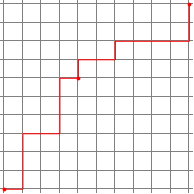
\includegraphics[width=\linewidth]{images/lattice_path.png}
\end{image}%
\tcblower
\end{figureptx}%
\par\smallskip%
\noindent\textbf{\blocktitlefont Hint}.\hypertarget{hint-c-counting-d-d-d}{}\quad{}Think of each path as a sequence of instructions to go right (R) and up (U).%
\par\smallskip%
\noindent\textbf{\blocktitlefont Answer}.\hypertarget{answer-c-counting-d-d-e}{}\quad{}There are \(\binom{m+n}{m}\) paths%
\par\smallskip%
\noindent\textbf{\blocktitlefont Solution}.\hypertarget{solution-c-counting-d-d-f}{}\quad{}Each path can be described as a sequence or R's and U's with exactly ten of each.   The ten positions in which R's could be placed can be selected from the twenty positions in the sequence \(\binom{20}{10}\) ways.  We can generalize this logic and see that there are \(\binom{m+n}{m}\) paths from \((0,0)\) to \((m,n)\).%
\end{divisionexercise}%
\begin{divisionexercise}{4}{}{}{exercise-c-counting-d-e}%
Prove that if \(n\geq 1\), then \(\sum _{k=0}^n \binom{n}{k}^2=\binom{2 n}{n}\)%
\par\smallskip%
\noindent\textbf{\blocktitlefont Hint}.\hypertarget{hint-c-counting-d-e-b}{}\quad{}Consider the lattice paths from \((0,0)\) to \((n,n)\) passing through any point on the diagonal \(i + j = n\).%
\end{divisionexercise}%
\begin{divisionexercise}{5}{}{}{exercise-c-counting-d-f}%
Prove that the number of odd coefficients in each row of Pascal's triangle is a power of 2.%
\par\smallskip%
\noindent\textbf{\blocktitlefont Solution}.\hypertarget{solution-c-counting-d-f-b}{}\quad{}%
\end{divisionexercise}%
\begin{divisionexercise}{6}{}{}{exercise-c-counting-d-g}%
Every point of three-dimensional space is colored red, green, or blue. Prove that one of the colors attains all distances, meaning that any positive real number represents the distance between two points of this color.%
\par\smallskip%
\noindent\textbf{\blocktitlefont Hint}.\hypertarget{hint-c-counting-d-g-b}{}\quad{}If false, there are ``non-attainable'' distances for each color. Select one for each color.%
\par\smallskip%
\noindent\textbf{\blocktitlefont Solution}.\hypertarget{solution-c-counting-d-g-c}{}\quad{}If false, there are ``non-attainable'' distances for each color. Select one for each color.  Call them \(r\), \(g\) and \(b\), with  \(r \geq g \geq b\).  Select any red point, call it \(R\), and consider the surface of the sphere of radius \(r\) centered at \(R\).   This is a blue\slash{}green sphere.   Now select any green point, \(G\) on the surface. If we consider \(G\) to be a pole of the blue\slash{}green sphere, the intersection of the blue\slash{}green sphere with the sphere of radius \(g\)  centered at \(G\) is a parallel on the blue\slash{}green sphere that is blue.  Given our assumptions about the unattainable distances, there must be points on the blue parallel that are \(b\) units apart, which is a contradiction.%
\end{divisionexercise}%
\begin{divisionexercise}{7}{}{}{exercise-c-counting-d-h}%
The union of nine planar surfaces, each of area equal to 1, has a total area equal to 5. Prove that the overlap of some two of these surfaces has an area greater than or equal to \(\frac{1}{9}\).%
\par\smallskip%
\noindent\textbf{\blocktitlefont Solution}.\hypertarget{solution-c-counting-d-h-b}{}\quad{}Let us assume that the area of the overlap of any two surfaces is less than \(\frac{1}{9}\). In this case, if \(S_1, S_2, \dots , S_9\)  denote the nine surfaces, then the area of \(S_1 \cup S_2\) is greater than \(1 + 8/9\) , the area of \(S_1 \cup S_2 \cup S_3\) is greater than \(1 + 8/9 + 7/9\), and we continue this line of reasoning to conclude that the area of the union of all nine regions must be greater than%
\begin{equation*}
1 + 8/9 + 7/9 + \dots + 1/9 = 45/9 = 5
\end{equation*}
which is a contradiction. Hence the conclusion%
\end{divisionexercise}%
\begin{divisionexercise}{8}{}{}{exercise-c-counting-d-i}%
Prove that there is no polynomial with integer coefficients \(P(x)\) with the property that \(P(7) = 5\) and \(P(15) = 9\).%
\par\smallskip%
\noindent\textbf{\blocktitlefont Solution}.\hypertarget{solution-c-counting-d-i-b}{}\quad{}Let \(Q(x)=P(x)-5\).  On one hand, \(Q(15)=P(15)-5 = 4\).  However, since \(Q(7)=0\), \(Q(x)=(x-7)R(x)\) for some polynomial \(R(x)\) which has integer coefficients.  But \(Q(15)=(15-7)R(15)=8 R(15)\) is a multiple of \(8\).  Which contradicts our previous value of \(4\).%
\end{divisionexercise}%
\begin{divisionexercise}{9}{}{}{exercise-c-counting-d-j}%
How many positive integers not exceeding 2019 are multiples of 3 or 4 but not 5? You would count the numbers 3, 12, and 16, but not 15 or 20.%
\par\smallskip%
\noindent\textbf{\blocktitlefont Solution}.\hypertarget{solution-c-counting-d-j-b}{}\quad{}The number of integers that are multiples of 3 or 4, but inclusion-exclusion is \(\left\lfloor \frac{2019}{3}\right\rfloor +\left\lfloor \frac{2019}{4}\right\rfloor
-\left\lfloor \frac{2019}{12}\right\rfloor =673+504-168=1009\). But we need to remove the multiples of 5 from this total. The multiples of 5 are \(\left\lfloor \frac{2019}{15}\right\rfloor +\left\lfloor \frac{2019}{20}\right\rfloor -\left\lfloor \frac{2019}{60}\right\rfloor =134+100-33=201\). The final answer is then \(1009-201=808\).%
\end{divisionexercise}%
\end{exercises-section}
\end{chapterptx}
%
%
\typeout{************************************************}
\typeout{Chapter 5 Calculus}
\typeout{************************************************}
%
\begin{chapterptx}{Chapter}{Calculus}{}{Calculus}{}{}{chapter-s-calculus}
\renewcommand*{\chaptername}{Chapter}
\begin{introduction}{}%
Calculus is always represented in the Putnam, but not always in ways that students expect.%
\end{introduction}%
%
%
\typeout{************************************************}
\typeout{Section 5.1 Examples}
\typeout{************************************************}
%
\begin{sectionptx}{Section}{Examples}{}{Examples}{}{}{section-s-calculus-c}
\begin{example}{Example}{Putnam 2002 A1.}{example-example-putnam-2002-A1}%
The first problem in the 2002 Putnam was%
\par
Let \(k\) be a fixed positive integer. The \(n\)-th derivative of \(\frac{1}{x^k - 1}\) has the form \(\frac{P_n(x)}{(x^k - 1)^{n+1}}\) where \(P_n(x)\) is a polynomial. Find \(P_n(1)\).%
\par
One solution published solution from \hyperlink{biblio-biblio-putnam-archive}{[{\xreffont 10}]} follows.  By differentiating \(P_n(x)/(x^k-1)^{n+1}\), we find that \(P_{n+1}(x) = (x^k-1)P_n'(x)-(n+1)kx^{k-1}P_n(x)\); substituting \(x=1\) yields \(P_{n+1}(1) = -(n+1)k P_n(1)\).  Since \(P_0(1)=1\), an easy induction gives \(P_n(1) = (-k)^n n!\) for all \(n \geq 0\).%
\end{example}
\begin{example}{Example}{Putnam 2022 A1.}{example-example-putnam-2022-A1}%
The first problem in the 2022 Putnam was to determine all ordered pairs of real numbers \((a,b)\) such that the line \(>y = ax+b\)\textgreater{} intersects the curve \(y = \ln(1+x^2)\) in exactly one point.%
\par
The solution that follows is from the Putnam Archive, with some additional clarification.%
\par
Write \(f(x) = \ln(1+x^2)\). We show that \(y=ax+b\) intersects \(y=f(x)\) in exactly one point if and only if \((a,b)\) lies in one of the following groups:%
\begin{itemize}[label=\textbullet]
\item{}\(\displaystyle a=b=0\)%
\item{}\(|a| \geq 1\), arbitrary \(b\)%
\item{}\(0 \lt |a| \lt 1\), and \(b \lt \ln(1-r_-)^2-|a|r_-\) or \(b \gt \ln(1-r_+)^2-|a|r_+\), where%
\begin{equation*}
r_{\pm} = \frac{1 \pm \sqrt{1-a^2}}{a}.
\end{equation*}
%
\end{itemize}
%
\par
Since the graph of \(y=f(x)\) is symmetric under reflection in the \(y\)-axis, it suffices to consider the case \(a \geq 0\): \(y=ax+b\) and \(y=-ax+b\) intersect \(y=f(x)\) the same number of times. For \(a=0\), by the symmetry of \(y=f(x)\) and the fact that \(f(x)> 0\) for all \(x\neq 0\) implies that the only line \(y=b\) that intersects \(y=f(x)\) exactly once is the line \(y=0\).%
\par
We next observe that on \([0,\infty)\), \(f'(x) = \frac{2x}{1+x^2}\) increases on \([0,1]\) from \(f'(0)=0\) to a maximum at \(f'(1)=1\), and then decreases on \([1,\infty)\) with \(\lim_{x\to\infty} f'(x)=0\). In particular, \(f'(x) \leq 1\) for all \(x\) (including \(x \lt 0\) since then \(f'(x) \lt 0\)) and \(f'(x)\) achieves each value in \((0,1)\) exactly twice on \([0,\infty)\).%
\par
For \(a \geq 1\), we claim that any line \(y=ax+b\) intersects \(y=f(x)\) exactly once. They must intersect at least once by the intermediate value theorem: for \(x \ll 0\), \(ax+b \lt 0 \lt f(x)\), while for \(x \gg 0\), \(ax+b>f(x)\) since \(\lim_{x\to\infty} \frac{\ln(1+x^2)}{x} = 0\). On the other hand, they cannot intersect more than once. Assume there are two points of intersection at \(x_1, x_2\) such that \(x_1 \lt x_2\) and  \(f(x_i)=a x_i + b\), \(i=1,2\).%
\par
For \(a>1\), this follows from the mean value theorem.    Then there exists \(c\) with \(x_1 \lt c \lt x_2\) such that%
\begin{equation*}
f'(c) = \frac{f(x_2)-f(x_1)}{x_2-x_1} = \frac{(a x_2 + b)-(a x_1+b)}{x_2-x_1} = a
\end{equation*}
which is impossible since \(f'(x) \lt a\) for all \(x\).%
\par
For \(a=1\),%
\begin{equation*}
1 = \frac{(x_2+b)-(x_1+b)}{x_2-x_1} =\frac{f(x_2)-f(x_1)}{x_2-x_1}=\frac{\int_{x_0}^{x_1} f'(x)\,dx}{x_1-x_0} \lt 1,
\end{equation*}
which is a contradiction since \(f'(x)\) is continuous and \(f'(x) \leq 1\) with equality only at one point.%
\par
Finally we consider \(0 \lt a \lt 1\). We will see that there are two lines with slope \(a\) that are tangent to \(y=f(x)\).  In both cases, the lines also intersect the functional curve at a second point.  However, if we shift the lower line down or the upper line up, we get a line that intersects at just one point. \hyperref[figure-fig_2022A1]{Figure~{\xreffont\ref{figure-fig_2022A1}}} is a representative example, where \(a=0.75\).%
\begin{figureptx}{Figure}{Representative case when \(0 \leq a \leq 1\)}{figure-fig_2022A1}{}%
\begin{image}{0.2}{0.6}{0.2}%
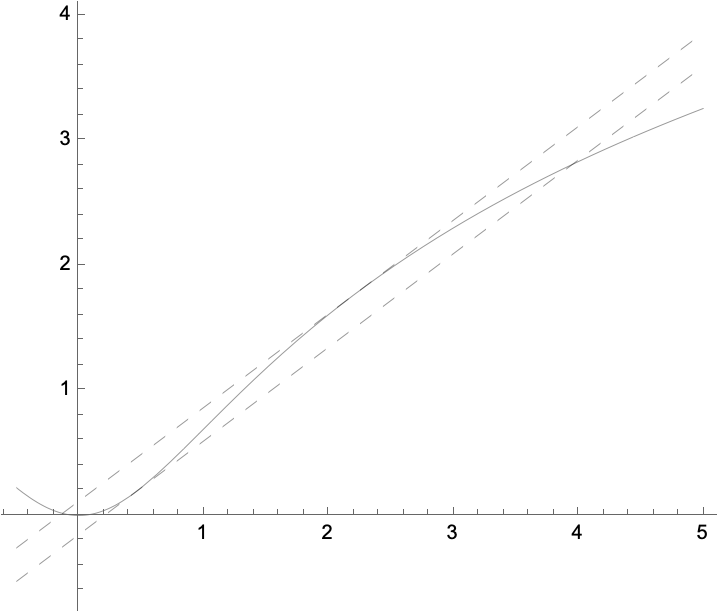
\includegraphics[width=\linewidth]{images/fig_2022A1.png}
\end{image}%
\tcblower
\end{figureptx}%
The equation \(f'(x) = a\) has exactly two solutions, at \(x=r_-\) and \(x=r_+\) for \(r_{\pm}\) as defined above. If we define \(g(x) = f(x)-ax\), then \(g'(r_\pm)=0\); \(g'\) is strictly decreasing on \((-\infty,r_-)\), strictly increasing on \((r_-,r_+)\), and strictly decreasing on \((r_+,\infty)\); and \(\lim_{x\to-\infty} g(x) = \infty\) while \(\lim_{x\to\infty} g(x) = -\infty\). It follows that \(g(x)=b\) has exactly one solution for \(b \lt g(r_-)\) or \(b>g(r_+)\), exactly three solutions for \(g(r_-)\lt b \lt g(r_+)\), and exactly two solutions for \(b = g(r_\pm)\). That is, \(y=ax+b\) intersects \(y=f(x)\) in exactly one point if and only if \(b\lt g(r_-)\) or \(b\gt g(r_+)\).%
\end{example}
\begin{example}{Example}{Riemann Sums and a challenging integral.}{example-example-riemann-limit}%
\index{Riemann Sum}%
Typical students often have more expertise in calculus than any other subject, but there are often gaps in their understanding of the topic.  One of them is Riemann sums and their role in integration.  A common textbook example is to start with a right Riemann sum of \(\int_0^1 x^5 \, dx\), \(\sum _{k=1}^n \left(\frac{k}{n}\right)^5 \cdot \frac{1}{n}\) and maybe disguise it to some extent.  Then ask for the limit as \(n\) goes to infinity.  Naturally the answer is simply the integral, \(\frac{1}{6}\).   The first part of solving B-1 in the 1976 Putnam was to identify a slightly more disguised example.%
\begin{quote}%
Evaluate%
\begin{equation*}
\lim_{n\to\infty} \frac{1}{n} \sum _{k=1}^n \left(\left\lfloor
\frac{2 n}{k}\right\rfloor -2
\left\lfloor
\frac{n}{k}\right\rfloor \right) 
\end{equation*}
%
\end{quote}
In this case, the function we are integrating is a bit more complicated, and integration is a second issue that isn't so straightforward.  The function is \(f(x)= \left\lfloor \frac{2}{x}\right\rfloor - 2 \left\lfloor \frac{1}{x}\right\rfloor\).%
\par
Evaluating the integral is non-trivial, but here is an overview.  When working with floor\slash{}ceiling functions, one trick  is to assume some condition that lets you work with an equality or inequality to infer more information.  In this case, we assume that  \(2\lfloor \frac{1}{x}\rfloor =2k\) for some positive integer \(k\).%
\begin{equation*}
\begin{split}
2\lfloor \frac{1}{x}\rfloor =2k &\Leftrightarrow  \lfloor \frac{1}{x}\rfloor=k\\
& \Leftrightarrow k \leq \frac{1}{x} \lt k +1 \\
& \Leftrightarrow \frac{1}{k+1} \lt x \leq \frac{1}{k}
\end{split}
\end{equation*}
%
\par
Therefore,%
\begin{equation*}
\begin{split}
k \leq \frac{1}{x} \lt k +1  &\Leftrightarrow 2k \leq \frac{2}{x} \lt 2k +2 \\
&\Leftrightarrow  \lfloor \frac{2}{x} \rfloor = 2k \textrm{ or } 2k + 1.
\end{split}
\end{equation*}
If \(\frac{1}{k+1} \lt x \leq \frac{2}{2k+1}\), we have \(\lfloor \frac{2}{x}\rfloor = 2k+1\); and if \(\frac{2}{2k+1} \lt x \leq \frac{1}{k}\), we have \([\frac{2}{x}] = 2k\).  Therefore,  on the interval \((\frac{1}{k+1}, \frac{1}{k}]\),%
\begin{equation*}
f(x)=\begin{cases} 1 & \textrm{if } \frac{1}{k+1} \lt x \leq \frac{2}{2k+1}\\
0 & \textrm{if } \frac{2}{2k+1} \lt x \leq \frac{1}{k}
\end{cases}
\end{equation*}
and \(\int_{\frac{1}{k+1}}^{\frac{1}{k}} f(x) dx = \frac{2}{2k+1}-  \frac{1}{k+1}\)%
\par
Finally, we have%
\begin{equation*}
\begin{split}
\int_{0}^{1} f(x) dx & = \sum_{k=1}^{\infty} \left( \frac{2}{2k+1}-  \frac{1}{k+1} \right) \\
&  = 2 \sum_{k=1}^{\infty} \left( \frac{1}{2k+1} - \frac{1}{2k+2} \right) \\
&  = 2 \left(\left( \sum_{k=1}^{\infty} (-1)^{k+1}\frac{1}{k}\right)  - (1-\frac{1}{2}) \right)\\
& = 2 \ln(2) - 1\\
& = \ln(4) - 1
\end{split}
\end{equation*}
%
\end{example}
\end{sectionptx}
%
%
\typeout{************************************************}
\typeout{Exercises 5.2 Exercises}
\typeout{************************************************}
%
\begin{exercises-section}{Exercises}{Exercises}{}{Exercises}{}{}{exercises-s-calculus-d}
\begin{divisionexercise}{1}{}{}{exercise-s-calculus-d-b}%
Let \(a,b,c,d,e \in \mathbb{R}\) such that \(a + \frac{b}{2} + \frac{c}{3} + \frac{d}{4} + \frac{e}{5} = 0\). Show that the polynomial \(a+bx+c x^2 +d x^3 +e x^4\) has at least one real zero. Note: In this context, \(e\) isn't the number we call \(e\), it's just an arbitrary real number.%
\par\smallskip%
\noindent\textbf{\blocktitlefont Solution}.\hypertarget{solution-s-calculus-d-b-b}{}\quad{}The pattern in the given equation should be recognized as the value of \(\int_0^1 \left(a+b x+c x^2+d x^3+e x^4\right) \, dx\).  If \(a=0\) we have a real root at zero. Otherwise, the only way for the integral to equal zero is for its graph to lie partially above and partially below the \(x\)-axis.  By the intermediate value theorem there must be a real root.%
\end{divisionexercise}%
\begin{divisionexercise}{2}{}{}{exercise-s-calculus-d-c}%
Prove that \(\sum _{k=1}^n \frac{1}{k}>\ln  (n+1)\)  for all \(n\geq 1\).%
\end{divisionexercise}%
\begin{divisionexercise}{3}{}{}{exercise-s-calculus-d-d}%
Generalizing the first part of this problem will lead to a characterization of the other parts.%
\begin{enumerate}[label=(\alph*)]
\item{}Find a partition \(\left\{t_0=1,t_1,t_2=2\right\}\) of \([1,2]\) that maximizes the lower Riemann sum that estimates the value of \(\int_1^2 \frac{1}{x} \, dx\) among all other partitions of size 2.%
\item{}Find a partition \(\left\{t_0=1,t_1,t_2,t_3=2\right\}\) of \([1,2]\) that maximizes the lower Riemann sum that estimates the value of \(\int_1^2 \frac{1}{x} \, dx\) among all other partitions of size 3.%
\item{}Find a partition \(\left\{t_0=1,t_1,t_2,\ldots , t_n=2\right\}\) of \([1,2]\) that maximizes the lower Riemann sum that estimates the value of \(\int_1^2 \frac{1}{x} \, dx\) among all other partitions of size \(n\).%
\end{enumerate}
%
\par\smallskip%
\noindent\textbf{\blocktitlefont Solution}.\hypertarget{solution-s-calculus-d-d-b}{}\quad{}We first generalize the problem of finding the maximizing partition of size 2 for the lower sum of \(\int_a^b \frac{1}{x} \, dx\)  for arbitrary real \(a, b\) where \(a \lt b\). The lower sum in this case is \(L=(t_1-a)\frac{1}{t_1} + (b-t_1)\frac{1}{b}\) differentiating \(L\) with respect to \(t_1\) and setting the derivative equal to zero yeilds a maximum at \(t_1=\sqrt{a b}\). Therefore the optimal partition in part (a) is \(\left\{1,\sqrt{2},2\right\}\). Our general observation can be used to argue that in the general case of \(n\) subintervals, the maximum lower sum must be attained with partition points that are powers of the \(n^{\textrm{th}}\) root of 2,%
\begin{equation*}
\left\{1,2^{1/n},2^{2/n},\dots, 2^{(n-1)/n)},2 \right\}.
\end{equation*}
With this partition, we can see that movement of any interior value will reduce the value of the lower sum by focusing in the interval that is partitioned by the moving value and it's two neighbors.%
\end{divisionexercise}%
\begin{divisionexercise}{4}{}{}{exercise-s-calculus-d-e}%
Determine the value of \(\lim _{n\to \infty }\sum _{k=1}^n \frac{k}{k^2+n^2}\)%
\par\smallskip%
\noindent\textbf{\blocktitlefont Hint}.\hypertarget{hint-s-calculus-d-e-b}{}\quad{}This is a limit of Reimann sums in disguise!%
\par\smallskip%
\noindent\textbf{\blocktitlefont Solution}.\hypertarget{solution-s-calculus-d-e-c}{}\quad{}%
\begin{equation*}
\begin{split}
\lim_{n\to \infty }\sum _{k=1}^n \frac{k}{k^2+n^2} &=\lim_{n\to \infty }\sum _{k=1}^n \frac{\frac{k}{n}}{(\frac{k}{n})^2+1}\frac{1}{n}\\
& = \int_0^1 \frac{x}{1+x^2} dx = \frac{\ln 2}{2}
\end{split}
\end{equation*}
%
\end{divisionexercise}%
\begin{divisionexercise}{5}{}{}{exercise-s-calculus-d-f}%
Let \(p(x)\) be a polynomial of even degree with a positive leading coefficient. Suppose \(p(x)\geq p''(x)	\) for every \(x\). Show that \(p(x) \geq  0\) for every \(x\).%
\par\smallskip%
\noindent\textbf{\blocktitlefont Solution}.\hypertarget{solution-s-calculus-d-f-b}{}\quad{}Indirect Proof:  Assume \(p(x)\lt 0\) for some \(x\).  The conditions of the problem implies that \(p(x)\) attains a minimum value at \(x=a\) for some \(a\).  Then \(p(a) \lt 0 \leq p''(a)\).  This contradicts the condition that \(p(x)\geq p''(x)\) for all \(x\).%
\end{divisionexercise}%
\begin{divisionexercise}{6}{}{}{exercise-s-calculus-d-g}%
If \(f\) is a differentiable function on \([0,1]\) such that \(f(0)=f(1)=0\), and if \(\int_0^1 \left| f'(x)\right| dx=1\), what can be said about \(f\left(\frac{1}{2}\right)\)? For example, is it possible that \(f\left(\frac{1}{2}\right)=0?\), or 1?, or \(\frac{1}{2}\)?, or -1?, or 2? Note: \emph{Differentiable} can be replaced with \emph{Absolutely Continuous}, but this is a somewhat more advanced property that isn't likely to be used in the Putnam (I could be wrong!)%
\end{divisionexercise}%
\begin{divisionexercise}{7}{}{}{exercise-s-calculus-d-h}%
Evaluate \(\int_{ 0}^{ \pi /2} \left(\sin ^2(\sin (x))+\cos ^2(\cos (x))\right) \, dx\).%
\end{divisionexercise}%
\begin{divisionexercise}{8}{}{}{exercise-s-calculus-d-i}%
For a positive constant \(k\), consider the region \(\mathcal{R}\) bounded by the line\(y = k x\) and the parabola \(y = x^2\). There is only one choice of \(k\) such that the solids obtained by revolving \(\mathcal{R}\) about the \(x\)-axis and the \(y\)-axis have the same volume. Find the value of this special choice of \(k\).%
\par\smallskip%
\noindent\textbf{\blocktitlefont Solution}.\hypertarget{solution-s-calculus-d-i-b}{}\quad{}The volume of revolution around the \(x\) axis is%
\begin{equation*}
\int_0^k \pi \left((k x)^2-x^4\right) \, dx=\frac{2\pi }{15}k^5\text{.}
\end{equation*}
Around the \(y\) axis we have (using shells)%
\begin{equation*}
\int _0^k2\pi  x\left(k x-x^2\right)dx=\frac{\pi }{6}k^4\text{.}
\end{equation*}
Therefore the special \(k\) is \(\frac{5}{4}\).%
\end{divisionexercise}%
\begin{divisionexercise}{9}{}{}{exercise-s-calculus-d-j}%
For which real numbers \(c\) is \(\frac{e^x+ e^{-x}}{2}\leq e^{c x^2}\) for all real \(x\)?%
\end{divisionexercise}%
\begin{divisionexercise}{10}{}{}{exercise-s-calculus-d-k}%
Let \(f(x)\) be a function such that \(f(1)=1\) and for \(x\geq 1\)%
\begin{equation*}
f'(x)=\frac{1}{x^2+ f(x)^2}\text{.}
\end{equation*}
Prove that \(\lim_{x\to \infty } f(x)\) exists and is less than \(1+\frac{\pi}{4}\).%
\end{divisionexercise}%
\begin{divisionexercise}{11}{}{}{exercise-s-calculus-d-l}%
Evaluate the infinite product \(\prod _{n=2}^{\infty } \frac{n^3-1}{n^3+1}\).%
\par\smallskip%
\noindent\textbf{\blocktitlefont Hint}.\hypertarget{hint-s-calculus-d-l-b}{}\quad{}Look at the ``partial products.''%
\par\smallskip%
\noindent\textbf{\blocktitlefont Solution}.\hypertarget{solution-s-calculus-d-l-c}{}\quad{}We first observe that \(\frac{n^3-1}{n^3+1} = \frac{(n-1)(n^2+n+1)}{(n+1)(n^2-n+1)}\), and that \(n^2-n+1 = (n-1)^2+(n-1)+1\).  The partial product up to \(n=M\) is%
\begin{equation*}
\Pi_M = \prod_{n=2}^M \frac{n^3-1}{n^3+1} = \prod_{n=2}^M \frac{n-1}{n+1}\cdot \frac{n^2+n+1}{(n-1)^2+(n-1)+1}= \frac{2}{3} \cdot \frac{M^2+M+1}{M(M+1)}.
\end{equation*}
The value of the infinite product is \(\lim_{M \rightarrow \infty} \Pi_M = 2/3\).%
\end{divisionexercise}%
\begin{divisionexercise}{12}{}{}{exercise-s-calculus-d-m}%
The minute hand on a watch is 8 mm long and the hour hand is 4 mm long. What is the rate of change (in \(mm/hr\)) of  the distance between the tips of the hands at one o’clock?%
\par\smallskip%
\noindent\textbf{\blocktitlefont Solution}.\hypertarget{solution-s-calculus-d-m-b}{}\quad{}(From MAA Northeast Section Competition, 2006) As depicted in \hyperref[figure-fig-sageplot-clock-hands]{Figure~{\xreffont\ref{figure-fig-sageplot-clock-hands}}}, let \(\theta\) and \(\ell\) be the angle between the hands and the distance between the tips of the hands, respectively.%
\begin{figureptx}{Figure}{Illustration of the variables in the clock problem}{figure-fig-sageplot-clock-hands}{}%
\begin{image}{0}{1}{0}%
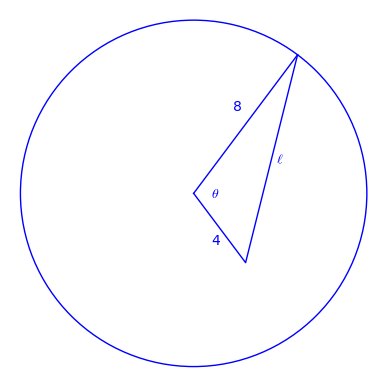
\includegraphics[width=\linewidth]{images/sageplot-clock-hands.png}
\end{image}%
\tcblower
\end{figureptx}%
The hour hand of a clock goes around once every 12 hours or, \(\frac{\pi}{6}\) radians per hour. The minute hand goes around once per hour, or at the rate of \(2 \pi\)  radians per hour. So the angle \(\theta\) between them (measuring clockwise from the minute hand to the hour hand) is changing at the rate of%
\begin{equation*}
\frac{d\theta}{dt} = \frac{\pi}{6}-2\pi \quad \textrm{rad/hr} 
\end{equation*}
%
\par
We want \(\frac{d\ell}{dt}\) at one o'clock, so we use the Law of Cosines establish a relationship between \(\theta\) and \(\ell\).%
\begin{equation}
\ell^2 = 4^2 + 8^2 -2\cdot 4\cdot 8\cdot cos\, \theta\label{men-clock-law-of-cosines}
\end{equation}
If we differentiate \hyperref[men-clock-law-of-cosines]{({\xreffont\ref{men-clock-law-of-cosines}})}  with respect to time  we get%
\begin{equation}
2 \ell \frac{d\ell}{dt} = -64(-sin\, \theta)\frac{d\theta}{dt}\label{men-clock-diff-of-law-of-cosines}
\end{equation}
At one o'clock, \(\theta = \pi/6\).   The Law of Cosines formula gives us the value of \(\ell\) at that time and  then  we can use \hyperref[men-clock-diff-of-law-of-cosines]{({\xreffont\ref{men-clock-diff-of-law-of-cosines}})} evaluated at \(\pi/6\) to get a final answer, which is \(-\frac{22 \pi}{3 \sqrt{5-2\sqrt{3}}}\)%
\par
Without a calculator, it's unlikely that you would ever be expected to approximate this number, but with that aid, we find that the tips of the hands are decreasing at a rate of 18.6 mm\slash{}h at 1:00.%
\end{divisionexercise}%
\begin{divisionexercise}{13}{}{}{exercise-s-calculus-d-n}%
Prove the following or provide a counterexample:  If \(\left\{f_n\right\}\) is a sequence of functions defined on the interval \([0,1]\) and that for each \(x\) in the interval \(\lim_{n\to \infty } f_n(x) = f(x)\),  then    \(\lim_{n\to \infty } \int_0^1 f_n(x) \, dx=\int_0^1 f(x)
\, dx\).%
\end{divisionexercise}%
\begin{divisionexercise}{14}{}{}{exercise-s-calculus-d-o}%
Evaluate \(\lim_{n \rightarrow \infty} \frac{1}{n}\ln{\left(\frac{(2n)!}{n! n^n}\right)}\).%
\par\smallskip%
\noindent\textbf{\blocktitlefont Hint}.\hypertarget{hint-s-calculus-d-o-b}{}\quad{}Think Riemann sum.%
\par\smallskip%
\noindent\textbf{\blocktitlefont Answer}.\hypertarget{answer-s-calculus-d-o-c}{}\quad{}\(\ln{4}-1\)%
\par\smallskip%
\noindent\textbf{\blocktitlefont Solution}.\hypertarget{solution-s-calculus-d-o-d}{}\quad{}We can simplify the logarithm in the limit first:%
\begin{equation*}
\ln\left(\frac{ (2 n)!}{n! n^n}\right) = \sum_{k=1}^n \ln{(\frac{n+k}{n})}
\end{equation*}
%
\par
The limit then becomes \(\lim_{n \rightarrow \infty} \frac{1}{n}\sum_{k=1}^n \ln{(1+\frac{k}{n})}\), which is the limit of Riemann sums for the integral \(\int_0^1 \ln{(1+x)}\,dx\), which evaluates to \(\ln{4}-1\).%
\end{divisionexercise}%
\begin{divisionexercise}{15}{}{}{exercise-s-calculus-d-p}%
Evaluate \(\lim_{n \rightarrow \infty} \frac{1}{n}\ln \left(\prod_{k=1}^{n} \frac{ n^2+k^2}{n^2}\right)\).%
\par\smallskip%
\noindent\textbf{\blocktitlefont Answer}.\hypertarget{answer-s-calculus-d-p-b}{}\quad{}\(-2+\frac{\pi }{2}+\log (2)\)%
\par\smallskip%
\noindent\textbf{\blocktitlefont Solution}.\hypertarget{solution-s-calculus-d-p-c}{}\quad{}%
\end{divisionexercise}%
\end{exercises-section}
\end{chapterptx}
%
%
\typeout{************************************************}
\typeout{Chapter 6 Number Theory}
\typeout{************************************************}
%
\begin{chapterptx}{Chapter}{Number Theory}{}{Number Theory}{}{}{chapter-c-number_theory}
\renewcommand*{\chaptername}{Chapter}
\begin{introduction}{}%
The starting point for number theory is the set of positive integers.  After developing basic arithmetic properties of this set, number theory goes in countless directions and is one of the richest of all mathematical subjects. Here, we touch on just a few key ideas.%
\end{introduction}%
%
%
\typeout{************************************************}
\typeout{Section 6.1 Primes and Relatively Prime Pairs}
\typeout{************************************************}
%
\begin{sectionptx}{Section}{Primes and Relatively Prime Pairs}{}{Primes and Relatively Prime Pairs}{}{}{section-sec-primes}
A prime are positive integer greater than one that are only divisible by one and itself. A fundamental theorem in number theory states that every positive integer greater than one is uniquely factorable as a product of one or more primes.%
\par
You should be familiar with the fact that there are an infinite number of primes, and if pressed, should be able to prove it.  There is only one even prime, 2. If we divide an odd prime by 4, the remainder will either be 1 or 3; so every odd prime has the form \(4k+1\) or \(4k+3\).  Here is a proof that there are an infinite number of primes of the second form. Suppose, to the contrary, that there are only a finite number of primes of the form \(4k+3\), and that they are  \(p_1=4k_1+3\), \(p_2=4k_2+3, \dots\), \(p_r=4k_r+3\).  Consider the integer \(Q= 4(p_1 \cdot p_2 \cdot \cdots \cdot p_r)+3\).  We observe that \(Q\) is an odd integer that is not divisible by any of the \(p_i\). It can be factored into a product of primes that are not in the set of \(p_i\) but the factors cannot all be of the form \(4k+1\) and so there is yet another prime of the form \(4k+3\) that was not accounted for in our list of such primes.  This contradiction implies that the set of these integer must be infinite.%
\par
We had just proven an instance of a more general theorem called \emph{Dirichlet's Theorem}, which states that if \(4k+3\) is replaced with \(\alpha k + \beta\) where \(\gcd(\alpha,\beta)=1\) we get the same conclusion, that there are an infinite number of primes of that form.%
\par
Individual positive integers are prime, but there is a related notion concerning \emph{pairs} of positive integers.%
\begin{definition}{Definition}{Relatively Prime.}{definition-sec-primes-f}%
\index{Relatively Prime}%
Let \(a\) and \(b\) be positive integers.  We say that they are relatively prime if their only common divisor is 1%
\end{definition}
Note that relatively prime integers need not be prime.%
\par
An important function on the positive integers is the Euler phi function.%
\begin{definition}{Definition}{Euler Phi Function.}{definition-sec-primes-i}%
\index{Euler Phi Function}%
\index{Euler Totiant Function}%
\label{notation-sec-primes-i-d}%
Let \(n\) be a positive integer. The value of \(\varphi(n)\) is the number of integers in the set \(\{1, 2,\dots ,n-1\}\) that are relatively prime to \(n\).%
\end{definition}
We will explore some the properties of this function in the exercises.%
\end{sectionptx}
%
%
\typeout{************************************************}
\typeout{Section 6.2 Residues}
\typeout{************************************************}
%
\begin{sectionptx}{Section}{Residues}{}{Residues}{}{}{section-c-number_theory-d}
The residues of integers modulo \(n\), \(n \geq 2\) are the remainders upon dividing integers by \(n\).  We start with a simple use of residues.%
\begin{example}{Example}{}{example-mod7}%
Show that \(n^2+ 1\) is divisible by 7 for no positive integer \(n\).%
\par
%
\begin{equation*}
\begin{split}
7 \mid (n^2+1) & \Leftrightarrow n^2 \equiv -1\pmod{7}\\
& \Leftrightarrow n^2 \equiv  6\pmod{7}\\
\end{split}
\end{equation*}
We can easily verify that for any \(n\), the residue of \(n^2\pmod{7}\) is never 6.%
\end{example}
\begin{example}{Example}{Chinese Remainder Theorem.}{example-example-crt}%
\index{Chinese Remainder Theorem}%
Let \(a, b\) be integers and \(m, n\) positive integers such that \(\gcd (m,n)=1\). Then there is a unique integer, \(x\), in the set \(\{0,1,2,\ldots , m n -1\}\) such that \(x\equiv a \pmod{m}\) and \(x\equiv b\pmod{n}\).%
\par
In order for an integer to satisfy the first conguence, we need \(x = a + m\cdot q_1\) for some integer \(q_1\).  Substitution into the second congruence gives us%
\begin{equation*}
a + m\cdot q_1\equiv b \pmod{n} \Rightarrow  m\cdot q_1\equiv b-a \pmod{n}
\end{equation*}
We know that since \(m\) and \(n\) are relatively prime, there exist integers \(s\) and \(t\) such that%
\begin{equation*}
m \cdot s + n \cdot t = 1  \Rightarrow   m \cdot s \equiv 1 \pmod{n}
\end{equation*}
and so%
\begin{equation*}
q_1\equiv s(b-a) \pmod{n}  \Rightarrow   x = a + m\cdot (s(b-a)+ n q_2)= x = a + m\cdot s\cdot(b-a)+ (m\cdot n) q_2 
\end{equation*}
for some integer \(q_2\). This set of solutions constitutes one residue class mod \(m \cdot n\) and so there is a unique solution in the desired set.%
\end{example}
\end{sectionptx}
%
%
\typeout{************************************************}
\typeout{Section 6.3 Euler's Theorem}
\typeout{************************************************}
%
\begin{sectionptx}{Section}{Euler's Theorem}{}{Euler's Theorem}{}{}{section-c-number_theory-e}
Euler's Theorem generalizes Fermat's Little Theorem.%
\begin{example}{Example}{}{example-power-mod-21}%
Compute \(5^{159} \pmod{21}\).%
\par
One solution to this problem is to observe that \(5^{159}\equiv 2 \pmod{3}\)  by applying Fermat's little theorem with \(p=3\); and then switching to calculations mod 7, find that \(5^{159}\equiv 6 \pmod{7}\).  We can then use the procedure outlined in the proof of the Chinese Remander Theorem to find that \(5^{159}\equiv 20 \pmod{21}\). Although this solution fine, it can be determined more efficiently with Euler's Theorem.%
\end{example}
\begin{theorem}{Theorem}{Euler's Theorem.}{}{theorem-c-number_theory-e-d}%
\index{Euler's Theorem}%
Let \(n\) be a positive integer greater than 1 and \(a\) a positive integer that is relatively prime to \(n\).  Then  \(a^{\varphi(n)} \equiv 1 \pmod{n}\)%
\end{theorem}
\begin{proof}{Proof}{}{proof-c-number_theory-e-d-d}
Consider the set \(U_n\) of all positive integers less than \(n\) that are relatively prime to \(n\). The cardinality of this set is \(\varphi(n)\).  We note that the function \(f\) on \(U_n\) defined by \(f(b) = a \cdot b \pmod{n}\) is a permutation of \(U_n\). Let \(X=\prod_{x \in U_n} x\). Then%
\begin{equation*}
\begin{split}
X  &= \prod_{x \in U_n} x =  \prod_{x \in U_n} f(x) \\
&\equiv  \prod_{x \in U_n} a\cdot x \pmod{n} \\
&\equiv  a^{\varphi(n)} \prod_{x \in U_n}  x \pmod{n} \\
& = a^{\varphi(n)} \cdot X
\end{split}
\end{equation*}
Multiplying both sides of the equivalence \(X \equiv a^{\varphi(n)} \cdot X \pmod{n}\) by the mod \(n\) inverse of \(X\) gets us the desired result.%
\end{proof}
\begin{example}{Example}{}{example-ex-euler-app}%
Revisiting the previous example, we can compute the value of \(\varphi(21)\) based on the exercise on \hyperlink{exercise-exercise-euler-phi}{Euler's Phi Function}:  \(\varphi(21)=\varphi(3)\cdot\varphi(7)=2 \cdot 6 = 12\).  This lets us reduce \(5^{159}\) to \(5^{3} \pmod{21}\), which reduces further to 20.%
\end{example}
\end{sectionptx}
%
%
\typeout{************************************************}
\typeout{Exercises 6.4 Problems}
\typeout{************************************************}
%
\begin{exercises-section}{Exercises}{Problems}{}{Problems}{}{}{exercises-c-number_theory-f}
\begin{introduction}{}%
Before starting these problems, you might want to review the statement of \hyperref[theorem-theorem-fermat-little]{Fermat's Little Theorem}.%
\end{introduction}%
\begin{divisionexercise}{1}{}{}{exercise-c-number_theory-f-c}%
We say that two positive rational numbers \(\frac{a}{b}\) and \(\frac{c}{d}\) are \emph{close} if \(a d - b c = \pm 1\).%
\begin{enumerate}[label=(\alph*)]
\item{}Prove that if \(\frac{a}{b}\) and \(\frac{c}{d}\) are close, then \(\frac{a+c}{b+d}\) is close to both \(\frac{a}{b}\) and \(\frac{c}{d}\).%
\item{}Find five rational numbers that are close to \(\frac{2}{7}\).%
\end{enumerate}
%
\end{divisionexercise}%
\begin{divisionexercise}{2}{Euler's Phi Function.}{}{exercise-exercise-euler-phi}%
Recall that \(\varphi(n)\) is the number of integers in the set \(\{1,2, \ldots  , n-1\}\) that are relatively prime to \(n\).%
\begin{enumerate}[label=(\alph*)]
\item{}Find and prove a formula for \(\varphi \left(p^k\right)\) if \(k\geq 1\) and \(p\) is prime.%
\item{}Prove that if \(a\) and \(b\) are relatively prime positive integers greater than \(1\), then  \(\varphi(a \cdot b)=\varphi(a) \cdot \varphi(b)\)%
\item{}Determine the value of \(\varphi(100!)\).%
\end{enumerate}
%
\end{divisionexercise}%
\begin{divisionexercise}{3}{}{}{exercise-c-number_theory-f-e}%
Show, without using a calculator, that \(2^9 + 2^{99}\) is divisible by 100.%
\end{divisionexercise}%
\begin{divisionexercise}{4}{}{}{exercise-c-number_theory-f-f}%
Find a Pythagorean triple that includes 2021 as a side length.%
\par\smallskip%
\noindent\textbf{\blocktitlefont Hint}.\hypertarget{hint-c-number_theory-f-f-b}{}\quad{}\(2025\) is a perfect square.%
\par\smallskip%
\noindent\textbf{\blocktitlefont Answer}.\hypertarget{answer-c-number_theory-f-f-c}{}\quad{}\((2021,180,2029)\)%
\par\smallskip%
\noindent\textbf{\blocktitlefont Solution}.\hypertarget{solution-c-number_theory-f-f-d}{}\quad{}Since \(2021 = 2025-4 = 45^2 - 2^2\), we can generate a Pythagorian triple from the general form \((b^2-a^2, 2 a b, b^2 + a^2)\) to get the triple \((2021,180,2029)\).%
\end{divisionexercise}%
\begin{divisionexercise}{5}{}{}{exercise-c-number_theory-f-g}%
Prove that some positive integral power of 17 ends in 0001 (base 10).%
\end{divisionexercise}%
\begin{divisionexercise}{6}{}{}{exercise-c-number_theory-f-h}%
For which positive integers \(n\) is there a sum of \(n\) consecutive integers that is a perfect square?%
\end{divisionexercise}%
\begin{divisionexercise}{7}{}{}{exercise-c-number_theory-f-i}%
Show that the equation \(x^2- y^2=2x y z\) has no solutions in the positive integers. Hint:%
\par\smallskip%
\noindent\textbf{\blocktitlefont Hint}.\hypertarget{hint-c-number_theory-f-i-b}{}\quad{}Consider a prime divisor of \(x y\).%
\end{divisionexercise}%
\begin{divisionexercise}{8}{}{}{exercise-c-number_theory-f-j}%
In \hyperref[example-example-riemann-limit]{Example~{\xreffont\ref{example-example-riemann-limit}}}, we showed an example of how to deal with floor\slash{}ceiling functions. Here is an problem from the 1983 Putnam that can be solved by starting with a similar approach.  We quote the problem verbatim, where \([x]\) was used for the floor function.%
\par
Let \(f(n)=n +[\sqrt{n}]\) where \([x]\) is the largest integer less than or equal to \(x\).  Prove that, for every positive integer \(m\), the sequence%
\begin{equation*}
m, f(m), f(f(m)), f(f(f(m))), \dots
\end{equation*}
contains at least one square of an integer.%
\par\smallskip%
\noindent\textbf{\blocktitlefont Hint}.\hypertarget{hint-c-number_theory-f-j-b}{}\quad{}Assume \(m = k^2 + j\) where \(0 \leq j \leq 2k\).%
\par\smallskip%
\noindent\textbf{\blocktitlefont Solution}.\hypertarget{solution-c-number_theory-f-j-c}{}\quad{}(Based on a solution by Steven Oslan)  Let \(m = k^2 + j\) where \(0 \leq j \leq 2k\). We consider this the \((k,j)\) position, with an excess of \(j\).  Consider the following three cases depending on the current position.%
\begin{itemize}[label=\textbullet]
\item{}Case 0: \(j=0\). In this case, we are done!%
\item{}Case 1: \(1 \leq j \leq k\).  \(f(m)=k^2 + j + k\); so \(f(m)\) places us in position \((k,j+k)\) which is Case 2 since  \(k+1 \leq j +k \leq 2k.\)%
\item{}Case 2: \(k+1 \leq j \leq 2k\).   In this case, \(f(m)=k^2 + j + k = = (k+1)^2 + j-k-1\), and \(0 \leq j-k-1 \leq k-1\). This puts us into either Case 0 or Case 1.%
\end{itemize}
Notice that applying \(f\) successively bounces us between cases 1 and 2 until we are sent into Case 0.  Starting in Case 1 with an excess of \(j\), the excess increases by \(k\) in the next application of \(f\) but then the following application of \(f\) decreases the excess by \(k+1\), so that these two application reduce the excess by 1, to \(j-1\).  Therefore, \(2 j\) steps after being in case 1, we are done.%
\end{divisionexercise}%
\begin{divisionexercise}{9}{}{}{exercise-c-number_theory-f-k}%
Consider the sequence \(T\) defined by \(T_1=2\) and \(T_{n+1}=T_n^2-T_n+1\) when \(n \geq 1\). Prove that if \(m \neq n\) then \(T_m\) and \(T_n\) have no common factor greater than \(1\).%
\par\smallskip%
\noindent\textbf{\blocktitlefont Hint}.\hypertarget{hint-c-number_theory-f-k-b}{}\quad{}Look closely at the first few terms of the sequence.  A plausible formula may be suggested.%
\end{divisionexercise}%
\begin{divisionexercise}{10}{}{}{exercise-c-number_theory-f-l}%
What is the sum of the digits of the sum of the digits of the sum of the digits of \(4444^{4444}\)?%
\par\smallskip%
\noindent\textbf{\blocktitlefont Solution}.\hypertarget{solution-c-number_theory-f-l-b}{}\quad{}Let \(S(n)\) be the sum of the base 10 digits of \(n\).  Since  \(10^k \equiv 1 \pmod{9}\) for all \(k \geq 0\),%
\begin{equation*}
s \equiv S(n) \equiv S^{2}(n) \equiv S^{3}(n) \pmod{9}\text{,}
\end{equation*}
we can determine the residue of the desired value mod 9 by identifying the pattern in the powers of \(4444\).%
\begin{equation*}
\begin{split}
4444^1 \equiv 7 \pmod{9}\\
4444^2 \equiv 4 \pmod{9}\\
4444^3 \equiv 1 \pmod{9}\\
4444^4 \equiv 7 \pmod{9}
\end{split}
\end{equation*}
The powers are cyclic with period 3, and so \(S^3(4444^{4444}) \equiv 7 \pmod{9}\).%
\par
Now we need to do some estimation.  First we bound  \(S(4444^{4444})\).%
\begin{equation*}
4444^{4444} \lt 1000^{5000} = 10^{15000} \Rightarrow S(4444^{4444}) \leq 9\cdot 15000 = 135000
\end{equation*}
The sum of the digits of \(S(4444^{4444})\) is no more than the sum of the digits of 13499, or 35. Therefore the sum of the digits of  \(S(S(4444^{4444}))\) is bounded by the sum of digits of integers that are less than or equal to 35.  The maximum is then the sum of digits of 29, or 11.   The bound of 11 on \(S^3(4444^{4444})\) combined with the fact that it is congruent to 7 mod 9 implies that our answer is 7.%
\end{divisionexercise}%
\begin{divisionexercise}{11}{}{}{exercise-c-number_theory-f-m}%
Let \(n\) be an integer greater than or equal to four.  Each of the numbers \(x_1\), \(x_2\), ..., \(x_n\) equal 1 or -1, and%
\begin{equation*}
\begin{split}
x_1x_2x_3x_4+x_2x_3x_4x_5+x_3x_4x_5x_6+\cdots+x_{n-3}x_{n-2}x_{n-1}x_n+\\
x_{n-2}x_{n-1}x_nx_1+x_{n-1}x_nx_1x_2+x_nx_1x_2x_3=0
\end{split}\text{.}
\end{equation*}
Prove that \(n\) is divisible by 4.%
\par\smallskip%
\noindent\textbf{\blocktitlefont Hint}.\hypertarget{hint-c-number_theory-f-m-b}{}\quad{}Use odd\slash{}even parity twice.%
\par\smallskip%
\noindent\textbf{\blocktitlefont Solution}.\hypertarget{solution-c-number_theory-f-m-c}{}\quad{}The fact that each term equal \(\pm 1\) and they balance to 0 implies that \(n\) must be even.  To infer a further factor of 2 in \(n\) we note that if the terms in the given sum are multiplied the result is \((-1)^{n/2}\).   But if we look at this product closely we see that each of the \(x_i\)'s appears four times, so the product must be 1.  Therefore \(n/2\) is even and we are done.%
\end{divisionexercise}%
\begin{divisionexercise}{12}{}{}{exercise-c-number_theory-f-n}%
Find all positive integers \(n\) such that \(n!\) ends in exactly 1000 zeros.%
\par\smallskip%
\noindent\textbf{\blocktitlefont Hint}.\hypertarget{hint-c-number_theory-f-n-b}{}\quad{}Count the factors of 5 in \(n!\).%
\par\smallskip%
\noindent\textbf{\blocktitlefont Solution}.\hypertarget{solution-c-number_theory-f-n-c}{}\quad{}The number of zeros that appear at the end of \(n!\) is equal to the total number of factors of 5 in \(n!\).  We also need factors of 2, but there are an excess of those as we increase \(n\).  The number of factors of 5 in \(n!\) is%
\begin{equation*}
z(n)=\sum_{k=1}^{\infty} \lfloor \frac{n}{5^k} \rfloor
\end{equation*}
The first term of this sum is \(800\) when \(n=4000\) and \(1000\) when \(n=5000\), so direct calculation starting at \(4000\) would seem to make sense. In fact \(z(4005)=1000\) Therefore integers from \(4005\) to \(4009\) are what we are looking for. %
\end{divisionexercise}%
\begin{divisionexercise}{13}{}{}{exercise-c-number_theory-f-o}%
Prove that among any three distinct integers we can find two, say \(a\) and \(b\), such that the number \(a^3b - a b^3\) is a multiple of 10.%
\par\smallskip%
\noindent\textbf{\blocktitlefont Solution}.\hypertarget{solution-c-number_theory-f-o-b}{}\quad{}No matter which two integers are selected, \(f(a,b)=a^3b - a b^3=a b (a-b)(a+b)\) will be even.  If \(a\) and \(b\) are odd, their sum will be even. Less obvious is whether  \(f(a,b)\) will be divisible by 5. Not every pair produces a multiple of 5, such as \(f(2,1)=6\).  If any one of the given integers is a multiple of 5, we are done, so assume we have no multiples of five given.  This means that each of the three integers can be mapped to one of the two sets \(\{1,4\}\) or \(\{2,3\}\) according to which set its residue mod 5 belongs.   By the pigeonhole principle, there are two integers, \(a\) and \(b\), that map to the same set.  If their residues are equal, then they differ by a multiple of 5 and if their residues are different, their sum is a multiple of 5.  Either way, \(f(a,b)\) be a multiple of 5.%
\end{divisionexercise}%
\begin{divisionexercise}{14}{}{}{exercise-c-number_theory-f-p}%
Prove that for any positive integer \(n\) there exists an \(n\)-digit number divisible by \(2^n\) and containing only the digits 2 and 3.%
\par\smallskip%
\noindent\textbf{\blocktitlefont Solution}.\hypertarget{solution-c-number_theory-f-p-b}{}\quad{}(Proof by induction) Let \(p(n)\) be the statement that there exists an \(n\) digit integer with base 10 representation using only digits 2 and 3 that is divisible by \(2^n\).  The basis, \(p(1)\) is clearly true since 2 satisfies the conditions.%
\par
Assume \(p(n)\) is true for some \(n \ge 1\), and \(a=2^n b\) satisfies the conditions in that case.  If \(b\) is odd, then \(3\cdot 10^n + a = 2^n(5^n\cdot 3 + b)\) prepends \(a\) with the digit 3 and is divisible by \(2^{n+1}\) since \(5^n\cdot 3 + b\) is even.  If \(b\) is even, then \(2\cdot 10^n + a = 2^{n+1}\cdot 5^n + 2^n\cdot b\) satisfies the desired condition since both terms of the sum are divisible by \(2^{n+1}\) and 2 is prepended to \(a\).%
\par
A second proof, attributed to Nicholas Raymond, is to note that there are \(2^n\) different positive integers with \(n\) digits, each 2 or 3.  We can prove that there is a one-to one correspondence between these integers and the residues \(\mod{2^n}\), \(\{ 0, 1, 2, \dots, 2^{n-1} \}\).  This implies that exactly one of these integers is congruent to 0 and so must be divisible by \(2^n\).%
\end{divisionexercise}%
\begin{divisionexercise}{15}{}{}{exercise-c-number_theory-f-q}%
(2019 Putnam B-1) Denote by \(\mathbb{Z}^2\) the set of all points \((x,y)\) in the plane with integer coordinates. For each integer \(n \geq 0\), let \(P_n\) be the subset of \(\mathbb{Z}^2\) consisting of the point \((0,0)\) together with all points \((x,y)\) such that \(x^2 + y^2 = 2^k\) for some integer \(k \leq n\). Determine, as a function of \(n\), the number of four-point subsets of \(P_n\) whose elements are the vertices of a square.%
\par\smallskip%
\noindent\textbf{\blocktitlefont Solution}.\hypertarget{solution-c-number_theory-f-q-b}{}\quad{}Note that \(P_0 = \{ (0,0), (1,0), (-1,0), (0,1), (0,-1)\}\).  For \(n \geq 1\), let  \(P_n' =P_n - P_{n-1}\).  First, prove that if \(n\) is odd, then \(P_n' = \{(\pm 2^{(n-1)/2},\pm 2^{(n-1)/2})\}\); and if \(n\) is even, \(P_n' = \{(\pm 2^{n/2},0),(0,\pm 2^{n/2})\}\)..  Both cases can be proven by induction.%
\par
Let \(S(n)\) be the number of four point subsets of \(P_n\) that are the vertices of a square.  Note that \(S(0)=1\).  For \(n \geq 1\) notice that by adding \(P_{n}'\) to \(P_{n-1}\) we get an additional five squares - the square formed by \(P_{n}'\), and the four squares that make up a quarter of that large square. Therefore \(S(n) = 5 + S(n-1)\) and so \(S(n)=5n + 1\).%
\end{divisionexercise}%
\begin{divisionexercise}{16}{}{}{exercise-c-number_theory-f-r}%
Does there exist a positive integer with the property that the sum of the (base 10) digits of it’s square is equal to 100?  If so, find one. What if 100 is replaced with 2019?%
\par\smallskip%
\noindent\textbf{\blocktitlefont Hint}.\hypertarget{hint-c-number_theory-f-r-b}{}\quad{}Before launching into a search of whether a number that we seek exists, it is worth considering the problem mod 9 since the sum of the digits of a positive integer is congruent mod 9 to the integer itself.   Controlling the digits of a square is easiest with certain special numbers.   One such type number is \(10^k-d\) where \(k\) is a positive integer and \(d\) is a digit.%
\par\smallskip%
\noindent\textbf{\blocktitlefont Solution}.\hypertarget{solution-c-number_theory-f-r-c}{}\quad{}Observe that \((10^k - 2)^2\) is an integer whose digits consist of \(k\) nines, a single six, some zeros, and then a 4.   Therefore we get the number when \(k=11\).  Following the pattern of digits in \(11^2\), \(111^2\), \(1111^2, \dots\) doesn't quite get what we want, but prepending an integer with all ones with a 10 works.   Since \(2019 \equiv 2 \pmod{9}\) no square can have sum of digits equal to 2019.%
\end{divisionexercise}%
\end{exercises-section}
\end{chapterptx}
%
%
\typeout{************************************************}
\typeout{Chapter 7 Inequalities}
\typeout{************************************************}
%
\begin{chapterptx}{Chapter}{Inequalities}{}{Inequalities}{}{}{chapter-c-inequalities}
\renewcommand*{\chaptername}{Chapter}
\begin{introduction}{}%
As with most topics, we could spend a whole semester on inequalities.  Here we concentrate on Jensen Inequality,  the relationship between the different means, and the Cauchy-Bunyakovsky-Schwarz inequality. We also introduce Young's inequality as optional reading.%
\end{introduction}%
%
%
\typeout{************************************************}
\typeout{Section 7.1 Jensen's Inequality}
\typeout{************************************************}
%
\begin{sectionptx}{Section}{Jensen's Inequality}{}{Jensen's Inequality}{}{}{section-c-inequalities-c}
\index{Convex Function}%
In calculus one hears of concave upward functions, which are function with a positive second derivative.  Functions of this type are also called convex functions.  But convex function is more general than that.  A function is convex if any line segment connecting two points on its graph lies above the graph of the function. This translates to the more formal definition that \(f\) is convex on an interval \([a,b]\), if for \(a \leq t_1 \lt t_2 \leq b\), and \(0 \leq \lambda \leq 1\) it is true that%
\begin{equation*}
f(\lambda t_1 + (1-\lambda) t_2) \leq \lambda f(t_1)+(1-\lambda)f(t_2).
\end{equation*}
This is the simplest form of Jensen's inequality. A more general inequality follows.%
\begin{theorem}{Theorem}{Jensen's Inequality.}{}{theorem-c-inequalities-c-d}%
\index{Jensen's Inequality}%
If \(f\) is convex on an interval \([a,b]\), then for \(a \leq t_1 \lt t_2 \lt \cdots \lt t_n \leq b\), and positive real numbers \(\lambda_1, \lambda_2, \dots, \lambda_n\) such that \(\sum_{k=1}^n \lambda_k =1\),%
\begin{equation*}
f\left(\sum_{k=1}^n \lambda_k t_k \right) \leq  \sum_{k=1}^n \lambda_k  f(t_k).
\end{equation*}
%
\end{theorem}
\index{Concave Function}Although Jensen's inequality is most frequently stated for convex function, it also has a counterpart for concave functions, for which line segments lie below the graph.  The only change is to switch the inequality symbol.%
\end{sectionptx}
%
%
\typeout{************************************************}
\typeout{Section 7.2 Means}
\typeout{************************************************}
%
\begin{sectionptx}{Section}{Means}{}{Means}{}{}{section-s-means}
\index{Arithmetic Mean}%
\index{Geometric Mean}%
There are many means on a finite number of nonnegative real numbers.  Here we focus on a few of the most common.  The \emph{arithmetic mean} of \(n\) numbers, or what we often call their average, is their sum divided by \(n\).  The \emph{geometric mean} is computed by taking \(n^{th}\) root of their product.  We establish the relationship between these two means in the following theorem.%
\begin{theorem}{Theorem}{The AM\slash{}GM inequality.}{}{theorem-s-means-e}%
\index{AM\slash{}GM inequality}%
Assume \(n \geq 2\).  If \(a_i\), \(i = 1, 2, \dots, n\) are non-negative real numbers, then%
\begin{equation*}
\left(a_1 a_2\cdots  a_n\right)^{1/n}\leq  \frac{a_1+a_2+\cdots +a_n}{n}
\end{equation*}
with equality if and only if all the \(a_i\) are equal.%
\end{theorem}
\begin{proof}{Proof}{}{proof-s-means-e-d}
A proof by induction, but a somewhat unconventional one taken from \hyperlink{biblio-biblio-aigner}{[{\xreffont 1}]}. If \(n \ge 2\) then let \(P(n)\) the inequality for \(n\) numbers.  Instead of going forward one step at a time starting at 2, we start at 2 and prove the two general implications  \(P(n)\Rightarrow P(n-1)\)  and \(P(n)\Rightarrow P(2n)\).  After proving the basis, \(n=2\), we can apply these two implications in several ways; for example, we can infer the truth for values \(4, 3, 8, 7, 6, 5, 16, 15, 14, \dots, 9, 32, 31, 30 \dots\).%
\par
We leave the proof for \(n=2\) as an exercise.  Then we assume that for some \(n \geq 2\), the inequality is true and then assume we have \(2n\) numbers.%
\begin{equation*}
\begin{split}
\prod_{k=1}^{2n} a_k &=\left(\prod_{k=1}^{n} a_k \right)\left(\prod_{k=n+1}^{2n} a_k  \right) \\	
& \leq \left(\sum_{k=1}^{n} \frac{a_k}{n} \right)^n \left(\sum_{k=n+1}^{2n} \frac{a_k}{n} \right)^n \quad \textrm{ by }P(n)\textrm{, twice}\\
& \leq \left(\frac{\sum_{k=1}^{2n} \frac{a_k}{n}}{2}\right)^{2n} \quad \textrm{ by }P(2)\\
& = \left(\frac{\sum_{k=1}^{2n} a_k}{2n}\right)^{2n} 
\end{split}
\end{equation*}
Now if \(n \ge 3\) we assume \(P(n)\) is true and we have \(n-1\) numbers. We append the arithmetic mean of these numbers, \(A = \sum_{k=1}^{n-1} \frac{a_k}{n-1}\), to our collection and apply \(P(n)\):%
\begin{equation*}
\begin{split}
\left(\prod_{k=1}^{n-1} a_k\right)A & \leq \left(\frac{\left(\sum_{k=1}^{n-1} a_k\right) + A}{n}\right)^n\\
& = \left( \frac{(n-1)A + A}{n} \right)^n = A^n
\end{split}
\end{equation*}
dividing by \(A\), we get \(\left(\prod_{k=1}^{n-1} a_k\right) \leq A^{n-1} = \left(\frac{\sum_{k=1}^{n-1} a_{k}}{n-1}\right)^{n-1}\).%
\end{proof}
The AM\slash{}GM inequality can be used in optimization.  Here is an example.%
\begin{example}{Example}{}{example-s-means-g}%
Problem:  If \(x\) and \(y\) are positive real numbers such that \(x+2y=1\), what is the largest possible value of \(x^2 y\)?%
\par
A first attempt at this problem might be to write this:%
\begin{equation*}
x^2 y \leq  \left( \frac{x + x + y}{3} \right)^3
\end{equation*}
However, it's \(x+2y\), not \(2x + y\) that is invariant. The objective function needs to be adjusted with the right constants.%
\begin{equation*}
\begin{split}
x^2 y &= \frac{1}{4} \cdot x\cdot x\cdot (4 y) \\
&\leq  \frac{1}{4} \left( \frac{2(x+2y)}{3} \right)^3\\
& = \frac{1}{4} \left( \frac{2}{3} \right)^3 = \frac{2}{27} 
\end{split}
\end{equation*}
with equality when \(x=4y\), which implies that the maximum is attained when \(y=\frac{1}{6}\) and \(x=\frac{2}{3}\).%
\end{example}
In the exercises we examine the harmonic mean and how it is related to the arithmetic and geometric means.%
\end{sectionptx}
%
%
\typeout{************************************************}
\typeout{Section 7.3 The CBS Inequality}
\typeout{************************************************}
%
\begin{sectionptx}{Section}{The CBS Inequality}{}{The CBS Inequality}{}{}{section-c-inequalities-e}
The Cauchy-Bunyakovsky-Schwarz, or CBS, inequality has both discrete and continuous versions.  The real discrete version follows.%
\begin{theorem}{Theorem}{Cauchy-Bunyakovsky-Schwarz Inequality.}{}{theorem-c-inequalities-e-c}%
\index{Cauchy-Bunyakovsky-Schwarz Inequality}%
\index{CBS Inequality}%
If \(x\) and \(y\) are vectors in \(\mathbb{R}^n\), then%
\begin{equation}
\left(\sum _{i=1}^n x_i y_i\right)^2\leq \left(\sum _{i=1}^n x_i^2\right)\left(
\sum _{i=1}^n y_i^2\right)\label{men-eq-cbs}
\end{equation}
with equality if and only if the two vectors are scalar multiples of one another.%
\end{theorem}
\begin{proof}{Proof}{}{proof-c-inequalities-e-c-e}
There are many proofs of this inequality.  Here is a brief one from \hyperlink{biblio-biblio-aigner}{[{\xreffont 1}]}. We observe that the inequality can be express more compactly using norm and inner product notation as \((x, y)^2 \leq \left\Vert x \right\Vert^2 \left\Vert y \right\Vert^2 \).%
\par
We can assume that both \(x\) and \(y\) are nonzero vectors, for otherwise the inequality is obvious.  Let \(\alpha\) be a real variable, and consider the square of the norm of the vector \(\alpha x + y\).  If \(x\) and \(y\) are linearly independent, then \(\left\Vert \alpha x + y\right\Vert \gt 0\).  We expand the square of this norm:%
\begin{equation*}
\begin{split}
\left\Vert \alpha x + y \right\Vert^2 &= (\alpha x + y,\alpha x + y)\\
&  = \alpha^2 \left\Vert x \right\Vert^2 + 2 \alpha (x, y) + \left\Vert y \right\Vert^2
\end{split}
\end{equation*}
This quadratic polynomial in \(\alpha\) has no real roots and so the discriminant, \(4 (x, y)^2 - 4\left\Vert x \right\Vert^2 \left\Vert y \right\Vert^2 \lt 0\), which implies CBS.%
\par
If  \(x\) and \(y\) are linearly dependent, we get equality since the discriminant would equal zero.%
\end{proof}
\begin{example}{Example}{}{example-c-inequalities-e-d}%
From \hyperlink{biblio-biblio-steele-2004}{[{\xreffont 15}]}, This illustrates the ``1-Trick.''  Show that for each real sequence \(x_1, x_2, \dots, x_n\) one has%
\begin{equation*}
x_1 + x_2 + \cdots + x_n \leq \sqrt{n} \left(x_1^2 + x_2^2 + \cdots + x_n^2\right)^{1/2} 
\end{equation*}
%
\par
As the title suggest, we can derive this quite simply by taking \(y_k = 1\) for all \(k\) in \hyperref[men-eq-cbs]{({\xreffont\ref{men-eq-cbs}})}.%
\end{example}
\end{sectionptx}
%
%
\typeout{************************************************}
\typeout{Section 7.4 Young's Inequality}
\typeout{************************************************}
%
\begin{sectionptx}{Section}{Young's Inequality}{}{Young's Inequality}{}{}{section-c-inequalities-f}
Given positive numbers  and  whose reciprocals add up to one, the product  of two positive real numbers  and  is less than or equal to a weighted sum of \(p^{th}\) and \(q^{th}\) powers  of \(a\) and \(b\).%
\begin{theorem}{Theorem}{Young's inequality.}{}{theorem-c-inequalities-f-c}%
\index{Young's inequality}%
If \(a\) and \(b\) are nonnegative real numbers and \(p\) and \(q\) are positive real numbers such that \(\frac{1}{p} + \frac{1}{q} = 1\), then%
\begin{equation*}
a\cdot b \leq \frac{a^{p}}{p} + \frac{b^{q}}{q},
\end{equation*}
with equality if and only if \(f(a)=b\).%
\end{theorem}
\begin{proof}{Proof}{}{proof-c-inequalities-f-c-d}
The proof follows from the following more general inequality, where \(f(x)=x^{p-1}\).%
\end{proof}
\begin{theorem}{Theorem}{}{}{theorem-c-inequalities-f-d}%
If \(f\) is a strictly increasing function on the positive real numbers, \(f(0)=0\), and \(a\) and \(b\) are positive real numbers, then%
\begin{equation*}
a b \leq \int_0^a f(x) \, dx +\int_0^b f^{-1}(y) \, dy
\end{equation*}
%
\end{theorem}
\begin{proof}{Proof}{}{proof-c-inequalities-f-d-b}
If \(b=f(a)\), then the rectangle \([0,a]\times[0,b]\) is divided into two regions, the region below the curve \(y=f(x)\), and the region to the left of \(x = f^{-1}(y)\).  The sum of the two integrals is exactly equal to the area, \(a\cdot b\).  If \(f(a) \gt b\), the region whose area  \(\int_0^b f^{-1}(y) \, dy\) computes is contained within the rectangle, but the region whose area \(\int_0^a f(x) \, dx\) computes spills outside the rectangle, making the inequality a strict one.  This case is illustrated by \hyperref[figure-figure-young]{Figure~{\xreffont\ref{figure-figure-young}}}.  In the other case, where \(f(a) \lt b\), the excess area that makes the inequality a strict one is accounted for by \(\int_0^b f^{-1}(y) \, dy\).%
\end{proof}
This interactive SageMath expression illustrates the proof above for the case where \(f(x)=x^{p-1}\), \(p \gt 1\).%
\begin{sageinput}
@interact()
def young(a=(2,(1/4,3)),b=(3/2,(1/4,3)),p=(7/4,(1/8,5,1/8))):
    pl=plot(x^(p-1),(x,0,a),fill='min',
                           fillcolor='red',ticks=[[],[]])
    pl+=plot(x^(p-1),(x,0,b^(1/(p-1))),fill='max',
                           fillcolor='blue')
    pl+=text('a='+str(n(a,3)),[a,-0.1])
    pl+=text('b='+str(n(b,3)),[-0.1, b])
    pl+=text('separating curve is $y=x^{p-1}$',[1.3*a,0.5*b])
    show(pl,aspect_ratio=1)
\end{sageinput}
\begin{sageoutput}

\end{sageoutput}
The output from the SageMath expression above is a dynamic version of this image:%
\begin{figureptx}{Figure}{A visualization of the derivation of Young's Inequality}{figure-figure-young}{}%
\begin{image}{0}{1}{0}%
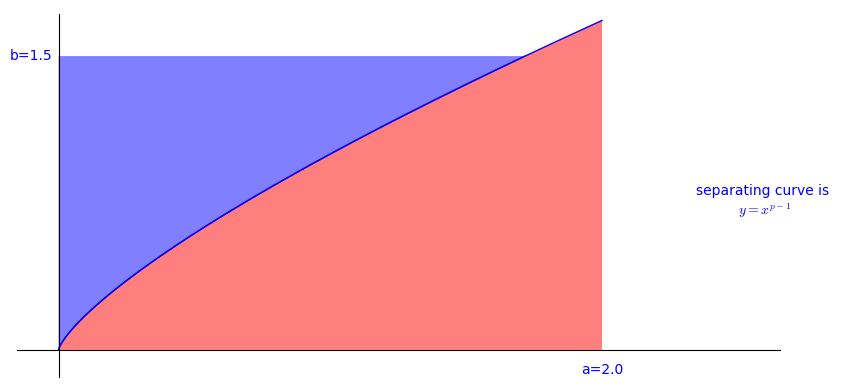
\includegraphics[width=\linewidth]{images/young.png}
\end{image}%
\tcblower
\end{figureptx}%
\end{sectionptx}
%
%
\typeout{************************************************}
\typeout{Exercises 7.5 Problems}
\typeout{************************************************}
%
\begin{exercises-section}{Exercises}{Problems}{}{Problems}{}{}{exercises-c-inequalities-g}
\begin{divisionexercise}{1}{}{}{exercise-c-inequalities-g-b}%
Let \(a\) and \(b\) be positive real numbers. Prove that \(\sqrt{a b}\leq \frac{a+b}{2}\)  with equality if and only if \(a=b\).%
\end{divisionexercise}%
\begin{divisionexercise}{2}{}{}{exercise-c-inequalities-g-c}%
\index{Harmonic Mean}%
How does the \terminology{harmonic mean} of two nonnegative real numbers, \(a\) and \(b\),  \(\frac{2}{\frac{1}{a}+\frac{1}{b}}\), compare with their geometric and arithmetic means?%
\par\smallskip%
\noindent\textbf{\blocktitlefont Hint}.\hypertarget{hint-c-inequalities-g-c-c}{}\quad{}Select two simple numbers and compute their harmonic, geometric and arithmetic means.  If there is going to be consistency, you know what it should be.  Then the hard work is to prove it!%
\end{divisionexercise}%
\begin{divisionexercise}{3}{}{}{exercise-c-inequalities-g-d}%
\index{Quadratic Mean}%
Let \(a\) and \(b\) be positive real numbers. Identify and prove the relationship between their \terminology{Quadratic Mean}, \(\sqrt{\frac{a^2 + b^2}{2}}\), and their other means.%
\end{divisionexercise}%
\begin{divisionexercise}{4}{}{}{exercise-c-inequalities-g-e}%
There are many possible proofs of the AM\slash{}GM inequality.  One is a direct application of Jensen's Inequality for concave functions.  Prove it that way.%
\par\smallskip%
\noindent\textbf{\blocktitlefont Hint}.\hypertarget{hint-c-inequalities-g-e-b}{}\quad{}There is a fairly obvious choice for \(f\).%
\end{divisionexercise}%
\begin{divisionexercise}{5}{}{}{exercise-c-inequalities-g-f}%
An express delivery service restricts the size of packages it will accept.  Packages cannot exceed 18 inches in length plus girth, i. e., \(\text{length}+2\times\text{width} +2\times \text{height}\leq 18\).  Find the maximum volume of an acceptable package.%
\par\smallskip%
\noindent\textbf{\blocktitlefont Solution}.\hypertarget{solution-c-inequalities-g-f-b}{}\quad{}By the GM\slash{}AM inequality,%
\begin{equation*}
\begin{split}
(l \cdot 2w \cdot 2h)^{1/3} & \leq \frac{l+2w+2h}{3}\leq \frac{18}{3}\\
& \Rightarrow (4 l w h)^{1/3} \leq 6\\
& \Rightarrow  l w h \leq 54
\end{split}
\end{equation*}
with equality when \(l = 2w = 2h = 6\). Thus, the maximum, 54, is attained when \(l=6\) and \(w=h=3\).%
\par
One could also argue, using calculus, that since the quantities \(l\), \(2w\), and \(2h\)  can be though of as edge lengths of a rectangular prism, its volume is maximized by a cube. This implies \(l = 2w = 2h = 6\).%
\end{divisionexercise}%
\begin{divisionexercise}{6}{}{}{exercise-c-inequalities-g-g}%
Let \(a_1, a_2, \ldots, a_{n }\) be positive, with sum 1.    Show that \(\sum _{i=1}^n a_i^2\geq \frac{1}{n}\)  and   \(\sum _{i=1}^n
a_i^4\geq \frac{1}{n^3}\)%
\par\smallskip%
\noindent\textbf{\blocktitlefont Hint}.\hypertarget{hint-c-inequalities-g-g-b}{}\quad{}Extend the ``one trick.''%
\par\smallskip%
\noindent\textbf{\blocktitlefont Solution}.\hypertarget{solution-c-inequalities-g-g-c}{}\quad{}The CBS inequalty using the ``one trick'' implies%
\begin{equation*}
1=\sum_{k=1}^n a_k \cdot 1 \leq   (\sum_{k=1}^n (a_k)^{2})^{1/2} \cdot \sqrt{n}
\end{equation*}
Square both sides and divide by \(n\) to get the desired first inequality.%
\par
For the second inequality, we use the same trick:%
\begin{equation*}
\frac{1}{n} \leq \sum_{k=1}^n a_k^{2} \cdot 1 \leq \left(\sum_{k=1}^n a_k^{4}\right)^{1/2} \left(n\right)^{1/2} 
\end{equation*}
and we are just a few algebra steps away.%
\end{divisionexercise}%
\begin{divisionexercise}{7}{}{}{exercise-c-inequalities-g-h}%
%
\begin{enumerate}[label=(\alph*)]
\item{}(a)  Compute the determinant \(D= \left| 
\begin{array}{ccc}
a & b & c \\
c & a & b \\
b & c & a 
\end{array} \right|\) two ways to derive the identity \(a^3+b^3+c^3-3 a b c =(a+b+c) \left(a^2+b^2+c^2-a b-b c - c a\right)\).%
\item{}Prove that if \(x\), \(y\), and \(z\) are distinct real numbers, then \(\sqrt[3]{x-y}+ \sqrt[3]{y-z}+\sqrt[3]{z-x}\neq 0\).%
\end{enumerate}
\par\smallskip%
\noindent\textbf{\blocktitlefont Solution}.\hypertarget{solution-c-inequalities-g-h-b}{}\quad{}%
\begin{enumerate}[label=(\alph*)]
\item{}One way to compute \(D\) is to use the familiar method of repeating the first two columns of the matrix and then taking products of diagonals, where the diagonals from top right to bottom left are negated.  This method produces the left side of the desired equality.  For the second computation, add the second and third rows of the matrix to the first row, which doesn't change the value of the determinant  Then expand along the first row to get the right side.%
\item{}If you set \(a\), \(b\), and \(c\) to equal the three cube roots, the left side is clearly nonzero, and the right side has \(\sqrt[3]{x-y}+ \sqrt[3]{y-z}+\sqrt[3]{z-x}\neq 0\) as a factor, implying the desired inequality.%
\end{enumerate}
%
\end{divisionexercise}%
\begin{divisionexercise}{8}{}{}{exercise-c-inequalities-g-i}%
Let \(x_1+x_2+x_3=\frac{\pi }{2}\), where the \(x_i\) are positive.   Show that  \(\sin  x_1\sin  x_2 \sin  x_3\leq \frac{1}{8}\).%
\par\smallskip%
\noindent\textbf{\blocktitlefont Solution}.\hypertarget{solution-c-inequalities-g-i-b}{}\quad{}%
\begin{equation*}
\begin{split}
\frac{1}{2} = \sin{\frac{\pi}{6}} &=\sin{\left( \frac{x_1+x_2+x_3}{3}\right)}\\
& \geq \frac{\sin{x_1}+\sin{x_2}+\sin{x_3}}{3} \quad \textrm{by Jensen's inequality}\\
& \geq \sqrt[3]{\sin{x_1}\cdot \sin{x_2}\cdot \sin{x_3}} \quad \textrm{AM-GM inequality}
\end{split}
\end{equation*}
Cube both ends of this chain of inequalities and you get the desired result.%
\end{divisionexercise}%
\begin{divisionexercise}{9}{}{}{exercise-c-inequalities-g-j}%
Let \(f\) be a continuous and monotonically increasing function such that \(f(0) = 0\) and \(f(1) = 1\). Prove that%
\begin{equation*}
f(0.1)+f(0.2)+\cdot  \cdot  \cdot +f(0.9)+f^{-1}(0.1)+f^{-1}(0.2)+\cdot  \cdot  \cdot +f^{-1}(0.9) \leq  9.9\text{.}
\end{equation*}
%
\par\smallskip%
\noindent\textbf{\blocktitlefont Solution}.\hypertarget{solution-c-inequalities-g-j-b}{}\quad{}Given the conditions of the problem, the square \([0,1]\times [0,1]\) can be divided into two parts. The first is the area under the curve \(y=f(x)\), and the second is the area to the left of \(x=f^{-1}(y)\). Therefore,%
\begin{equation*}
\int_0^1 f(x)\,dx + \int_0^1 f^{-1}(y)\,dy = 1
\end{equation*}
The sum \(\frac{1}{10}\sum_{k=1}^9 f(0.1k)\) is the lower Riemann sum for the first integral, but it totally misses \(\int_0^{0.1} f(x)\,dx\) since \(f(0)=0\).%
\par
Similarly, \(\frac{1}{10}\sum_{k=1}^9 f^{-1}(0.1k)\) is the lower Riemann sum for the second integral, but it misses \(\int_0^{0.1} f^{-1}(y)\,dy\) since \(f^{-1}(0)=0\).  Therefore,%
\begin{equation*}
\begin{split}
\frac{1}{10}\sum_{k=1}^9 f(0.1k)+ \frac{1}{10}\sum_{k=1}^9 f^{-1}(0.1k) &\leq 
1-\left(\int_0^{0.1} f(x)\,dx + \int_0^{0.1} f^{-1}(y)\,dy  \right)\\
& 1-0.01 = 0.99
\end{split}
\end{equation*}
Multiplying by \(10\) we get the desired inequality.%
\end{divisionexercise}%
\begin{divisionexercise}{10}{}{}{exercise-c-inequalities-g-k}%
Prove that \(\tan{a} + \tan{b} \geq 2 \tan{\sqrt{a b}}\) for all \(a, b \in [0,2 \pi)\).%
\par\smallskip%
\noindent\textbf{\blocktitlefont Hint}.\hypertarget{hint-c-inequalities-g-k-b}{}\quad{}Use the fact that \(\tan\) is convex and increasing on \([0,2 \pi)\).%
\par\smallskip%
\noindent\textbf{\blocktitlefont Solution}.\hypertarget{solution-c-inequalities-g-k-c}{}\quad{}%
\begin{equation*}
\begin{split}
\frac{\tan{a} + \tan{b}}{2} & \geq \tan{\frac{a + b}{2}}\\
& \geq   \tan{\sqrt{a b}}
\end{split}
\end{equation*}
%
\end{divisionexercise}%
\begin{divisionexercise}{11}{}{}{exercise-c-inequalities-g-l}%
Let \(T\) be a tetrahedron with three mutually perpendicular edges of lengths \(a\), \(b\), and \(c\).  Let \(l\) be the sum of the length of the six edges of \(T\).  What is the maximum possible volume of \(T\)?%
\end{divisionexercise}%
\begin{divisionexercise}{12}{}{}{exercise-c-inequalities-g-m}%
Let \(a_1, a_2, \ldots  , a_n\) be positive real numbers and let \(s\) be their sum.  Show that \(\left(1+a_1\right)\left(1+a_2\right)\cdots \left(1+a_n\right) \leq  1 + \frac{s}{1!}+ \frac{s^2}{2!}+ \cdots +\frac{s^n}{n!}\).%
\par\smallskip%
\noindent\textbf{\blocktitlefont Solution}.\hypertarget{solution-c-inequalities-g-m-b}{}\quad{}%
\begin{equation*}
\begin{split}
(1+a_1)(1+a_2)\cdots(1+a_n) &\leq \left(\frac{\sum_{k=1}^n 1+a_k}{n}\right)^n \quad \textrm{by the AM/GM inequ.}\\
&=\left(\frac{n+s}{n}\right)^n\\
&=\sum_{k=0}^n \binom{n}{k} \frac{s^k}{n^k}\\
&=1 + \frac{n s}{n} + \frac{n(n-1)}{2} \frac{s^2}{n^2}+ \frac{n(n-1)(n-1)}{6} \frac{s^3}{n^3}n +\cdots\\
&\leq  1 + s + \frac{s^2}{2} + \frac{s^3}{6}+ \cdots + \frac{s^n}{n!}
\end{split}
\end{equation*}
%
\end{divisionexercise}%
\begin{divisionexercise}{13}{}{}{exercise-c-inequalities-g-n}%
For positive numbers \(x\) and \(y\), prove that \(x^x+y^y\geq x^y+ y^x\), with equality if and only if \(x=y\).%
\par\smallskip%
\noindent\textbf{\blocktitlefont Solution}.\hypertarget{solution-c-inequalities-g-n-b}{}\quad{}We clearly get equality if \(x = y\).  Assume \(x \lt y\) and \(y =x + z\).  Then%
\begin{equation*}
\begin{split}
x^y + y^x \lt x^x + y^y  & \Leftrightarrow x^y - x^x \lt y^y-y^x\\
& \Leftrightarrow  (x^z-1)x^x \lt  (y^z-1)y^x
\end{split}
\end{equation*}
%
\end{divisionexercise}%
\begin{divisionexercise}{14}{}{}{exercise-c-inequalities-g-o}%
Find the maximum of the function \(f(x,y,z)=5x -6y+7z\) on the ellipsoid \(2x^2+3y^2+4z^2=1\).%
\par\smallskip%
\noindent\textbf{\blocktitlefont Solution}.\hypertarget{solution-c-inequalities-g-o-b}{}\quad{}First, note that%
\begin{equation*}
2x^2+3y^2+4z^2=1 \Rightarrow  (\sqrt{2}x)^2 +(\sqrt{3}y)^2 + (2z)^2 =1.
\end{equation*}
Then%
\begin{equation*}
\begin{split}
f(x, y, z)^2 & = (5x - 6y +7z)^2\\
& = (\frac{5}{\sqrt{2}}\cdot(\sqrt{2} x) - \frac{6}{\sqrt{3}}\cdot(\sqrt{3} y)+\frac{7}{2}\cdot (3 z))^2\\
& \leq \left(\frac{5}{\sqrt{2}}\right)^2+\left(\frac{6}{\sqrt{3}}\right)^2+\left(\frac{7}{2}\right)^2\\
& = \frac{147}{4}
\end{split}
\end{equation*}
Therefore \(f(x,y,z)\leq \frac{7}{2} \sqrt{3}\).  We get equality when \(x=\frac{5\sqrt{3}}{21}\), \(y=-\frac{4\sqrt{3}}{21}\), and \(z=\frac{\sqrt{3}}{6}\).%
\end{divisionexercise}%
\begin{divisionexercise}{15}{The Rearrangement Inequality.}{}{exercise-rearrangement-inequality}%
\index{Rearrangement Inequality}%
Let \(\{a_k\}\) and \(\{b_k\}\) are two non-decreasing sequences of \(n\) real numbers.  Let \(\sigma\) be a permutation of the indices 1 through \(n\).  Prove that%
\begin{equation*}
\sum_{k=1}^n a_k b_k \ge \sum_{k=1}^n a_k b_{\sigma(k)}.
\end{equation*}
%
\par\smallskip%
\noindent\textbf{\blocktitlefont Solution}.\hypertarget{solution-rearrangement-inequality-d}{}\quad{}(Outline)  Start with the case of \(n=2\), which is proven by expanding \((a_2 - a_1)(b_2-b_1)\) which is a nonnegative number.  Once that is done, prove the general case by showing that if we permute the \(b_k\)'s in any way other than the identity permutation, there are two of the \(b_k\)'s that we can transpose to increase the sum.%
\end{divisionexercise}%
\begin{divisionexercise}{16}{}{}{exercise-c-inequalities-g-q}%
Let \(a, b, c\) be positive real numbers.  Prove that%
\begin{equation*}
\frac{a}{b+c} + \frac{b}{a+c}+ \frac{c}{a+b} \ge \frac{3}{2}
\end{equation*}
%
\par\smallskip%
\noindent\textbf{\blocktitlefont Hint}.\hypertarget{hint-c-inequalities-g-q-b}{}\quad{}Assume \(a \ge b \ge c\) and note that this implies \(\frac{1}{b+c} \ge \frac{1}{a+c} \ge \frac{1}{a+b}\).%
\end{divisionexercise}%
\end{exercises-section}
\end{chapterptx}
%
%
\typeout{************************************************}
\typeout{Chapter 8 Sequences and Series}
\typeout{************************************************}
%
\begin{chapterptx}{Chapter}{Sequences and Series}{}{Sequences and Series}{}{}{chapter-c-seq-series}
\renewcommand*{\chaptername}{Chapter}
\begin{introduction}{}%
%
\end{introduction}%
%
%
\typeout{************************************************}
\typeout{Section 8.1 The Fibonacci sequence}
\typeout{************************************************}
%
\begin{sectionptx}{Section}{The Fibonacci sequence}{}{The Fibonacci sequence}{}{}{section-c-seq-series-c}
\index{Fibonacci sequence}%
The Fibonacci sequence is defined by  \(f_0=1\), \(f_1= 1\), and for \(n\geq 2\), \(f_n= f_{n-2}+f_{n-1}\). Warm-up  Prove that any two consecutive Fibonacci numbers are coprime.  Note:  the terms  ``coprime''  and   ``relatively prime'' mean the same thing, have no common factor other than 1.%
\end{sectionptx}
%
%
\typeout{************************************************}
\typeout{Section 8.2 Telescoping Series}
\typeout{************************************************}
%
\begin{sectionptx}{Section}{Telescoping Series}{}{Telescoping Series}{}{}{section-c-seq-series-d}
There are relatively few types of series for which sums are well know.  Geometric series is one of them, and another is \emph{telescoping series}.  If a problem asks for the exact value of a series, not just whether it converges, it's a good strategy to see if it's either geometric or telescoping.%
\par
A telescoping series (sometimes called a retracting series) look something like this:%
\begin{equation*}
(a_1-a_2)+(a_2-a_3)+(a_3-a_4)+\cdots
\end{equation*}
Notice that if this sum is infinite and the \(a_i\) converge to zero, everything cancels except \(a_1\). More precisely, the partial sums are of the form \(a_1-a_{n+1}\), which converge to \(a_1\).  If it's finite and stops at \(a_{n-1}-a_n\), then the sum is \(a_{1}-a_n\).  There are variations on this form where cancellation occurs differently, in a telescoping series, massive cancellation occurs.%
\par
Next, we find the value of an infinite series by identifying it as telescoping.%
\begin{example}{Example}{}{example-c-seq-series-d-e}%
Express \(\sum _{k=1}^{\infty } \frac{6^k}{\left(3^{k+1}-2^{k+1}\right) \left(3^k-2^k\right)}\) as a rational number.%
\par
The solution, by Rebecca Mendum, not only identifies the telescoping of terms, but is a good example of using auxiliary notation to simplify expressions.  We start by letting \(2^k=x\) and \(3^k=y\) and first work with the general term of the sum:%
\begin{equation*}
\begin{split}
\frac{6^k}{(3^{k+1}-2^{k+1})(3^k-2^k)}&=\frac{x y}{(3y-2x)(y-x)}\\
&=\frac{A}{3x-2x} + \frac{B}{y-x}
\end{split}
\end{equation*}
For the purposes of this partial fractions decomposition, we imagine \(y\) to be our variable and think of \(x\) as a constant. With this assumption, we get \(A=-2x\) and \(B=x\). Our sum becomes%
\begin{equation*}
\sum_{k=1}^{\infty} \frac{A}{3x-2x} + \frac{B}{y-x}
=\sum_{k=1}^{\infty} \frac{2^k}{3^k-2^k} - \frac{2^{k+1}}{3^{k+1}-2^{k+1}}
\end{equation*}
If we let \(t(j)=\frac{2^j}{3^j-2^j}\) then this series is easily identified as telescoping:%
\begin{equation*}
\sum_{k=1}^{\infty} \frac{2^k}{3^k-2^k} - \frac{2^{k+1}}{3^{k+1}-2^{k+1}}=(t(1)-t(2))+(t(2)-t(3))+(t(3)-t(4))+\cdots
\end{equation*}
and the sum convergees to \(t(1)=2\) since \(\lim_{k\rightarrow \infty} t(k)=0\)%
\end{example}
\end{sectionptx}
%
%
\typeout{************************************************}
\typeout{Section 8.3 Generating Functions}
\typeout{************************************************}
%
\begin{sectionptx}{Section}{Generating Functions}{}{Generating Functions}{}{}{section-c-seq-series-e}
\index{Counting Binary Trees}%
Students should know how to derive the power series representation of a function, but might not be familiar with the inverse process of identifying  a function, given its power series.   This is a particulary powerful tool for deriving a formula from a combinitorial sequence. We will illustrate this technique by deriving a formula for the number of different binary trees with \(n\) vertices.%
\begin{definition}{Definition}{Binary Tree.}{definition-def-binary-tree}%
\index{Binary Tree}%
%
\begin{enumerate}[label=(\arabic*)]
\item{}A tree consisting of no vertices (the empty tree) is a binary tree%
\item{}A vertex together with two subtrees that are both binary trees is a binary tree. The subtrees are called the left and right subtrees of the binary tree.%
\end{enumerate}
%
\end{definition}
Let \(B(n)\) be the number of different binary trees of size \(n\) (\(n\) vertices), \(n \geq  0\). By our definition of a binary tree, \(B(0) = 1\). Our first step in developing a formula for \(B(n)\) will be to derive a formula for its generating function, \(G(z)=\sum_{n=0}^{\infty} B(n)z^n\)%
\par
Consider any positive integer \(n + 1\), \(n \geq  0\). A binary tree of size \(n + 1\) has two subtrees, the sizes of which add up to \(n\). The possibilities can be broken down into \(n + 1\) cases:%
\begin{quote}%
Case 0: Left subtree has size 0; right subtree has size \(n\).%
\par
Case 1: Left subtree has size 1; right subtree has size \(n - 1\).%
\par
\(\quad \quad \)\(\vdots\)%
\par
Case \(k\): Left subtree has size \(k\); right subtree has size \(n - k\).%
\par
\(\quad \quad \)\(\vdots\)%
\par
Case \(n\): Left subtree has size \(n\); right subtree has size 0.%
\end{quote}
We can count the number of possibilities by multiplying the number of ways that the left subtree can be filled, \(B(k)\), by the number of ways that the right subtree can be filled, \(B(n-k)\). Since the sum of these products equals \(B(n + 1)\), we obtain the recurrence relation for \(n\geq 0\):%
\begin{equation*}
\begin{split}
B(n+1) &= B(0)B(n)+ B(1)B(n-1)+ \cdots  + B(n)B(0)\\
&=\sum_{k=0}^n B(k) B(n-k)
\end{split} 
\end{equation*}
%
\par
Think of each side of the recurrence relation as term of a sequence and take the generating function of both sides:%
\begin{gather}
\sum_{n=0}^{\infty } B(n+1) z^n= \sum_{n=0}^{\infty }  \left(\sum_{k=0}^n B(k) B(n-k)\right)z^n\label{mrow-eq-bin-gf}
\end{gather}
%
\par
The left side of \hyperref[mrow-eq-bin-gf]{({\xreffont\ref{mrow-eq-bin-gf}})} is  \(\frac{G(z)-B(0)}{z}=\frac{G(z)-1}{z}\). The right side is the square of \(G(z)\). Therefore,%
\begin{equation*}
\frac{G(z)-1}{z}= G(z)^2  \Rightarrow  z G(z)^2- G(z) + 1 = 0
\end{equation*}
Using the quadratic equation we find two solutions:%
\begin{gather}
G_1(z) = \frac{1+\sqrt{1-4 z}}{2z} \textrm{ and}\label{mrow-c-seq-series-e-j-e-a}\\
G_2(z) = \frac{1-\sqrt{1-4 z}}{2z}\label{mrow-c-seq-series-e-j-e-b}
\end{gather}
%
\par
It is apparent that \(G_1(z)\) is not what we are looking for because it has a singularity at \(z=0\) while the \(G(z)\) we are looking for satisfies \(G(0)=1\). \(G_2(z)\) does statisfy the condition at zero and so we will expand it to extract its coefficients.  We can compute the first few coefficients numerically to verify that we are on the right track%
\begin{gather}
G_2(x) = 1+z+2 z^2+5 z^3+14 z^4+42 z^5+\cdots\label{mrow-c-seq-series-e-k-f-a}
\end{gather}
It's easy to verify that these coefficient satisfy our recurrence relation.  So now we will develop a general expression for \(B(n)\) using the generalized binomial theorem.%
\par
%
\begin{equation*}
\begin{split}
G(z) &= \frac{1-\sqrt{1-4 z}}{2z}\\
&= \frac{1 - \sum_{n=0}^{\infty} \binom{\frac{1}{2}}{n} (-4z)^n}{2z}\\
&= \frac{-1}{2} \sum_{n=1}^{\infty} \binom{\frac{1}{2}}{n} (-4)^n z^{n-1}\\
&= \sum_{n=0}^{\infty} \frac{-1}{2} \binom{\frac{1}{2}}{n+1} (-4)^{n+1} z^n
\end{split}
\end{equation*}
%
\par
We leave it as an exercise to verify that%
\begin{equation*}
B(n) =\frac{-1}{2} \binom{\frac{1}{2}}{n+1} (-4)^{n+1}= \frac{1}{n+1}\left(
\begin{array}{c}
2n \\
n \\
\end{array}
\right)
\end{equation*}
This sequence of numbers is often called the \terminology{Catalan numbers}. For more information on the Catalan numbers, see the entry A000108 in The \href{https://oeis.org}{\nolinkurl{On-Line Encyclopedia of Integer Sequences}}.%
\end{sectionptx}
%
%
\typeout{************************************************}
\typeout{Exercises 8.4 Problems}
\typeout{************************************************}
%
\begin{exercises-section}{Exercises}{Problems}{}{Problems}{}{}{exercises-c-seq-series-f}
\begin{divisionexercise}{1}{}{}{exercise-c-seq-series-f-b}%
Consider products of pairs of Fibonacci numbers that are two positions apart in the sequence.  What do you see?  Describe the pattern and write a general formula.  Use your observation to examine the ratios of consecutive Fibonacci numbers.   What happens in the  ``long run?''%
\end{divisionexercise}%
\begin{divisionexercise}{2}{}{}{exercise-c-seq-series-f-c}%
Find the sum  \(1\cdot 1! + 2\cdot 2! + \cdots +n\cdot n!\).%
\end{divisionexercise}%
\begin{divisionexercise}{3}{}{}{exercise-c-seq-series-f-d}%
Evaluate  \(\lim_{n\to \infty }  \left(\frac{1}{n+1}+ \frac{1}{n+2}+ \cdots +\frac{1}{2n}\right)\)%
\end{divisionexercise}%
\begin{divisionexercise}{4}{}{}{exercise-c-seq-series-f-e}%
\(\left\lfloor \sqrt{44}\right\rfloor =6\) and   \(\left\lfloor \sqrt{4444}\right\rfloor =66\).  Generalize and prove.%
\par\smallskip%
\noindent\textbf{\blocktitlefont Solution}.\hypertarget{solution-c-seq-series-f-e-b}{}\quad{}Let \(X_n\) be the base 10 integer with a representation of \(2n\) \(4\)'s, and \(Y_n\) the base 10 integer with a representation of \(n\) \(6\)'s.  We will prove that \(\lfloor \sqrt{X_n} \rfloor = Y_n\).  First notice that \(X_n\) is an \(n\) term geometric series with initial term \(44\) and ratio \(100\) and so it has the sum \(X_n = \frac{4}{9} \dot (100^n-1)\).%
\par
We observe that a close approximation of \(\sqrt{X_n}\) is%
\begin{equation*}
\sqrt{X_n + \frac{4}{9}} = \frac{2}{3} 10^n = Y_n +0.\bar{6}
\end{equation*}
which has as its floor \(Y_n\).  We verify that the difference between \(\sqrt{X_n + \frac{4}{9}}\) and \(\sqrt{X_n}\) is never large enough to make a difference in their floors:%
\begin{equation*}
\begin{split}
\sqrt{X_n + \frac{4}{9}}-\sqrt{X_n} &= \frac{4/9}{\sqrt{X_n + \frac{4}{9}}+\sqrt{X_n} }\\
&\leq \frac{4/9}{2\sqrt{X_n} }\\
&= \frac{2}{9 \sqrt{X_n}} \leq \frac{1}{27}
\end{split}
\end{equation*}
%
\end{divisionexercise}%
\begin{divisionexercise}{5}{}{}{exercise-c-seq-series-f-f}%
Prove that \(\sum _{k=1}^n \frac{1}{\sqrt{k}}\lt 2\sqrt{n}\)%
\end{divisionexercise}%
\begin{divisionexercise}{6}{}{}{exercise-c-seq-series-f-g}%
Show that if the sequence \(\left\{a_n\right\}\) is monotonically decreasing and \(\sum _{n=1}^{\infty } a_n\) converges, then \(\sum _{n=1}^{\infty} n \left(a_n-a_{n+1}\right)\) converges and the two sums are equal.%
\end{divisionexercise}%
\begin{divisionexercise}{7}{}{}{exercise-c-seq-series-f-h}%
Prove that if \(H_n\) is the \(n^{th}\) partial sum of the harmonic series, then%
\begin{equation*}
\sum_{n=1}^{\infty} H_{n} x^n = \frac{1}{1-x} \ln{\frac{1}{1-x}}\text{.}
\end{equation*}
%
\end{divisionexercise}%
\begin{divisionexercise}{8}{}{}{exercise-c-seq-series-f-i}%
The sequence \(a_0, a_1, a_2,\ldots\) satisfies \(a_{m+n}+a_{m-n}=\frac{1}{2}\left(a_{2m}+a_{2n}\right)\) for all nonnegative integers \(m\) and \(n\) with \(m\geq n\).  If \(a_1= 1\), determine \(a_n\).%
\par\smallskip%
\noindent\textbf{\blocktitlefont Hint}.\hypertarget{hint-c-seq-series-f-i-b}{}\quad{}Compute a few values to get a reasonable guess.%
\end{divisionexercise}%
\begin{divisionexercise}{9}{}{}{exercise-c-seq-series-f-j}%
Let \(p\) be a prime number and \(s\) be a positive integer.  Show that for any \(i \in \{0, 1, \dots,p^s-1\}\),%
\begin{equation*}
\binom{p^s-1}{i} \equiv (-1)^i \pmod{p}.
\end{equation*}
%
\par\smallskip%
\noindent\textbf{\blocktitlefont Hint}.\hypertarget{hint-c-seq-series-f-j-b}{}\quad{}Consider generating functions%
\par\smallskip%
\noindent\textbf{\blocktitlefont Solution}.\hypertarget{solution-c-seq-series-f-j-c}{}\quad{}%
\begin{equation*}
\begin{split}
\sum_{i=0}^{p^s-1} \binom{p^s-1}{i} x^i  &= (1+x)^{p^s-1}\\
& =\frac{(1+x)^{p^s}}{(1+x)}\\
& =(1+x)^{p^s} \sum_{i=0}^{\infty} (-1)^i x^i\\
& \equiv (1+x^{p^s}) \sum_{i=0}^{\infty} (-1)^i x^i \pmod{p}\\
& \equiv \sum_{i=0}^{\infty}(-1)^i x^i + \sum_{i=0}^{\infty}(-1)^i x^{p^s+i}\pmod{p}\\
& \equiv \sum_{i=0}^{\infty}(-1)^i x^i + \sum_{j=p^s}^{\infty}(-1)^{j-p^s} x^{j}\pmod{p}\\
& \equiv \sum_{i=0}^{p^s-1}(-1)^i x^i \pmod{p}\\
\end{split}
\end{equation*}
The equality of the first and last expressions implies the desired equality.%
\end{divisionexercise}%
\begin{divisionexercise}{10}{}{}{exercise-c-seq-series-f-k}%
%
\begin{enumerate}[label=(\alph*)]
\item{}How many ways can you tile a \(2 \times  n\) rectangle, \(n\geq 1\), using \(1\times 2\) tiles?%
\item{}How many ways can you tile a \(3 \times  2n\) rectangle, \(n\geq 1\), using \(1\times 2\) tiles?%
\end{enumerate}
%
\par\smallskip%
\noindent\textbf{\blocktitlefont Solution}.\hypertarget{solution-c-seq-series-f-k-b}{}\quad{}%
\begin{enumerate}[label=(\alph*)]
\item{}If \(S(n)\) is the number of ways to tile a \(2 \times  n\) rectangle, then \(S(1)=1\), \(S(2)=2\), and for \(n \geq 2\), \(S(n)=S(n-1)+S(n-2)\).  Therefore, \(S\) is a shifted Fibonacci sequence.%
\item{}If \(T(n)\) is the number of ways to tile a \(3 \times  2n\) rectangle, then \(T(0)=1\), \(T(1)=3\), and for \(n \geq 2\), \(T(n)=4 T(n-1)- T(n-2)\). See The On-Line Encyclopedia of Integer Sequences entry for this sequence: \href{https://oeis.org/A001835}{\nolinkurl{oeis.org/A001835}}%
\par
The derivation of the recursion for this case is based on looking for the first ``fault line'' in tiling. If you align the rectangle with the three units in the vertical direction, a fault line any vertical line that doesn't pass through a tile.   If you scan across the rectangle in some predetermined order, suppose that the  first fault line is \(2 k\) units into the scan, \(1\leq k \leq n\). Note that a fault line can't occur an odd number of units from the start of the scan.  If \(k=1\), there are three ways to arrange tiles in the first \(2\) columns and \(T(n-1)\) ways to finish up.  If \(k \gt 1\) then the are only two different arrangements of the first \(2k\) columns, and \(T(n-k)\) ways to finish up the tiling.   Therefore we have the recursion%
\begin{equation*}
T(n)= 3 T(n-1) + 2 T(n-2)+ \cdots + 2 T(1) +2 T(0).
\end{equation*}
If we subtract the recursion for \(T(n-1)\) from the one above we get the second order recursion above.  Its solution is%
\begin{equation*}
T(n)=\frac{ \left(\left(3-\sqrt{3}\right)^{2
n-1}+\left(3+\sqrt{3}\right)^{2
n-1}\right)}{6^n}
\end{equation*}
%
\end{enumerate}
%
\end{divisionexercise}%
\begin{divisionexercise}{11}{}{}{exercise-c-seq-series-f-l}%
Let \(p(x)=x^2-3x + 2\).  Show that for any positive integer \(n\) there exist unique numbers \(a_n\) and \(b_n\) such that the polynomial \(q_n(x)=
x^n-a_nx-b_n\) is divisible by \(p(x)\).    Hint:  If true, then for all \(n\geq 1\),   \(q_{n+1}(x)-x q_n(x)\) is divisible by \(p(x)\).%
\end{divisionexercise}%
\begin{divisionexercise}{12}{}{}{exercise-c-seq-series-f-m}%
Let \(n\) be a nonnegative integer and let \(S(n)\) be the number of solutions to \(x + 2 y + 2 z = n\) in the nonnegative integers.  Find a formula for \(S(n)\).%
\par\smallskip%
\noindent\textbf{\blocktitlefont Solution 1}.\hypertarget{solution-c-seq-series-f-m-b}{}\quad{}Let \(S(n,k)\) be the number of solution to \(x+2y+2z=n\) where \(x=k\). Clearly, if \(n\) is even, then \(S(n,k)\) is nonzero only if \(k\) is even. Also if \(n\) is odd, then \(S(n,k)\) is nonzero only if \(k\) is odd. If we examine the two cases separately, we find that%
\begin{equation*}
S(2m) =\sum _{j=0}^m S(2 m,2 j)=\sum _{j=0}^m (m-j+1)=\frac{1}{2} (m+1) (m+2)
\end{equation*}
%
\begin{equation*}
S(2m+1) =\sum _{j=0}^m S(2 m+1,2 j+1)=\sum _{j=0}^m (m-j+1)=\frac{1}{2} (m+1) (m+2)
\end{equation*}
We can summarize this in one equation as%
\begin{equation*}
S(n) =\frac{1}{2} \left(\left\lfloor \frac{n}{2}\right\rfloor +1\right) \left(\left\lfloor \frac{n}{2}\right\rfloor +2\right)
\end{equation*}
%
\par\smallskip%
\noindent\textbf{\blocktitlefont Solution 2}.\hypertarget{solution-c-seq-series-f-m-c}{}\quad{}The generating function for \(S\) is%
\begin{equation*}
s(w)= (1+w+w^2+w^3+\cdots)(1+w^2+w^4+w^6+\cdots)^2.
\end{equation*}
All that is left is to identify a formula for the coefficient of \(w^n\).  Lots of algebra!%
\end{divisionexercise}%
\begin{divisionexercise}{13}{}{}{exercise-c-seq-series-f-n}%
Evaluate \(\sum_{n=1}^{\infty} \frac{n}{n^4+n^2+1}\).%
\end{divisionexercise}%
\end{exercises-section}
\end{chapterptx}
%
%
\typeout{************************************************}
\typeout{Chapter 9 Polynomials}
\typeout{************************************************}
%
\begin{chapterptx}{Chapter}{Polynomials}{}{Polynomials}{}{}{chapter-c-polynomials}
\renewcommand*{\chaptername}{Chapter}
%
%
\typeout{************************************************}
\typeout{Section 9.1 Prerequisite Knowledge}
\typeout{************************************************}
%
\begin{sectionptx}{Section}{Prerequisite Knowledge}{}{Prerequisite Knowledge}{}{}{section-c-polynomials-b}
The most common way to define a \terminology{polynomial} in \(x\) is as an algebraic expression of the form \(a_n x^n + a_{n-1}x^{n-1}+ \cdots +a_1 x + a_0\), where \(n\) is a nonnegative integer, the \(a_i\) are in some predetermined set, and \(x\) is not in that set.  Alternatively, we can define polynomials recursively.%
\begin{definition}{Definition}{Polynomial in \(x\) over \(S\).}{definition-c-polynomials-b-c}%
\index{Polynomial}%
Let \(S\) be a set of numbers and \(x\) an element outside of \(S\).%
\begin{itemize}[label=\textbullet]
\item{}Any nonzero element of \(S\) is a polynomial of degree zero.%
\item{}Let \(n\) be a positive integer and \(x \notin S\), \(x \neq 0\).  A polynomial of degree \(n\) in \(x\) is any expression that can be written in the form \(q(x)\cdot x + b\), where \(b\) is an element of \(S\) and \(q(x)\) is a polynomial of degree \(n-1\) over \(S\).%
\end{itemize}
%
\end{definition}
\begin{remark}{Remark}{}{remark-c-polynomials-b-d}%
In the remainder of this chapter, if we simply refer to a polynomial, you can assume that it is a polynomial over any field.%
\end{remark}
What follows is a series of theorems and basic properties relating to polynomials.  Proofs are available from many sources.  We assume you are familiar with polynomial addition and multiplication, so we take division as a starting point.  The following is an analogue to the division property for integers.%
\begin{theorem}{Theorem}{Division Property for Polynomials.}{}{theorem-theorem-poly-divison-property}%
\index{Division Property for Polynomials}%
Let \(F\) be a field and let \(p(x)\) and \(g(x)\) be two polynomials of over \(F\) with \(g(x) \neq  0\). Then there exist unique polynomials \(q(x)\) and \(r(x)\) in \(F[x]\) such that \(p(x) = g(x) q(x) + r(x)\), where \(r(x) = 0\) or \(\deg  r(x) < \deg  g(x)\).%
\end{theorem}
\begin{theorem}{Theorem}{The Remainder Theorem.}{}{theorem-theorem-polynomial-remainder}%
\index{Remainder Theorem for Polynomial}%
Let \(F\) be a field, p(x) a polynomial over \(F\), and \(a \in  F\). Then \(p(x) = (x-a)q(x) + p(a)\), where q(x) is some polynomial over \(F\).%
\end{theorem}
The proof of this next theorem is advanced, but it would be reasonable to expect that you could invoke in the course of solving a problem.%
\begin{theorem}{Theorem}{The  Fundamental Theorem of Algebra.}{}{theorem-theorm-ft-algebra}%
\index{Fundamental Theorem of Algebra}%
Every non-constant polynomial in a single variable with complex coefficients has at least one complex root.%
\end{theorem}
\begin{remark}{Remark}{}{remark-c-polynomials-b-j}%
You could prove by induction that \hyperref[theorem-theorm-ft-algebra]{The  Fundamental Theorem of Algebra} implies that a polynomial of degree \(n\) over the complex numbers can be factored into the product of \(n\) monomial factors.%
\end{remark}
\begin{theorem}{Theorem}{Vieta Relations.}{}{theorem-c-polynomials-b-k}%
\index{Vieta Relations}%
Suppose that  \(p(x) = \sum_{k=0}^n a_k x^k\) has \(n\) roots: \(x_1\), \(x_2\), \(\ldots , x_n\) (possibly repeated).  The Vieta relations give us a way to equate these roots with the coefficients of \(p(x)\). The three most commonly used of these are%
\begin{enumerate}
\item{}\(\displaystyle \prod_{k=1}^n x_k = (-1)^n \frac{a_0}{a_n}\)%
\item{}\(\displaystyle \sum_{1\le i \lt j\le n} x_i x_j = \frac{a_{n-2}}{a_n}\)%
\item{}\(\displaystyle \sum_{i=1}^n x_i = - \frac{a_{n-1}}{a_n}\)%
\end{enumerate}
%
\end{theorem}
\begin{paragraphs}{Polynomials in an Expression.}{paragraphs-c-polynomials-b-l}%
Although indeterminates are usually simple symbols like \(x\) or \(y\), they can be any expression. For example, \(y =\frac{1}{x^3}-\frac{1}{x} -1\) is not a polynomial in \(x\).  However, if we treat the expression \(\frac{1}{x}\) as an indeterminate, then we can view \(y\) as  \(y =(\frac{1}{x})^3-\frac{1}{x} -1\), a polynomial in \(\frac{1}{x}\).%
\par
Another example is \(\cos{2 \theta}= 2 \cos{\theta} - 1\), which is a polynomial in \(\cos{\theta}\).  In fact, for every positive integer \(n\),  \(\cos{n \theta}\) is a polynomial in \(\cos{\theta}\). See \hyperlink{exercise-exercise-chebyshev}{Exercise~{\xreffont 9.4.15}}.%
\end{paragraphs}%
\end{sectionptx}
%
%
\typeout{************************************************}
\typeout{Section 9.2 Examples}
\typeout{************************************************}
%
\begin{sectionptx}{Section}{Examples}{}{Examples}{}{}{section-c-polynomials-c}
\begin{example}{Example}{2019 Putnam, B5.}{example-c-polynomials-c-b}%
Here is an recent Putnam problem that can be attacked using a variety of properties of polynomials.%
\par
Let \(F_m\) be the \(m\)th Fibonacci number, defined by \(F_1 = F_2 = 1\) and \(F_m = F_{m-1} + F_{m-2}\) for all \(m \geq 3\). Let \(p(x)\) be the polynomial of degree \(1008\) such that \(p(2n+1) = F_{2n+1}\) for \(n=0,1,2,\dots,1008\). Find integers \(j\) and \(k\) such that \(p(2019) = F_j - F_k\).%
\par
Probably the simplest solution uses differences.  Observe that if we consider a related polynomial, \(q(x)\), such that  \(q(n) = F_{2n+1}\) for \(n=0,1,2,\dots,1008\), the first differences, \(q(n+1)-q(n)\), \(n=0,1,2,\dots,1007\) are the Fibonacci numbers \(F_2, F_4, \dots, F_{2016}\). The second differences are the odd-indexed Fibonacci numbers between the first differences.  The third differences are back to the even indexed values, etc.   Since the 1008th difference computed from the first 1009 values of \(q(x)\) is \(F_{1009}\). Since the degree of \(q(x)\) is 1008, all 1008th differences must be  \(F_{1009}\).  We can compute another diagonal of the difference array for \(q(x)\) to see that \(q(1009) = F_{1009}+F_{1010}+\dots +F_{2017}\).  Using \(F_{i}=F_{i+2}-F_{i+1}\) this last sum reduces to \(F_{2019}-F_{1010}\).  This provides us with the desired values of \(j\) and \(k\).%
\par
A second solution, published in a \href{https://youtu.be/MGljS1W4tzY}{\nolinkurl{YouTube video}}  by Prof. Mohamed Omar (Harvey Mudd)  (https:\slash{}\slash{}youtu.be\slash{}MGljS1W4tzY), is a variation on an earlier solution published in \hyperlink{biblio-biblio-putnam-archive}{[{\xreffont 10}]}. It uses the Lagrange interpolation formula: given \(x_0,\dots,x_n\) and \(y_0,\dots,y_n\), the unique polynomial \(P\) of degree at most \(n\) satisfying \(P(x_i) = y_i\) for \(i=0,\dots,n\) is%
\begin{equation*}
\sum_{i=0}^n P(x_i) \prod_{j \neq i} \frac{x-x_j}{x_i-x_j}
\end{equation*}
We construct such a polynomial as described in the problem and evaluate it at \(2019\) to get%
\begin{equation*}
\begin{split}
p(2019) &=\sum_{i=0}^{1008} F_{2i+1} \prod_{j \neq i} \frac{2019-(2j-1)}{(2i-1)-(2j-1)}\\
&=\sum_{i=0}^{1008} F_{2i+1} \prod_{j \neq i} \frac{1009-j}{i-j}
\end{split}
\end{equation*}
%
\par
We observe that the product expressions inside the sum above involve factorials that can be combined into an expression that involves a binomial coefficient.%
\begin{equation*}
\begin{split}
\prod_{j \neq i} \frac{1009-j}{i-j}&=\frac{\prod_{j \neq i} {1009-j}}
{\prod_{j \neq i} {i-j}}\\
&\frac{1009!/(1009-i)}{i! (1008-i)! (-1)^{1008-8}}\\
& (-1)^{1008-i}\binom{1009}{i}
\end{split}
\end{equation*}
We now return to the value of \(p(2019)\) with the this expression for the product and \hyperlink{exercise-binet}{Binet's Formula} for the Fibonacci numbers.%
\begin{equation*}
\begin{split}
p(2019) &=\sum_{i=0}^{1008} \frac{1}{\sqrt{5}}(\alpha^{2i+1}-\beta^{2i+1}) 
(-1)^{1008-i}\binom{1009}{i}    \\
&=\frac{1}{\sqrt{5}}\left(    
\sum_{i=0}^{1008} \alpha^{2i+1}
(-1)^{1008-i}\binom{1009}{i}-
\sum_{i=0}^{1008} \beta^{2i+1}
(-1)^{1008-i}\binom{1009}{i}
\right)\\
&=\frac{1}{\sqrt{5}}\left(    
\sum_{i=0}^{1008}(-\alpha) (\alpha^2)^i
(-1)^{1009-i}\binom{1009}{i}-
\sum_{i=0}^{1008}(-\beta) (\beta^2)^i
(-1)^{1009-i}\binom{1009}{i}
\right)\\
&=\frac{1}{\sqrt{5}}\left(    
\sum_{i=0}^{1008}(-\alpha) (\alpha^2)^i
(-1)^{1009-i}\binom{1009}{i}-
\sum_{i=0}^{1008}(-\beta) (\beta^2)^i
(-1)^{1009-i}\binom{1009}{i}
\right)\\
&=\frac{1}{\sqrt{5}}\left(-\alpha((\alpha^2-1)^{1009} -(\alpha^2)^{1009} )
+\beta  ((\beta^2-1)^{1009} -(\beta^2)^{1009} )
\right)\\
&=\frac{1}{\sqrt{5}}\left(-\alpha((\alpha)^{1009} -(\alpha^2)^{1009} )
+\beta  ((\beta)^{1009} -(\beta^2)^{1009} )
\right)\\                       
\end{split}
\end{equation*}
%
\par
This last expression can be simplified using Binet's formula to deduce that \(p(2019) = F_{2019} - F_{1010}\).%
\end{example}
\end{sectionptx}
%
%
\typeout{************************************************}
\typeout{Section 9.3 The Chinese Remainder Theorem Revisited}
\typeout{************************************************}
%
\begin{sectionptx}{Section}{The Chinese Remainder Theorem Revisited}{}{The Chinese Remainder Theorem Revisited}{}{}{section-c-polynomials-d}
Using the division property for polynomials, we can develop the definiton of congruence modulo a polynomial.%
\end{sectionptx}
%
%
\typeout{************************************************}
\typeout{Exercises 9.4 Exercises}
\typeout{************************************************}
%
\begin{exercises-section}{Exercises}{Exercises}{}{Exercises}{}{}{exercises-c-polynomials-e}
\begin{divisionexercise}{1}{Binet's Formula.}{}{exercise-binet}%
\index{Binet's Formula}%
Derive Binet's Formula for the Fibonacci numbers:%
\begin{equation*}
F_n=\frac{1}{\sqrt{5}}(\alpha^{n}-\beta^{n})
\end{equation*}
Where \(\alpha=\frac{1+\sqrt{5}}{2}\) and \(\beta=\frac{1-\sqrt{5}}{2}\) are the roots of the polynomial \(x^2-x-1\).%
\end{divisionexercise}%
\begin{divisionexercise}{2}{Rational Roots of Polynomials over the Integers.}{}{exercise-c-polynomials-e-c}%
%
\begin{enumerate}[label=(\alph*)]
\item{}Let \(p(x)= a_n x^n + a_{n-1}x^{n-1}+ \cdots +a_1 x + a_0\) be a polynomial over the integers with \(n\geq 1\), \(a_n, a_0 \neq 0\).  Prove that if \(c/d \in \mathbb{Q}\), \(gcd(c,d)=1\), is a root of \(p(x)\), then  \(c \vert a_0\) and \(d \vert a_n\)%
\item{}Find all rational roots of \(p(x)=36 x^3-81 x^2+38 x-5\).%
\end{enumerate}
%
\par\smallskip%
\noindent\textbf{\blocktitlefont Solution}.\hypertarget{solution-c-polynomials-e-c-c}{}\quad{}%
\begin{enumerate}[label=(\alph*)]
\item{}Suppose that \(c/d\) is a rational number reduced to lowest terms that is a root of \(p(x)\). If we multiply \(p(c/d)=0\) by \(d^n\):%
\begin{equation*}
a_n c^n +\left( \sum_{k=1}^{n-1}	 c^k d^{n-k}\right) + a_0 d^n = 0
\end{equation*}
We note that since \(gcd(c, d) = 1\), and \(d\) explicitly divides the second two terms of this sum, \(d\) must divide \(a_n\).  By similar logic we have that \(c\) divides \(a_0\).%
\item{}The roots are \(1/3, 5/3\) and \(1/4\).%
\end{enumerate}
%
\end{divisionexercise}%
\begin{divisionexercise}{3}{}{}{exercise-c-polynomials-e-d}%
Let \(p(x)= a_n x^n + a_{n-1}x^{n-1}+ \cdots +a_1 x + a_0\) be a polynomial with \(n\geq 1\), \(a_n, a_0 \neq 0\). How are the roots of \(p(x)\) and the roots of  \(q(x)= a_0 x^n + a_1 x^{n-1}+ \cdots +a_{n-1} x + a_n\) related?%
\par\smallskip%
\noindent\textbf{\blocktitlefont Solution}.\hypertarget{solution-c-polynomials-e-d-b}{}\quad{}By our assumptions, \(0\) is not a root of \(p(x)\).  The roots of \(q(x)\) are related by the condition \(\alpha\) is a root of \(p(x)\) if and only if  \(\alpha^{-1}\) is a root of  \(q(x)\).%
\end{divisionexercise}%
\begin{divisionexercise}{4}{}{}{exercise-c-polynomials-e-e}%
Let \(p(x)\) be a polynomial over the real numbers.%
\begin{enumerate}[label=(\alph*)]
\item{}Prove that if \(z=a + b i\) is a root of \(p(x)\), then \(\bar{z}= a -b i\) is also a root of \(p(x)\).%
\item{}Prove that \(p(x)\) can be factored into a product of linear and quadratic polynomials with real coefficients.%
\end{enumerate}
%
\end{divisionexercise}%
\begin{divisionexercise}{5}{}{}{exercise-c-polynomials-e-f}%
Let \(f(x)\) be a polynomial of degree greater than or equal to two with \(f(-1)=f(1)=0\), and \(f(x)>0\) on the interval \((-1,1)\).  Let \(L_{-1}\) and \(L_1\) be tangents to the \(f(x)\) at \(-1\) and 1, respectively. What is the area, \(T\), of the triangle formed by \(L_{-1}\), \(L_1\), and the \(x\)-axis?  Is \(T\) bounded?%
\end{divisionexercise}%
\begin{divisionexercise}{6}{}{}{exercise-c-polynomials-e-g}%
This exercise can initiate a more general discussion of conditions under which polynomial interpolation is possible%
\begin{enumerate}[label=(\alph*)]
\item{}Given three real numbers \(x_0 \lt x_1 \lt x_2\), and three more real numbers \(y_0, y_1, y_2\), not necessarily distinct, does there always exist a unique polynomial, \(p(x)\), of degree less than or equal to 2 such that \(p\left(x_0\right)=y_0\), \(p\left(x_1\right)=y_1\), and \(p\left(x_2\right)=y_2\)?%
\item{}Same as part (a) but replace \(p\left(x_2\right)=y_2\) with \(p'\left(x_2\right)=y_2\).%
\item{}Same as part (a) but replace \(p\left(x_1\right)=y_1\) with \(p'\left(x_1\right)=y_1\).%
\end{enumerate}
%
\end{divisionexercise}%
\begin{divisionexercise}{7}{Reciprocal Polynomials.}{}{exercise-c-polynomials-e-h}%
\index{Reciprocal Polynomials}%
A \terminology{reciprocal polynomial} is a polynomial whose coefficients are symmetric; that is, if \(p(x) = a_n x^n + a_{n-1}x^{n-1}+ \cdots +a_1 x + a_0\), \(a_n \neq 0\) is a reciprocal polynomial of degree \(n\) if \(a_n = a_0\), \(a_{n-1} = a_1\), etc.%
\begin{enumerate}[label=(\alph*)]
\item{}Prove that if \(p(x)\) is a reciprocal polynomial of odd degree, then \(p(x) = (x+1)q(x)\) where \(q(x) \) is a reciprocal polynomial of even degree.%
\item{}Prove that if \(p(x) = a_{2k} x^{2k} + a_{2k-1}x^{2k-1}+ \cdots +a_{k} x^k + \cdots\) is a reciprocal polynomial of even degree, then \(p(x)= 0\) can be written in the equivalent form%
\begin{equation*}
a_{2k} (x^k+1/x^k) + a_{2k-1} (x^{k-1}+1/x^{k-1}) + \cdots +a_{k} 
\end{equation*}
and that with the substitution \(t=x+1/x\), the equation becomes a polynomial of degree \(k\) in \(t\).%
\item{}Find all roots of the polynomial \(2 x^4 + 5 x^3 + x^2 + 5 x + 2\).%
\end{enumerate}
%
\par\smallskip%
\noindent\textbf{\blocktitlefont Solution}.\hypertarget{solution-c-polynomials-e-h-d}{}\quad{}%
\begin{enumerate}[label=(\alph*)]
\item{}Assume \(p(x)\) has odd degree \(2n+1\) and \(a_{2n+1-k}=a_k\) for \(0 \leq k \leq n\). then \(p(x)=\sum_{k=0}^n a_k(x^{2n+1-k}+x^k)\). The two exponents of \(x\) in the sum have opposite odd\slash{}even parity and so \(p(-1) =0\). Therefore, \(p(x)=(x+1)q(x)\).  To see that \(q(x)\) is  reciprocal we note that if \(q(x)=\sum_{k=0}^{2n} b_k x^k\).%
\par
%
\begin{equation*}
\begin{split}
a_{2n+1} = b_{2n} \\
a_{2n-k} = b_{2n-k}+b_{2n-k-1}  \textrm{ for } 1 \leq k \leq 2n\\
a_0 = b_0 
\end{split}
\end{equation*}
%
\begin{equation*}
\begin{split}
a_0 = a_{2n+1} \Rightarrow b_0 = b_{2n}\\
a_1 =a_{2n} \Rightarrow b_{2n}+b_{2n-1} = b_1+b_0 \Rightarrow b_{2n-1}=b_1\\
a_2 =a_{2n-1} \Rightarrow b_{2n-1}+b_{2n-2} = b_2+b_1 \Rightarrow b_{2n-2}=b_2\\
\vdots
\end{split}
\end{equation*}
%
\item{}If the degree of \(p(x)\) is \(2n\), divide the equation \(p(x)=0\) by \(x^n\) to get%
\begin{equation*}
a_n + \sum_{k=1}^n  a^{n-k} (x^k+ \frac{1}{x^k}) =0
\end{equation*}
Make the substitution \(t=x+\frac{1}{x}\).%
\par
This substitution  produces a polynomial equation of degree \(n\).  To prove this, let \(\Phi_k(t) =x^k+ \frac{1}{x^k}\), \(k\geq 0\).%
\begin{equation*}
\begin{split}
\Phi_0(t) = 2  \textrm{ and }  \Phi_1(t)=t\\
t^2 =  (x+\frac{1}{x})^2 = x^2+2+\frac{1}{x^2} \Rightarrow \Phi_2(t)=t^2-2
\end{split}
\end{equation*}
More generally, if \(k \geq 2\),%
\begin{equation*}
t \Phi_k(t) = (x+\frac{1}{x})(x^k+\frac{1}{x^k})= x^{k+1}+ \frac{1}{x^{k-1}}+x^{k-1}+ \frac{1}{x^{k+1}}
\Rightarrow \Phi_{k+1}(t)= \Phi_k(t) t -\Phi_{k-1}(t)
\end{equation*}
%
\item{}Using the substitution suggested above, we get the quadratic polynomial \(2 (t^2-2) + 5 t + 1 = 2t^2 +5t-3\).  Its roots are \(t_1=-3\) and \(t_2=\frac{1}{2}\). We then get the roots of the original polynomial by solving \(x+\frac{1}{x} =t_i\) for \(i = 1, 2\). to get \(\frac{1}{2} \left(-3 \pm \sqrt{5}\right)\) and \(\frac{1}{4} \left(1 \pm i \sqrt{15}\right)\).%
\end{enumerate}
%
\end{divisionexercise}%
\begin{divisionexercise}{8}{}{}{exercise-c-polynomials-e-i}%
Find all polynomials, \(p(x)\), with real coefficients satisfying the equation \(p(x-1)p(x+1) = p(p(x))\).%
\end{divisionexercise}%
\begin{divisionexercise}{9}{}{}{exercise-c-polynomials-e-j}%
Find all polynomials \(P(x)\) with the property that \(P(x)\) is a multiple of its second derivative, \(P''(x)\).%
\end{divisionexercise}%
\begin{divisionexercise}{10}{}{}{exercise-c-polynomials-e-k}%
The zeros of the polynomial \(P(x) = x^3 - 10x + 11\) are \(u\), \(v\), and \(w\). Determine the value of \(\arctan  u + \arctan v + \arctan  w\).%
\par\smallskip%
\noindent\textbf{\blocktitlefont Hint}.\hypertarget{hint-c-polynomials-e-k-b}{}\quad{}\(\tan(s+t)=\frac{\tan  s + \tan  t }{1-(\tan  s )(\tan  t)}\).%
\par\smallskip%
\noindent\textbf{\blocktitlefont Solution}.\hypertarget{solution-c-polynomials-e-k-c}{}\quad{}By the Vieta relations, \(u+v+w=0\), \(u\cdot v + u \cdot w + v \cdot w = -10\), and \(u\cdot v\cdot w = -11\).%
\par
Let \(\arctan u = U\),  \(\arctan v = V\), and  \(\arctan w = W\), and then%
\begin{equation*}
\begin{split}
\tan(U+V+W) &= \frac{\tan U + \tan V +\tan W - \tan U \cdot \tan V \cdot \tan W}
{1 -(\tan U \cdot \tan V + \tan U \cdot \tan W + \tan V \cdot \tan W)}\\
&=\frac{u + v + w - u\cdot v\cdot w}{1-(u\cdot v + u \cdot w + v \cdot w)}\\
&= \frac{0-(-11)}{1-(-10)}=1
\end{split}
\end{equation*}
Therefore, \(U+V+W = \frac{\pi}{4} + \pi k\) for some integer \(k\).  By the Vieta relation, two of he roots must be positive and one negative, so the sum of the arctangents of the roots must be \(\frac{\pi}{4}\).%
\end{divisionexercise}%
\begin{divisionexercise}{11}{}{}{exercise-c-polynomials-e-l}%
Find a quadratic polynomial with the property that the sum of the squares of its roots is equal to \(113\).%
\end{divisionexercise}%
\begin{divisionexercise}{12}{}{}{exercise-c-polynomials-e-m}%
Let \(p(t)\) be any quadratic polynomial.  It is easily verified that%
\begin{equation*}
p(1)+p(4)+p(6)+p(7) = p(2)+p(3)+p(5)+p(8).
\end{equation*}
This problem generalizes this property.%
\begin{enumerate}[label=(\alph*)]
\item{}Partition the set \(\{1, 2, 3, \dots , 15, 16\}\) into two sets such that given any cubic polynomal \(p(t)\), the sum of the numbers \(p(k)\) where \(k\) ranges over one of  the two sets is the same as the sum where \(k\) ranges over the other%
\item{}Generalize to polynomials of arbitrary nonnegative degree.%
\end{enumerate}
%
\par\smallskip%
\noindent\textbf{\blocktitlefont Hint}.\hypertarget{hint-c-polynomials-e-m-b}{}\quad{}If you backtrack to the constant and linear cases of this problem, you can look for a pattern that suggests a cubic, and then general, solution.%
\par\smallskip%
\noindent\textbf{\blocktitlefont Solution}.\hypertarget{solution-c-polynomials-e-m-c}{}\quad{}%
\begin{enumerate}[label=(\alph*)]
\item{}%
\item{}Let \(A_1=\{1\}\) and \(B_1= \{2\}\), and for \(n \geq 1\), \(A_{n+1}=A_{n }\cup \left(2^n+B_n\right)\), and \(B_{n+1}=B_{n }\cup \left(2^n+A_n\right)\).  We claim that  \(\left(A_n, B_n\right)\)  is a partition of \(\left\{1,2,\ldots  ,2^{n+1}\right\}\) into sets  of cardinality \(2^n\) such that for all polynomials of degree \(n\),%
\begin{equation*}
\sum _{k\in A_n} p(k)=\sum _{k\in B_n} p(k).
\end{equation*}
%
\end{enumerate}
%
\end{divisionexercise}%
\begin{divisionexercise}{13}{}{}{exercise-c-polynomials-e-n}%
Determine all polynomials \(P(x)\) such that \(P\left(x^2+1\right)=P(x)^2+1\) and \(P(0)=0\).%
\end{divisionexercise}%
\begin{divisionexercise}{14}{}{}{exercise-exercise-p2019b5-related}%
Let \(a, b \in \RR\), \(a \neq 0\). Prove that if \(p(x)\) and \(q(x)\) are polynomials of degree \(n\), \(n \geq 1\), such that \(p(a k +b)=q(x)\), \(k = 0, 1, \dots, n\), then \(p(a x + b)=q(x)\)%
\end{divisionexercise}%
\begin{divisionexercise}{15}{Chebyshev Polynomials of the First Kind.}{}{exercise-exercise-chebyshev}%
\index{Chebyshev Polynomials}%
Prove that if \(n\) is a nonnegative integer then \(\cos{n \theta}\)  is a polynomial in \(\cos{\theta}\). If \(\cos{n \theta} = T_n(\cos{\theta})\), then \(T_n(x)\) is the \(n\)th Chebyshev Polynomial of the First kind.%
\end{divisionexercise}%
\end{exercises-section}
\end{chapterptx}
%
%
\typeout{************************************************}
\typeout{Chapter 10 Games}
\typeout{************************************************}
%
\begin{chapterptx}{Chapter}{Games}{}{Games}{}{}{chapter-c-games}
\renewcommand*{\chaptername}{Chapter}
\begin{introduction}{}%
Mathematical games are a common type of problem in the Putnam. The two most recent cases have been difficult, A5 in 2017 and B5 in 2014.  In analyzing games, it is  always assumed that players use optimal strategies, i. e., they make rational moves in their best interests.%
\end{introduction}%
%
%
\typeout{************************************************}
\typeout{Section 10.1 Finite Two Person Games - Nim}
\typeout{************************************************}
%
\begin{sectionptx}{Section}{Finite Two Person Games - Nim}{}{Finite Two Person Games - Nim}{}{}{section-c-games-c}
\index{Nim}%
Nim is the name associated with a variety of games in which players take turns removing stones, sticks or some other objects from one or more piles, with the winner normally being the last player who can make a valid move.%
\par
Here is one of the simplest versions of Nim. We start with a single pile of stones. Let's say 14.  A valid move for either player is to remove 1, 2 or 3 stones from the pile. That's all there is to the game.  With an initial pile of 14, the first player will aways win.  Here is why:  The first player will remove 2 piles from the pile leaving twelve stones.   Now the second player is free to remove 1, 2, or 3 stones.  Player 1 will respond by removing however many stones are needed to leave player 2 with eight stones.  The long-term strategy for player 1 is to always leave player 2 with a multiple of four stones.   Player 2 can never respond in such a way that player 1's strategy can't be continued.  Eventually, player 2 will be left with four stones.   Clearly player 1 is destined to win.   Of course if the starting number of stones is a multiple of 4, it's player 2 who is destined to win using the same strategy.%
\par
Warm-up:  How does the game change if the moves that are allowed are to remove 1, 2 or 4 stones, but not 3 stones?%
\end{sectionptx}
%
%
\typeout{************************************************}
\typeout{Section 10.2 Mind Games}
\typeout{************************************************}
%
\begin{sectionptx}{Section}{Mind Games}{}{Mind Games}{}{}{section-c-games-d}
Some games cannot really be played in that they would require an infinite number of moves. Other game-related problems ask a long term strategy, such as the following, where playing the game once is not the point.%
\begin{example}{Example}{Near-Far.}{example-example-near-far}%
\index{Near-Far}%
In the game Near-Far, Alpha and Beta each select a point in the closed unit disc. Alpha wins if the points are within 1\slash{}2 of each other and Beta wins if they are not. They play the game repeatedly. What is the best strategy for each of them to adopt, and what is the probability of Alpha winning?%
\par
It would seem that the best strategy for Beta would be to select a random point on the edge of the disc. Even if Alpha knows this, the best response is to select a point that “covers” as much of the edge as possible. This can be done by selecting a point \(\sqrt{3}/2\) units from the center of the disc, covering an arc of length  \(\pi/3\). If they both stick to these stratagem, the probability Alpha wins is \(\frac{1}{6}\). However, Beta can also select the center of the disc, being sure of winning if Alpha sticks to the strategy described above. Knowing this, Alpha should employ a mixed strategy, also selecting the center on occasion.%
\par
The mixed strategies can be summarized with a matrix showing the expected pay-off for Alpha.  The C-strategy is to select the center of the disc while the E-strategies are to select a random point on the disc at distances of \(\sqrt{3}/2\) and 1 for Alpha and Beta, respectively.%
\begin{tableptx}{Table}{\textbf{Mixed Strategy Matrix for Near-Far}}{table-example-near-far-f}{}%
\centering%
{\tabularfont%
\begin{tabular}{llll}
&&Beta&\tabularnewline[0pt]
&\multicolumn{1}{lB}{}&C&E\tabularnewline\crulemedium{2-4}
Alpha&\multicolumn{1}{lB}{C}&\multicolumn{1}{lB}{1}&-1\tabularnewline\crulemedium{3-4}
&\multicolumn{1}{lB}{E}&\multicolumn{1}{lB}{-1}&\(-\frac{2}{3}\)
\end{tabular}
}%
\end{tableptx}%
If Alpha chooses the C-strategy with probability \(\alpha\) and Beta chooses C with probability \(\beta\), then the expected payoff for Alpha will be%
\begin{equation*}
A(\alpha,\beta)= \frac{7\alpha \beta}{3}-\frac{\alpha}{3}-\frac{\beta}{3}-\frac{ 2}{3}
\end{equation*}
This function has a saddle point at \(\alpha = \beta = \frac{1}{7}\) and its value there is \(-\frac{5}{7}\), which implies that the probability Alpha wins is \(\frac{1}{7}\).%
\end{example}
\end{sectionptx}
%
%
\typeout{************************************************}
\typeout{Section 10.3 See also}
\typeout{************************************************}
%
\begin{sectionptx}{Section}{See also}{}{See also}{}{}{section-c-games-e}
Problem B2 in the February 2021 Putnam.%
\end{sectionptx}
%
%
\typeout{************************************************}
\typeout{Exercises 10.4 Problems}
\typeout{************************************************}
%
\begin{exercises-section}{Exercises}{Problems}{}{Problems}{}{}{exercises-c-games-f}
\begin{divisionexercise}{1}{Nim Piles.}{}{exercise-c-games-f-b}%
This game starts with three piles of stones. The piles contain 5, 7, and 11 stones. Two players take turns. On each turn, a player must remove at least one stone, and may remove any number of stones provided they all come from the same pile. The goal is to be the last player to take a stone. What player has a definite winning strategy; i. e. will always win if he\slash{}she makes the right moves.%
\par\smallskip%
\noindent\textbf{\blocktitlefont Hint}.\hypertarget{hint-c-games-f-b-c}{}\quad{}Look closely at these two positions: two piles of three stones, or three piles with three, two and one stone.   These are both losing positions for the next player for the same reason.%
\end{divisionexercise}%
\begin{divisionexercise}{2}{}{}{exercise-c-games-f-c}%
A line of squares is laid out starting with square 1, then square 2 to its right, square 3 further right, etc.  The number of squares can be as long as you like. Put some coins in some of the squares.  For example.  one on square 1, two on square 3, and one on square 6.  Take turns moving one coin any positive number of squares to the left. There are no restrictions otherwise. You can jump onto or over other coins, or jump clear off the line. You can have any number of coins on a square. Your aim is to be the person who makes the last move.   If players 1 and 2 alternate moves with player 1 going first, who will win?%
\end{divisionexercise}%
\begin{divisionexercise}{3}{}{}{exercise-c-games-f-d}%
Two players play the following game. They start with two piles of candy, one with 21 and the other with 20 candies. At each turn, a player eats one of the piles and splits the other into two piles. The first player who can't make a legal move loses. Who will win, the first player or the second player?%
\par\smallskip%
\noindent\textbf{\blocktitlefont Hint}.\hypertarget{hint-c-games-f-d-b}{}\quad{}If you leave our opponent with two ``piles'' with one candy each, you win.%
\end{divisionexercise}%
\begin{divisionexercise}{4}{}{}{exercise-c-games-f-e}%
Two players play the following game. Start with the equation%
\begin{equation*}
\_ x^3 + \_ x^2 + \_ x + \_= 0
\end{equation*}
The players take turns writing real numbers instead of blanks. The first player wins if the resulting cubic equation has exactly one real solution; otherwise he loses. Does either player have a winning strategy?%
\par\smallskip%
\noindent\textbf{\blocktitlefont Solution}.\hypertarget{solution-c-games-f-e-b}{}\quad{}We identify the blanks, from left to right as a, b, c and d.  Player 2 will always win using the following strategy.%
\par
We pair up the blanks  a and c, and b and d.   Whatever blank Player 1 fills, Player 2 should fill in the other blank in the pair with the negation of the number Player 1 used.  For example, if Player fills blank c with a 2, Player 2 should fill blank a with -2.  After four turns, the result is%
\begin{equation*}
s x^3 + t x^2 - s x - t =  (x^2-1)(s x + t) =0
\end{equation*}
which always has 3 real solutions if both \(s\)  and \(t\) are nonzero.   If any combination of  \(s\)  and \(t\) are zero, it's easy to see that the number of real solutions is not 1.%
\end{divisionexercise}%
\begin{divisionexercise}{5}{}{}{exercise-c-games-f-f}%
Consider the following game played by players A and B with a deck of \(2n\) cards numbered from 1 to \(2n\). The deck is randomly shuffled and \(n\) cards are dealt to each of two players. Beginning with A, the players take turns discarding one of the remaining cards of their choice and announcing its number. The game ends as soon as the sum of the numbers on the discarded cards is divisible by \(2n + 1\). The last person to discard wins the game. Assuming optimal strategy by both A and B, what is the probability that A wins?%
\end{divisionexercise}%
\begin{divisionexercise}{6}{}{}{exercise-c-games-f-g}%
Alice and Bob play a game in which they take turns removing stones from a heap that initially has \(n\) stones. The number of stones removed at each turn must be one less than a prime. The winner is the player who takes the last stone. Alice plays first. Prove that there are infinitely many \(n\) such that Bob has a winning strategy.%
\par\smallskip%
\noindent\textbf{\blocktitlefont Solution}.\hypertarget{solution-c-games-f-g-b}{}\quad{}The way to think about this game that if Alice has a winning position and makes any move, she has to put Bob into one of her losing positions.  Therefore if the game starts with \(n\) stones, there must be a prime \(p\) such that \(n-(p-1)\) is a losing position for Bob.  Therefore, if the game starts with \(n-(p-1)\) stones and it's Alice's turn, Bob will win.%
\par
Assume Bob has only a finite set of initial pile sizes for which he wins, \(B={n_1,n_2, \dots, n_M}\), where \(N=max(n_i)\).  This means that for every \(n \notin B\), Alice can leave Bob with a number of stones in \(B\).%
\begin{equation*}
\begin{split}
n \notin B & \Rightarrow  n = n_k + (p-1)  \textrm{  for some prime }p\\
&  \Rightarrow  n-p \lt N
\end{split}
\end{equation*}
Therefore, for all \(n \geq N\), \(n\) differs from a prime by a some bounded value.  Since there are arbitrarily long runs of non-primes, this is a contradiction.%
\end{divisionexercise}%
\begin{divisionexercise}{7}{}{}{exercise-c-games-f-h}%
In  Determinant Tic-Tac-Toe, Player 1 enters a 1 in an empty \(3\times 3\) matrix. Player 0 counters with a 0 in a vacant position, and play continues in turn until the \(3 \times  3\) matrix is completed with five 1's and four 0's. Player 0 wins if the determinant is 0 and player 1 wins otherwise. Assuming both players pursue optimal strategies, who will win and how?%
\end{divisionexercise}%
\begin{divisionexercise}{8}{}{}{exercise-c-games-f-i}%
Alice and Barbara play a game with a pack of \(2n\) cards, on each of which is written a positive integer. There is no restriction on the size of integers and whether they repeat or not.   The pack is shuffled and the cards laid out in a row, with the numbers facing upwards. Alice starts, and the girls take turns to remove one card from either end of the row, until Barbara picks up the final card. Each girl's score is the sum of the numbers on her chosen cards at the end of the game. High score wins  Is either player sure to win?%
\par\smallskip%
\noindent\textbf{\blocktitlefont Solution}.\hypertarget{solution-c-games-f-i-b}{}\quad{}Alice is sure to win if the sum of the card values in odd positions in the line differs from the sum on even positions. If that is the case, assume the odd positions have a higher sum.  Alice will win by choosing the card in position 1.  Barbara is forced to choose a card in an even position and then Alice can take a card from the exposed odd position.  By continuing in this way, Alice will get all the cards in odd positions and win.  There are some initial configurations where the game will end in a tie.  For example, if \(n=2\) the line of cards \(2,1,3,4\) will produce a tie.%
\end{divisionexercise}%
\begin{divisionexercise}{9}{}{}{exercise-c-games-f-j}%
A game is played as follows. The first player selects an interval \([a, b]\). The second player selects an interval \([c, d] \subset  [a, b]\). The first player selects an interval inside \([c, d]\), and so on. The game goes on forever. The first player will win if the intersection of all segments contains a rational number. Is he going to win?%
\par\smallskip%
\noindent\textbf{\blocktitlefont Hint}.\hypertarget{hint-c-games-f-j-b}{}\quad{}The key is that the rationals are countably infinite while the irrationals are not.%
\par\smallskip%
\noindent\textbf{\blocktitlefont Solution}.\hypertarget{solution-c-games-f-j-c}{}\quad{}The second player can make a list of rational numbers in \([a,b]\) and plan to avoid them sequentially while assuring that the limit of the lengths of the intervals converges to zero.  The intersection of all intervals in the game is then a set with a single real number.  Since no rational number can be in the intersection that single number must be irrational.%
\end{divisionexercise}%
\begin{divisionexercise}{10}{}{}{exercise-c-games-f-k}%
Players 2 and 3 alternate removing stones in a nim-type game with player 2 going first and winner being the one to remove the last stone. Player 2 may remove either 1 or 2 stones in any move and Player 3 can remove either 1 or 3 stones in any move.  If the pile starts with \(n\) stones, for what value of \(n\) will Player 2 win the game?%
\par\smallskip%
\noindent\textbf{\blocktitlefont Hint}.\hypertarget{hint-c-games-f-k-b}{}\quad{}Player 3 can never remove an even number of stones.%
\par\smallskip%
\noindent\textbf{\blocktitlefont Solution}.\hypertarget{solution-c-games-f-k-c}{}\quad{}Player 2 will always win by leaving Player 3 an even number of stones.%
\end{divisionexercise}%
\end{exercises-section}
\end{chapterptx}
%
%
\typeout{************************************************}
\typeout{Chapter 11 Geometry}
\typeout{************************************************}
%
\begin{chapterptx}{Chapter}{Geometry}{}{Geometry}{}{}{chapter-c-geometry}
\renewcommand*{\chaptername}{Chapter}
\begin{introduction}{}%
There are three basic approaches to geometric problems:%
\begin{enumerate}[label=(\arabic*)]
\item{}Axiomatic approach, where everything is deduced from basic facts, such as congruence tests for triangles (SAS, ASA, and SSS), similarity of triangles, angles in the circle theorem, etc. These problems are good practice, but you are unlikely to see them on the Putnam exam.%
\item{}Method of coordinates. Points on the plane are interpreted as coordinates \((x,y) \in \mathbb{R}^2\), or vectors, or complex numbers. Calculations can often be simplified by using basic linear algebra (scalar products, etc.) and knowing geometric interpretations of various algebraic operations (e.g. multiplication of complex numbers). Alternatively, a lot of things can be computed using trig functions.%
\item{}Symmetries and transformations. This is a more dynamic approach, where you apply and compose rotations, symmetries, etc.%
\end{enumerate}
Often, problems are only formulated using geometric language but the solution uses some counting trick, or combinatorics, etc.%
\end{introduction}%
%
%
\typeout{************************************************}
\typeout{Section 11.1 Examples}
\typeout{************************************************}
%
\begin{sectionptx}{Section}{Examples}{}{Examples}{}{}{section-geomentry-examples}
This is a useful ``lemma'' that lets you convert a statement about the angle between two line sgements to a statement about distances between endpoints.%
\begin{lemma}{Lemma}{}{}{lemma-lemma-geometry-1}%
Two line segment on the plane \(AB\) and \(CD\) are perpendicular if and only if \(\lvert AC \rvert^2 +  \lvert BD \rvert^2 = \lvert AD \rvert^2 + \lvert BC \rvert^2\)%
\end{lemma}
\begin{proof}{Proof}{}{proof-lemma-geometry-1-b}
\begin{case}{Case}{}{(\(\Rightarrow\)).}{case-lemma-geometry-1-b-a}
Assuming the two segments are perpendicular, we locate the point of intersection, \(M\), of the two lines they determine, as in \hyperref[figure-fig-sageplot-2segments-perp]{Figure~{\xreffont\ref{figure-fig-sageplot-2segments-perp}}}.  In the figure, we assume that \(M\) does not lie on either segment, but the equations below still apply in other cases. The right angle at \(M\) determines four right triangles and thus%
\begin{equation*}
\begin{split}
\lvert AC\rvert^2 = \lvert MA\rvert^2 +\lvert  MC\rvert^2 
\qquad &\lvert AD\rvert^2 =\lvert  MA\rvert^2 + \lvert MD\rvert^2 \\
\lvert BD\rvert^2 = \lvert MB\rvert^2 +\lvert MD\rvert^2 
\qquad &\lvert BC\rvert^2 = \lvert MB\rvert^2 + \lvert MC\rvert^2
\end{split}
\end{equation*}
%
\par
If we add the equations on the right and also the two on the left, we get the desired conclusion.%
\end{case}
\begin{case}{Case}{}{(\(\Leftarrow\)).}{case-lemma-geometry-1-b-b}
Again, let \(M\) be the point of intersection of the two extended segments.  In  \hyperref[figure-fig-sageplot-2segments-notperp]{Figure~{\xreffont\ref{figure-fig-sageplot-2segments-notperp}}} we depict the case where \(M\) lies on both segments.  We assume the angle between the segments is not \(\pi/2\) and so we assume that \(\angle AMC \gt \pi/2\).  Thus, the left sides of the equations above that are on the left are now greater than the right sides, while the left sides of the equations on the right are less than the right sides.  Therefore, \(\lvert AC \rvert^2 +  \lvert BD \rvert^2 \gt \lvert AD \rvert^2 + \lvert BC \rvert^2\).%
\par
Finally, how can this special case be used to prove the case when \(M\) is does not lie on both segments?%
\end{case}
\begin{sidebyside}{2}{0}{0}{0}%
\begin{sbspanel}{0.5}%
\begin{figureptx}{Figure}{Two perpendicular segments}{figure-fig-sageplot-2segments-perp}{}%
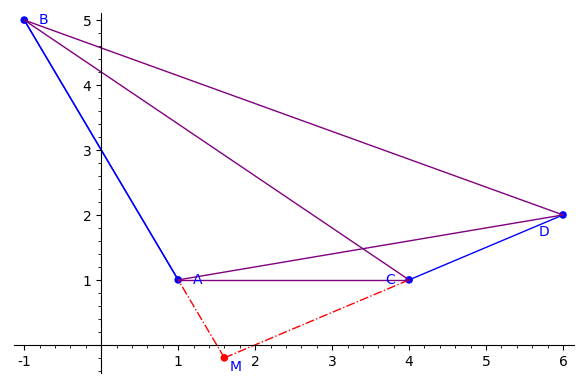
\includegraphics[width=\linewidth]{images/sageplot-2segments-perp.png}
\tcblower
\end{figureptx}%
\end{sbspanel}%
\begin{sbspanel}{0.5}%
\begin{figureptx}{Figure}{Two segments that are not perpendicular}{figure-fig-sageplot-2segments-notperp}{}%
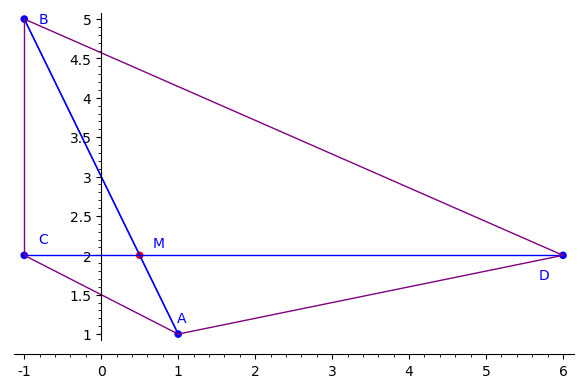
\includegraphics[width=\linewidth]{images/sageplot-2segments-notperp.png}
\tcblower
\end{figureptx}%
\end{sbspanel}%
\end{sidebyside}%
\end{proof}
\end{sectionptx}
%
%
\typeout{************************************************}
\typeout{Exercises 11.2 Exercises}
\typeout{************************************************}
%
\begin{exercises-section}{Exercises}{Exercises}{}{Exercises}{}{}{exercises-c-geometry-d}
\begin{divisionexercise}{1}{}{}{exercise-c-geometry-d-b}%
Prove that a central angle subtended by a given circular arc is twice the angle of an inscribed angle for the same arc.%
\end{divisionexercise}%
\begin{divisionexercise}{2}{}{}{exercise-c-geometry-d-c}%
Inscribe a rectangle of base \(b\) and height \(h\) and an isosceles triangle of base \(b\) in a circle of radius one as shown in \hyperref[figure-fig-geometry2]{Figure~{\xreffont\ref{figure-fig-geometry2}}}. For what value of \(h\) do the rectangle and triangle have the same area?%
\begin{figureptx}{Figure}{When do the rectangle and triangle have the same area?}{figure-fig-geometry2}{}%
\begin{image}{0.2}{0.6}{0.2}%
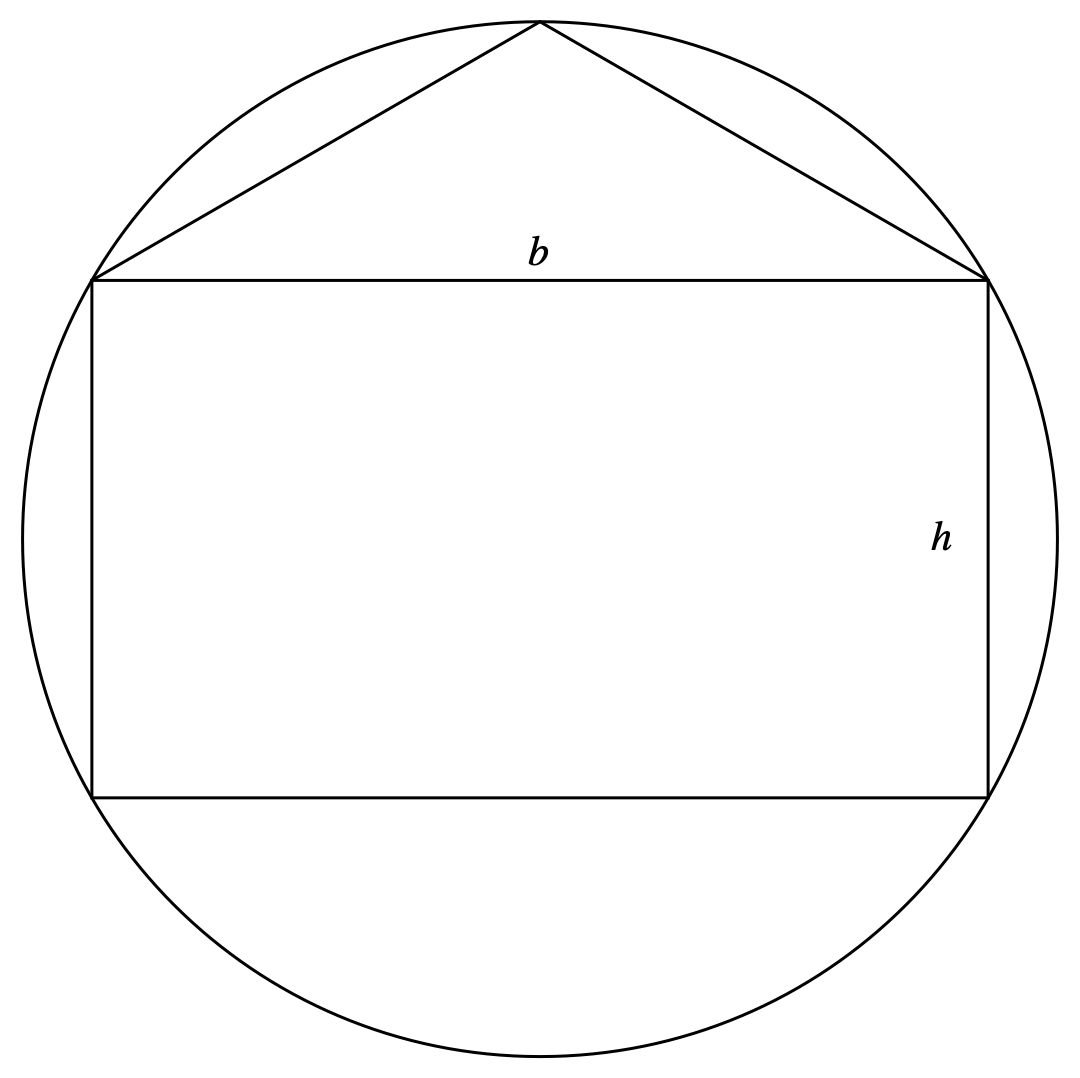
\includegraphics[width=\linewidth]{images/fig-geometry2.png}
\end{image}%
\tcblower
\end{figureptx}%
\end{divisionexercise}%
\begin{divisionexercise}{3}{}{}{exercise-c-geometry-d-d}%
What convex quadrilaterals can be inscribed into a circle? There is a name for these quadrilaterals, but your answer should describe them, not just name them%
\end{divisionexercise}%
\begin{divisionexercise}{4}{}{}{exercise-c-geometry-d-e}%
A rectangle with sides \(a\) and \(b\), \(a \lt b\) is rotated about its center, as shown in \hyperref[figure-rotated-rectangle]{Figure~{\xreffont\ref{figure-rotated-rectangle}}}, so that the two rectangles share two vertices. What is the area of the parallelogram that makes up the intersection of the two rectangles?%
\begin{figureptx}{Figure}{What is the area of the intersection?}{figure-rotated-rectangle}{}%
\begin{image}{0.2}{0.6}{0.2}%
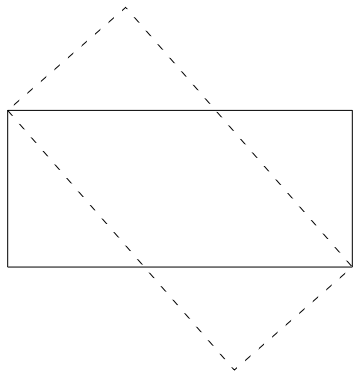
\includegraphics[width=\linewidth]{images/rotated-rectangle.png}
\end{image}%
\tcblower
\end{figureptx}%
\par\smallskip%
\noindent\textbf{\blocktitlefont Solution}.\hypertarget{solution-c-geometry-d-e-b}{}\quad{}Let \(c\) be the length of the horizontal sides of the parallelogram, so the area we are looking for is \(a c\). The triangles that are outside the parallelogram are right triangles with hypotenuse \(c\), and sides \(b-c\) and \(a\).%
\begin{equation*}
(b-c)^2+a^2= c^2 \Rightarrow \textrm{   }c=\frac{a^2+ b^2}{2b }\textrm{  }\Rightarrow \textrm{  Area } =\frac{a}{2b} \left(a^2+ b^2\right)
\end{equation*}
%
\end{divisionexercise}%
\begin{divisionexercise}{5}{}{}{exercise-c-geometry-d-f}%
Prove that if the lengths of the sides of a triangle form an arithmetic progression, then the radius of the inscribed circle is one third of one of the heights of the triangle.%
\par\smallskip%
\noindent\textbf{\blocktitlefont Hint}.\hypertarget{hint-c-geometry-d-f-b}{}\quad{}Try two-way counting.%
\par\smallskip%
\noindent\textbf{\blocktitlefont Solution}.\hypertarget{solution-c-geometry-d-f-c}{}\quad{}Assume the sides of the triangle are \(b-d\), \(b\), and \(b+d\); and that the altitude to the side of length \(b\) is \(h\). Let \(r\) be the radius of the inscribed circle.  If we connect the center of the inscribed circle to the vertices of the triangle, the area of the triangle is the sum of areas of three triangles with height \(r\) the sides of the triangles as bases.  Therefore,%
\begin{equation*}
\frac{1}{2} b \cdot h = \frac{1}{2} r(b-d)+ \frac{1}{2} r\cdot b+ \frac{1}{2} r(b+d) = \frac{1}{2}r(3\cdot b) = \frac{1}{2}b(3\cdot r)
\end{equation*}
Therefore, \(r=\frac{1}{3}\cdot h\)%
\end{divisionexercise}%
\begin{divisionexercise}{6}{}{}{exercise-c-geometry-d-g}%
A piece of paper is in the shape of a rectangle \(ABCD\) with \(AB=CD=3\) and \(AD=BC=5\). The paper is folded so that \(A\) and \(C\) coincide. Find the length of the crease.  Generalize your result.%
\par\smallskip%
\noindent\textbf{\blocktitlefont Hint}.\hypertarget{hint-c-geometry-d-g-b}{}\quad{}The line connecting \(A\) and \(C\) is perpendicular to the fold.%
\end{divisionexercise}%
\begin{divisionexercise}{7}{}{}{exercise-c-geometry-d-h}%
On the hyperbola \(x y = 1\) consider four points whose \(x\)-coordinates are \(x_1\), \(x_2\), \(x_3\), and \(x_4\). Show that if these points lie on a circle, then \(x_1 \cdot  x_{2} \cdot x_{3}\cdot x_4 = 1\).%
\par\smallskip%
\noindent\textbf{\blocktitlefont Solution}.\hypertarget{solution-c-geometry-d-h-b}{}\quad{}In order for a point \((x,y) =(x,\frac{1}{x})\) to be on the circle of radius \(c\) centered at \((a,b)\), it must be a root of the polynomial%
\begin{equation*}
x^4-2 a x^3 + (a^2+b^2-c^2)x^2 -2b x +1.
\end{equation*}
According to the Vieta relation for the constant term, the product of the four roots must equal 1.%
\end{divisionexercise}%
\begin{divisionexercise}{8}{}{}{exercise-c-geometry-d-i}%
Let \(ABC\) be a triangle and let the angle bisector of \(\angle A\) intersect the side \(BC\) at a point \(D\). Show that \(\frac{A B}{A C} = \frac{B D}{C D}\).%
\par\smallskip%
\noindent\textbf{\blocktitlefont Hint}.\hypertarget{hint-c-geometry-d-i-b}{}\quad{}Try the law of sines.%
\end{divisionexercise}%
\begin{divisionexercise}{9}{}{}{exercise-c-geometry-d-j}%
A trapezoid and a triangle are inscribed a circle. One side of the trapezoid is a diameter of the circle and the sides of the  triangle are parallel to sides of the trapezoid, as shown in \hyperref[figure-fig_trap_tri]{Figure~{\xreffont\ref{figure-fig_trap_tri}}}. Prove that the trapezoid and triangle have the same area.%
\begin{figureptx}{Figure}{Do the trapezoid and triangle have equal areas?}{figure-fig_trap_tri}{}%
\begin{image}{0.2}{0.6}{0.2}%
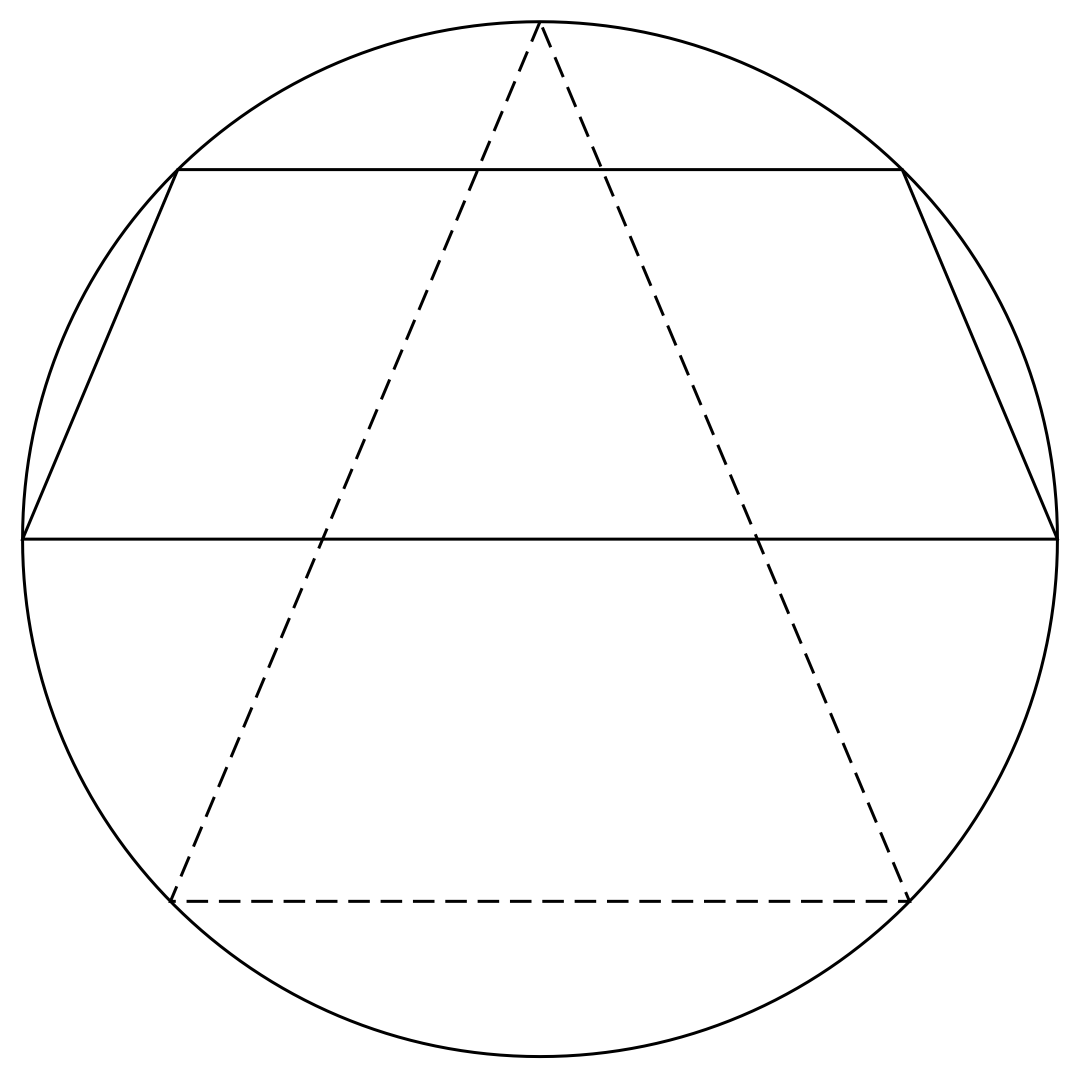
\includegraphics[width=\linewidth]{images/fig_trap_tri.png}
\end{image}%
\tcblower
\end{figureptx}%
\par\smallskip%
\noindent\textbf{\blocktitlefont Hint}.\hypertarget{hint-c-geometry-d-j-b}{}\quad{}Use coordinates with the circle at the origin and the diameter on the \(x\)-axis.  You can assume that the radius of the circle is \(1\).%
\end{divisionexercise}%
\begin{divisionexercise}{10}{}{}{exercise-c-geometry-d-k}%
Let \(f\) be a real-valued function on the plane such that for every square \(ABCD\) in the plane, \(f(A) + f(B) + f(C) + f(D) = 0\). Does it follow that \(f(P) = 0\) for all points \(P\) in the plane?%
\par\smallskip%
\noindent\textbf{\blocktitlefont Hint}.\hypertarget{hint-c-geometry-d-k-b}{}\quad{}Start with a square and divide it into four squares.%
\end{divisionexercise}%
\begin{divisionexercise}{11}{}{}{exercise-c-geometry-d-l}%
Given nine lattice points in \(\mathbb{R}^3\) prove that there exist two of them with the property that the midpoint of the segment between them is a lattice point.%
\end{divisionexercise}%
\begin{divisionexercise}{12}{}{}{exercise-c-geometry-d-m}%
Consider triangle \(ABC\) with the following trisection points,%
\begin{itemize}[label=\textbullet]
\item{}\(P\) on segment \(AB\) closest to \(B\)%
\item{}\(R\) on segment \(BC\) closest to \(C\) and%
\item{}\(Q\) on segment \(CA\) closest to \(A\).%
\end{itemize}
If these points are connected by segments to the opposite vertices of the triangle, is the area of the inner triangle created by the segments related to the area of triangle \(ABC\)?%
\end{divisionexercise}%
\end{exercises-section}
\end{chapterptx}
%
%
\typeout{************************************************}
\typeout{Chapter 12 Probability}
\typeout{************************************************}
%
\begin{chapterptx}{Chapter}{Probability}{}{Probability}{}{}{chapter-c-probability}
\renewcommand*{\chaptername}{Chapter}
\begin{introduction}{}%
If \(x\) is a random variable with outcomes \(x_1, x_2. x_3, \ldots\) and corresponding probabilities \(p_1, p_2, p_3, \ldots\), then the expected value of \(x\) is \(x_1p_2+ x_2p_2+ x_3p_3+\ldots\).%
\end{introduction}%
%
%
\typeout{************************************************}
\typeout{Section 12.1 Conditional Probability}
\typeout{************************************************}
%
\begin{sectionptx}{Section}{Conditional Probability}{}{Conditional Probability}{}{}{section-s-conditional-probability}
\begin{example}{Example}{Family Matters.}{example-ex-family-matters}%
Assume that the probability that a child is born a boy is exactly \(\frac{1}{2}\).  Now suppose you are told that a certain family has two children and one of them is a boy.  What is probability that the family has two boys?  Our intuition may tell us a certain answer, but many of us are wrong. This is a case for conditional probability.%
\end{example}
\begin{definition}{Definition}{Conditional Probability.}{definition-def-conditional-probability}%
\index{Conditional Probability}%
\label{notation-def-conditional-probability-c}%
Suppose a random event takes place and let \(H\) a condition on the event that has a positive probability. The probability that a second condition, \(A\), is met with knowledge that \(H\) is true is called the ``the probability of \(A\) conditioned on \(H\),'' denoted \(P(A \mid H)\).%
\end{definition}
\begin{theorem}{Theorem}{The Law of Conditional Probability.}{}{theorem-s-conditional-probability-d}%
Given a random event with a condition, \(H\), that has a positive probability. Let \(A\) be a second condition on this event.  Then%
\begin{equation*}
P(A \mid H)= \frac{P(A \wedge H)}{P(H)}
\end{equation*}
%
\end{theorem}
In the example above, the random event of two children being born in sequence has four equally likely outcomes; BB, BG, GB, GG.  We are told that one of the first three has occured, so \(P(H) =\frac{3}{4}\) in this case.   The condition that one of the children is boy and both are boys is the same the condition that both are boys, so \(P(A \wedge H) = \frac{1}{4}\) in this case, therefore the probability we want is \(\frac{1/4}{3/4} =\frac{1}{3}\).  This conclusion often surprises people.  Did it surprise you?%
\end{sectionptx}
%
%
\typeout{************************************************}
\typeout{Section 12.2 Geometric Probability}
\typeout{************************************************}
%
\begin{sectionptx}{Section}{Geometric Probability}{}{Geometric Probability}{}{}{section-s-geometric-probability}
Some probability problems can be solved using geometric means. Here is an example that illustrates the technique.%
\begin{example}{Example}{Throwing Darts.}{example-ex-geometric-probability}%
What is the probability that the sum of two randomly chosen numbers in the interval \([0, 1]\) does not exceed 1 and their product exceeds \(\frac{3}{16}\)?%
\par
This is a routine in that we can think of a selection of the random numbers as throwing a dart at a square dartboard so that each point on the dartboard is equally likely.  This isn't realistic for good dart players, but imagine it anyways!  The condition on which  we want to assess the probablity determines a region on the dartboard.  The area of that region divided by the total area of the dartboard, which is 1, is the probabily we are looking for.   This means the problem reduces to the computation of the area shown in \hyperref[figure-fig-geom-prob]{Figure~{\xreffont\ref{figure-fig-geom-prob}}}, which can be done with basic calculus in this case.%
\begin{figureptx}{Figure}{A target on a square dart board}{figure-fig-geom-prob}{}%
\begin{image}{0.2}{0.6}{0.2}%
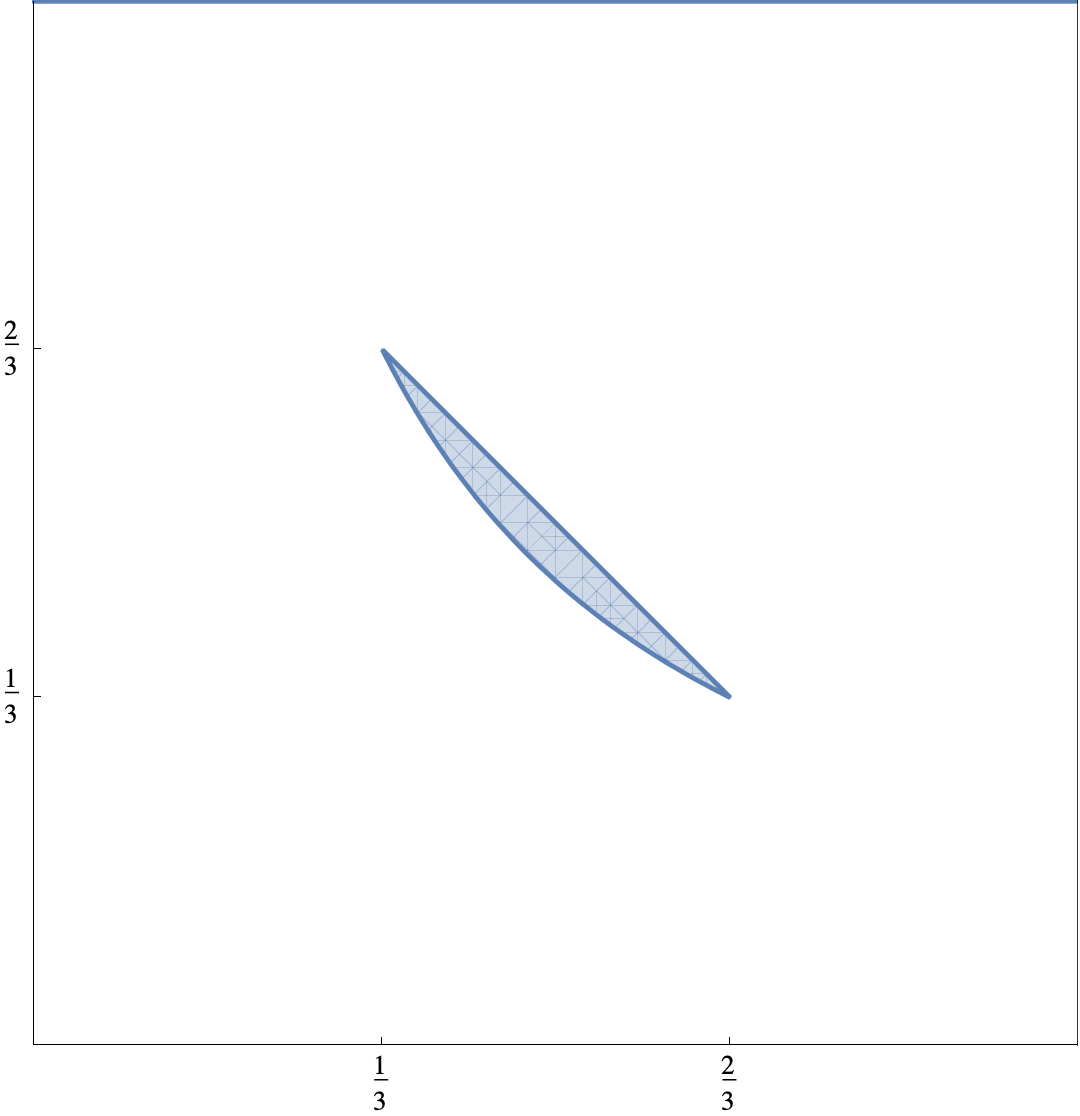
\includegraphics[width=\linewidth]{images/fig-geom-prob.png}
\end{image}%
\tcblower
\end{figureptx}%
\end{example}
The challenge of geometric probability problems tends to be identification of regions that represent the possible outcomes and the outcomes that are of interest. The dimension can be higher than two.%
\end{sectionptx}
%
%
\typeout{************************************************}
\typeout{Exercises 12.3 Exercises}
\typeout{************************************************}
%
\begin{exercises-section}{Exercises}{Exercises}{}{Exercises}{}{}{exercises-c-probability-e}
\begin{divisionexercise}{1}{}{}{exercise-c-probability-e-b}%
Suppose that \(n\)  integers, \(n \geq 3\) are randomly arranged in some list.  We might question whether they have ended up on strictly increasing order.   To test for this unlikely event, we might examine the first two numbers in the list.  Since their positions are random, the probability that they are in increasing order, is \(\frac{1}{2}\). If they are in order, we might next make a comparison of the second and third numbers, the third and fourth numbers, etc. Since each pair can be in it's current relative position or in the reverse, the probability of each pair being in order is \(\frac{1}{2}\). If we continue to the end with increasing orders and the last two integers are in order, then we might conclude that the probability that the whole list is ordered is \(\frac{1}{2^{n-1}}\).  Is this correct?%
\par\smallskip%
\noindent\textbf{\blocktitlefont Hint}.\hypertarget{hint-c-probability-e-b-b}{}\quad{}We wouldn't ask if the logic were correct!%
\par\smallskip%
\noindent\textbf{\blocktitlefont Solution}.\hypertarget{solution-c-probability-e-b-c}{}\quad{}This logic is incorrect.  Taken from a different point of view, there are \(n!\) ways in which the integers can be arranged, and only one of them is completely sorted, so the probability we seek is \(\frac{1}{n!}\).  How the logic that produces an incorrect result breaks down can be seen in the second step.  The first three numbers need to be in order.  It's true that the second and third numbers are in order is \(\frac{1}{2}\), but the probabilty that they are in order given that the first two are in order is \(\frac{1}{3}\).%
\begin{equation*}
P((k_2\lt k3)  \mid (k_1\lt k_2))= \frac{P((k_2\lt k_3) \land (k_1\lt k_2))}{P(k_1\lt k_2)}=\frac{1/6}{1/2}= \frac{1}{3}.
\end{equation*}
%
\end{divisionexercise}%
\begin{divisionexercise}{2}{}{}{exercise-c-probability-e-c}%
Steph Kuri shoots free throws on a basketball court. She makes the first and misses the second, and thereafter the probability that she makes the next shot is equal to the proportion of shots she has made so far. What is the probability that she makes exactly 50 of her first 100 shots?%
\end{divisionexercise}%
\begin{divisionexercise}{3}{}{}{exercise-c-probability-e-d}%
King Arthur is sick of fights for inheritance and decides to announce the following law. From now on, no family will be allowed to have another child after a boy is born. What will happen to the percentage of males if the law is followed?%
\end{divisionexercise}%
\begin{divisionexercise}{4}{}{}{exercise-c-probability-e-e}%
Four players in a game, N(orth), W(est), S(outh), and E(ast) sit at a round table. N holds a gold coin. One of three things happen, each with probability 1\slash{}3: N passes the coin to his right to W, N passes the coin to his left to E, or N walks away with the coin and the game is over. In the first two cases, the holder of the coin repeats the previous step, passing the coin to the right or left, or keeping the coin. What are the probabilities of winning for the four players?%
\par\smallskip%
\noindent\textbf{\blocktitlefont Solution}.\hypertarget{solution-c-probability-e-e-b}{}\quad{}We will abbreviate the probability that player \(X\) wins to \(P(X)\).  By the symmetry of the game, \(P(W)=P(E)\).  Also, we observe that%
\begin{equation*}
\begin{split}
P(W)&=P(W | \text{ the coin passes to }W)/3 + P(W |\text{ the coin passes to }E)/3\\
&=P(N)/3 + P(S)/3\\
\end{split}
\end{equation*}
and%
\begin{equation*}
\begin{split}
P(S)&=P(S | \text{ the coin passes to }W)/3 + P(S |\text{ the coin passes to }E)/3\\
&=P(W)/3 + P(E)/3 = \frac{2}{3} P(W)\\
\end{split}
\end{equation*}
Finally, since someone must win eventually, \(P(N)+P(W)+P(S)+P(E)=1\).  The four equations we have listed have the single solution \(P(N)=\frac{7}{15}\), \(P(W)=P(E)=\frac{1}{5}\), and \(P(S)=\frac{2}{15}\)%
\par
There are two other ways to reach the same solution to this problem.  One is to use the fact this is Markov Chain.  The game has eight states, four are for the situations where the coin has still not been won but is held one of the players.  The other four states are called absorbing states and represent the outcomes where each player can win.  In this context, we want to compute the probabilities of landing each of the absorbing states.  There are matrix techniques for computing these probabilities.  See Kemeny and Snell \hyperlink{biblio-biblio-kemeny}{[{\xreffont 12}]} for details. Another approach is to model the game with a \terminology{stochastic abacus}.  We recommend the reader to Propp \hyperlink{biblio-biblio-propp}{[{\xreffont 14}]} or Torrence \hyperlink{biblio-biblio-torrence}{[{\xreffont 16}]}  for information on this approach.%
\end{divisionexercise}%
\begin{divisionexercise}{5}{}{}{exercise-c-probability-e-f}%
Suppose two teams play a series of games in which the probability that either wins any of the games is \(\frac{1}{2}\).  If they play a best of seven series, where the winner is the first to win four games, what is the probability that the series lasts seven games?%
\par\smallskip%
\noindent\textbf{\blocktitlefont Answer}.\hypertarget{answer-c-probability-e-f-b}{}\quad{}\(\frac{5}{16}\)%
\par\smallskip%
\noindent\textbf{\blocktitlefont Solution}.\hypertarget{solution-c-probability-e-f-c}{}\quad{}In order for the series to go seven games, the teams must split the first six games. Imagine that they play out six games no matter what happens.  There are \(2^6\) equally likely outcomes and in \(\binom{6}{3}=20\) of the cases the teams split. Therefore, the probability of a seven games series \(\frac{20}{2^6}= \frac{5}{16}\).%
\end{divisionexercise}%
\begin{divisionexercise}{6}{Simplified NCAA basketball pool.}{}{exercise-c-probability-e-g}%
There are 64 teams who play single elimination tournament, hence 6 rounds, and you have to predict all the winners in all 63 games. Your score is then computed as follows: 32 points for correctly predicting the final winner, 16 points for each correct finalist, and so on, down to 1 point for every correctly predicted winner for the first round. Knowing nothing about any team, you flip fair coins to decide every one of your 63 bets. Compute your expected number of points.%
\end{divisionexercise}%
\begin{divisionexercise}{7}{}{}{exercise-c-probability-e-h}%
Three real numbers \(a\), \(b\), \(c\) are randomly (and uniformly) chosen from the interval \([0, 1]\). What is the probability that there exists a triangle with sides \(a\), \(b\), \(c\)?%
\par\smallskip%
\noindent\textbf{\blocktitlefont Solution}.\hypertarget{solution-c-probability-e-h-b}{}\quad{}Given any \(c\) between 0 and 1, we can determine the probablity that \(a\) and \(b\) combine with \(c\) to form a triangle by measuring the area of the region indicated by the inequalities in \hyperref[figure-fig-prob-of-triangle]{Figure~{\xreffont\ref{figure-fig-prob-of-triangle}}}. That probability is \(\frac{(4-3c)c}{2}\). We can then integrate this probability over the interval \([0,1]\) to get a probability for the three random numbers of \(\frac{1}{2}\)%
\begin{figureptx}{Figure}{Region of triangle formation}{figure-fig-prob-of-triangle}{}%
\begin{image}{0}{1}{0}%
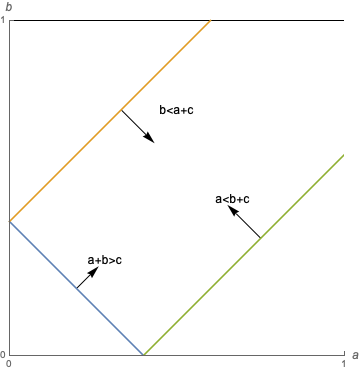
\includegraphics[width=\linewidth]{images/prob-of-triangle.png}
\end{image}%
\tcblower
\end{figureptx}%
\end{divisionexercise}%
\begin{divisionexercise}{8}{}{}{exercise-c-probability-e-i}%
Let \(p_n\) be the probability that \(c + d\) is a perfect square, where the integers \(c\) and \(d\) are selected independently at random from the set \(\{1, . . . , n\}\). Find \(\lim_{n\to \infty } \, \sqrt{n} p_n\).%
\par\smallskip%
\noindent\textbf{\blocktitlefont Hint}.\hypertarget{hint-c-probability-e-i-b}{}\quad{}Start by counting points in the diagonals of the square array of lattice points \((c,d)\) such that \(c+d\) is a square.  There are two formulae for the number of points: one for diagonals that produce the squares of the numbers 2 through \(\lfloor \sqrt{n+1} \rfloor\), and a second for those that produce squares of the the numbers from \(\lfloor \sqrt{n+1} \rfloor +1\) to \(\lfloor \sqrt{2n} \rfloor\).%
\end{divisionexercise}%
\begin{divisionexercise}{9}{}{}{exercise-c-probability-e-j}%
Two real numbers \(x\) and \(y\) are chosen at random in the interval \((0,1)\) with respect to the uniform distribution. What is the probability that the closest integer to \(x/y\) is even? Express the answer in the form \(r + s \pi\), where \(r\) and \(s\) are rational numbers.%
\end{divisionexercise}%
\begin{divisionexercise}{10}{}{}{exercise-c-probability-e-k}%
Let \(\alpha  \in  [0,1]\) be an arbitrary number, rational or irrational. The only randomizing device is an unfair coin, with probability \(p \in (0,1)\) of heads. Design a game between Alice and Bob so that Alice's winning probability is exactly \(\alpha\). The game has to end in a finite number of tosses with probability 1.%
\end{divisionexercise}%
\begin{divisionexercise}{11}{}{}{exercise-c-probability-e-l}%
Begin with the set \(\{1,2,\dots,n\}\). Toss a coin \(n\) times, once for each member of the set. Keep the elements that scored ``Heads'' and discard the elements that got ``Tails''. You now have a certain subset \(S\) of the original set. Call this whole process a ``step''. Now take a step from \(S\). That is, toss a coin for each element of \(S\), and keep those that get ``Heads'', getting a sub-subset \(S'\), etc. This game halts when the empty set is reached. Let \(f(n,k,r)\) be the probability that after \(k\) steps, exactly \(r\) objects remain.%
\begin{enumerate}[label=(\alph*)]
\item{}Find a recurrence relation for \(f\), find the generating function for \(f\), and find \(f\) itself.%
\item{}What is the average number of steps in a complete game?%
\end{enumerate}
%
\end{divisionexercise}%
\begin{divisionexercise}{12}{}{}{exercise-c-probability-e-m}%
An urn contains a number of colored balls, with the same number of balls in each color. If 20 balls of a new color are added to the urn, the probability of drawing (without replacement) two balls of the same color is not changed. How many balls are in the urn (before the new balls are added)?%
\par\smallskip%
\noindent\textbf{\blocktitlefont Solution}.\hypertarget{solution-c-probability-e-m-b}{}\quad{}Let \(c\) be the number of colors represented in the urn and \(n\) the number of balls of each color.  The condition we want to satisfy is \(\frac{c (n-1) n+380}{(c n+19)
(c n+20)}=\frac{n-1}{c n-1}\).  Manipulating this equation, we get \(\frac{n (c (2 n-21)+19)}{(c
n-1) (c n+19) (c n+20)}=0\), which implies that \(c(2 n-21)+19=0\).  The only pair integer pairs \((c,n)\) to this equation are \((1,1)\) and \((19,10)\).  The first must be rejected, and so the only solution is that there are initially 10 balls of each of 19 colors. Adding 20 of a new color will not change the probability of matching colors.  In either case the probability will be \(\frac{1}{21}\). This is the only solution.%
\end{divisionexercise}%
\begin{divisionexercise}{13}{}{}{exercise-c-probability-e-n}%
Suppose that the probability that the length of a telephone call is between \(t_1\) and \(t_2\) minutes,  \(t_1 \lt t_2\) is \(\int_{t_1}^{t_2} e^{-t} \, dt\).   What is the probability that a phone call lasts less than one minute.  What is the probability that a phone call lasts less than two minutes given that it lasts at least one minute?%
\par\smallskip%
\noindent\textbf{\blocktitlefont Solution}.\hypertarget{solution-c-probability-e-n-b}{}\quad{}Let \(X\) be a random variable that is the length of a phone call. The probability that a call lasts no more than one minute is \(Pr(X \lt 1) = \int_{0}^{1} \, e^{-t} dt = \frac{e-1}{e}\).  The probability that it lasts less than two minutes given that it last at least one minute is%
\begin{equation*}
Pr(X \lt 2 | X \geq 1)= \frac{Pr(1 \leq X \lt 2)}{Pr(X \geq 1)} = \frac{\frac{e-1}{e^2}}{\frac{1}{e}}=\frac{e-1}{e}
\end{equation*}
The property that these two probabilities are equal is called  memorylessness.%
\end{divisionexercise}%
\end{exercises-section}
\end{chapterptx}
%
%
\typeout{************************************************}
\typeout{Chapter 13 Linear Algebra}
\typeout{************************************************}
%
\begin{chapterptx}{Chapter}{Linear Algebra}{}{Linear Algebra}{}{}{chapter-c-linear-algebra}
\renewcommand*{\chaptername}{Chapter}
%
%
\typeout{************************************************}
\typeout{Section 13.1 Examples}
\typeout{************************************************}
%
\begin{sectionptx}{Section}{Examples}{}{Examples}{}{}{section-sect-linear-examples}
\begin{example}{Example}{Oddtown.}{example-ex-oddtown-la}%
In a town with \(n\) people, \(m\) clubs have been formed. Every club has an odd number of members, and every two clubs have an even number of members in common. Prove that \(m \leq  n\).%
\par
Let \(v_i\) be the membership vector for club \(i\):  \((v_i)_j = 1\) if and only if person  \(j\) belongs to club \(i\). We view these \(m\) vectors as being in the vector space \(\mathbb{Z}_2^n\) of \(n\)-tuples of integers mod 2.  We will prove that the set of vectors \(\{v_1, v_2, \dots, v_m\}\) is linearly independent, which implies that \(m \leq  n\).%
\par
The conditions of problem translate to the following with respect to the dot products of these vectors.%
\begin{equation*}
\textrm{Each club has an odd number of members }\Rightarrow  v_i\cdot v_i = 1
\end{equation*}
and%
\begin{equation*}
\textrm{Any two clubs have an even number of members in common }\Rightarrow  v_i\cdot v_j = 0 \textrm{ if }i\neq j
\end{equation*}
%
\par
Now, assume  \(\sum_{i=1}^m c_i v_i = \vec{0}\).  We will show that each \(c_k = 0\) using the linearity of the dot product.%
\begin{equation*}
\begin{split}
0 & = v_k \cdot \vec{0}\\
& = v_k \cdot \sum_{i=1}^m c_i v_i\\
& = \sum_{i=1}^m c_i (v_k \cdot v_i)\\
& = c_k (v_k \cdot v_k)\\
& = c_k
\end{split}
\end{equation*}
Therefore we have derived the inequality.%
\end{example}
\end{sectionptx}
%
%
\typeout{************************************************}
\typeout{Exercises 13.2 Exercises}
\typeout{************************************************}
%
\begin{exercises-section}{Exercises}{Exercises}{}{Exercises}{}{}{exercises-c-linear-algebra-c}
\begin{divisionexercise}{1}{}{}{exercise-c-linear-algebra-c-b}%
Let \(N=2^n\) for some positive integer \(n\) and \(\omega =e^{\frac{2\pi i}{N}}\).  Let \(U(\omega )\) be the \(N\times N\) matrix with \(U(\omega)_{i,j}= \omega^{(i-1)(j-1)}\).  Compute \(U(\omega )U\left(\omega ^{-1}\right)\).%
\end{divisionexercise}%
\begin{divisionexercise}{2}{}{}{exercise-c-linear-algebra-c-c}%
Let \(A\) and \(B\) be \(n\times n\) matrices satisfying \(A+B = A B\). Show that \(A B = B A\).%
\par\smallskip%
\noindent\textbf{\blocktitlefont Solution}.\hypertarget{solution-c-linear-algebra-c-c-b}{}\quad{}Consider the product \((I-A)(I-B)\).%
\end{divisionexercise}%
\begin{divisionexercise}{3}{}{}{exercise-c-linear-algebra-c-d}%
Consider the matrix equation \(\left(
\begin{array}{ccc}
1 & 1 & 0 \\
1 & 1 & 1 \\
0 & 1 & 1 \\
\end{array}
\right)^n=\left(
\begin{array}{ccc}
A_n & B_n & C_n \\
D_n & E_n & F_n \\
G_n & H_n & J_n \\
\end{array}
\right)\).  Identify formulae for \(A_n, B_n,\ldots , J_n\).%
\end{divisionexercise}%
\begin{divisionexercise}{4}{}{}{exercise-c-linear-algebra-c-e}%
Let \(A\) be a square matrix, \(A \neq I\), and suppose there exists a positive integer \(m\) such that \(A^m=I\).  Calculate \(det(I + A + A^2 + \cdots + A^{m-1})\).%
\par\smallskip%
\noindent\textbf{\blocktitlefont Hint}.\hypertarget{hint-c-linear-algebra-c-e-b}{}\quad{}The matrix that you want the determinant of is a finite geometric series.%
\par\smallskip%
\noindent\textbf{\blocktitlefont Solution}.\hypertarget{solution-c-linear-algebra-c-e-c}{}\quad{}In general, we have%
\begin{equation*}
(I +  A + A^2 + \cdots + A^{m-1})(I -A)=(I-A^m).
\end{equation*}
But the right side is the zero matrix and so for every nonzero vector \(x\),%
\begin{equation*}
(I +  A + A^2 + \cdots + A^{m-1})(I -A)\vec{x}=\vec{0}.
\end{equation*}
Since \(I-A \neq \vec{O}\), there exist nonzero vectors \(\vec{x}\) and \(\vec{y}\) such that \((I-A)\vec{x} = \vec{y}\).  This gives us%
\begin{equation*}
(I +  A + A^2 + \cdots + A^{m-1})\vec{y}=\vec{0}
\end{equation*}
which implies that \(I +  A + A^2 + \cdots + A^{m-1}\) is singular and so its determinant is zero.%
\par
This problem was from the 2006 MAA Northeast Section Math Competition.%
\end{divisionexercise}%
\begin{divisionexercise}{5}{}{}{exercise-c-linear-algebra-c-f}%
Let's call a real \(3 \times 3\) matrix a ``magic square'' if all its row-sums and column-sums are equal to 0. Show that all magic squares form a vector space. Find its dimension.%
\par\smallskip%
\noindent\textbf{\blocktitlefont Solution}.\hypertarget{solution-c-linear-algebra-c-f-b}{}\quad{}The dimension is four.  If we let the entries in the two by two block in the top left of the a matrix be arbitrary, then the other five entries are determined in the pattern%
\begin{equation*}
\left(
\begin{array}{ccc}
x_1 & x_2 & -x_1-x_2 \\
x_3 & x_4 & -x_3-x_4 \\
-x_1-x_3 & -x_2-x_4 & x_1+x_2+x_3+x_4 \\
\end{array}
\right)
\end{equation*}
This produces a set of four matrices that can easily be shown to be linearly independent and so is a basis.%
\end{divisionexercise}%
\begin{divisionexercise}{6}{}{}{exercise-c-linear-algebra-c-g}%
Let \(n\) be a positive integer, and let \(v_1, v_2, \ldots ,v_k\), \(1\leq k\leq n\), be linearly independent vectors in \(\mathbb{R}^n\) spanning a subspace \(V_k\). Prove that there exist \(k\) orthogonal vectors \(w_1, w_2, \ldots ,w_k\) that span \(V_k\).  (Note: Two nonzero vectors are orthogonal if their dot product is equal to 0.)%
\par\smallskip%
\noindent\textbf{\blocktitlefont Hint}.\hypertarget{hint-c-linear-algebra-c-g-b}{}\quad{}Use the linearly of the dot product: \(x.(a y+z) = a(x.y)+x.z\), where \(a\) is a scalar.%
\end{divisionexercise}%
\begin{divisionexercise}{7}{}{}{exercise-c-linear-algebra-c-h}%
Let \(A\) be the \(n\times n\) matrix whose entry in the \(i\)-th row and \(j\)-th column is \(\frac{1}{\min (i,j)}\) for \(1 \leq  i,j \leq  n\). Compute \(\det (A)\).%
\par\smallskip%
\noindent\textbf{\blocktitlefont Hint}.\hypertarget{hint-c-linear-algebra-c-h-b}{}\quad{}Expand the determinant along the last row of the matrix.%
\par\smallskip%
\noindent\textbf{\blocktitlefont Solution}.\hypertarget{solution-c-linear-algebra-c-h-c}{}\quad{}Let \(A_n\) be the \(n\) by \(n\) version of the matrix. Assume \(n \geq 3\). Expand the determinant of \(A_n\) along the last row. If \(1 \leq k \leq n-1\) then the minor \(M_{n k}\) is the determinant of a matrix with two identical columns, which is zero.    This leaves two nonzero term in the expansion. In both of the terms, the minor is the determinant of \(A_{n-1}\).  Therefore,%
\begin{equation*}
det(A_{n}) = - a_{n,n-1}  det(A_{n-1}) + a_{n,n-1}  det(A_{n-1}) =\frac{-1}{(n-1)n} \cdot det(A_{n-1}).
\end{equation*}
%
\par
Combining this recursion with the initial values of \(det(A_{1})=1\) and \(det(A_{2})=-\frac{1}{2}\), we see that  \(det(A_{n}) = \frac{(-1)^n}{n! (n-1)!}\)%
\end{divisionexercise}%
\begin{divisionexercise}{8}{}{}{exercise-c-linear-algebra-c-i}%
The dashboard of a nuclear power station has several lights. Some lights are on and some are off. There are also several buttons. Pressing each button changes the state of several lights (from on to off and from off to on). It is known that for every set of lights there exists a button connected to an odd number of lights in this set. Show that one can turn off all lights by pressing some buttons.%
\par\smallskip%
\noindent\textbf{\blocktitlefont Hint}.\hypertarget{hint-c-linear-algebra-c-i-b}{}\quad{}Start by creating a matrix, one row for each button and a column for each light.%
\par\smallskip%
\noindent\textbf{\blocktitlefont Solution}.\hypertarget{solution-c-linear-algebra-c-i-c}{}\quad{}Assume there are \(n\) buttons and \(m\) lights.  Let \(A\) be the \(n \times m\) matrix such that \(A_{i j} = 1\) if and only if button \(i\) is connected to light \(j\).  Let \(\Delta\) be a set of lights.  We represent this set by an \(m\) dimensional column vector \(\delta\) such that \(\delta_{i} = 1\) if and only if light \(i\) is in \(\Delta\).  The given condition on sets of lights implies that if \(\Delta\) is a nonzero vector, \(A \Delta\) is nonzero. Therefore, the columns of \(A\) are linearly independent, \(m \leq n\) and the rank of \(A\) is \(m\).  This implies that the column span of the transpose of \(A\) is full and every configuration of lights can be switched with some set of buttons.%
\end{divisionexercise}%
\begin{divisionexercise}{9}{}{}{exercise-c-linear-algebra-c-j}%
Compute the determinant of the \(n \times  n\) matrix \(\left[a_{i j}\right]\) such that \(a_{i j} =\lvert i-j\rvert\).%
\end{divisionexercise}%
\begin{divisionexercise}{10}{}{}{exercise-c-linear-algebra-c-k}%
Think of a square matrix as placed on a checkerboard, so that the leading diagonal consists entirely of white squares. Then if the signs of all the entries on black squares are changed, prove that the eigenvalues are unchanged.%
\par\smallskip%
\noindent\textbf{\blocktitlefont Solution}.\hypertarget{solution-c-linear-algebra-c-k-b}{}\quad{}Let \(M\) be the diagonal matrix with \(M_{i i}=(-1)^i\).  Then if \(A\) is the given square matrix, \(M A M\) is the matrix that has the ``black entries'' of \(A\) negated.%
\end{divisionexercise}%
\begin{divisionexercise}{11}{}{}{exercise-c-linear-algebra-c-l}%
It is well known that all real-valued functions on \(\mathbb{R}\) form a vector space. Does the function \(\sin  x\) belong to the linear span of the functions \(1\), \(\cos x\), \(\cos 2 x\), \(\cos 3 x,\ldots\)?    How about the function \(\sin^2 x\)?%
\par\smallskip%
\noindent\textbf{\blocktitlefont Solution}.\hypertarget{solution-c-linear-algebra-c-l-b}{}\quad{}Since \(\sin  x\) is an odd function and any linear combination of the cosines is even, so \(\sin  x\) is not in the linear span of cosines.  Using the double angle formula for cosine, we can derive \(\sin^2 x = \frac{1}{2}-\frac{1}{2} \cos (2 x)\), and so \(\sin^2 x\) is in the span of cosines.%
\par
Alternate solution: Suppose \(\sin x = \sum_{k=1}^m \lambda_k \cos{k x}\). Then we should have%
\begin{equation*}
\int_{-\pi }^{\pi } \sin^2(x) \, dx = \int_{-\pi }^{\pi } \sin(x)(\sum_{k=1}^m \lambda_k \cos{k x} ) \, dx
\end{equation*}
%
\end{divisionexercise}%
\end{exercises-section}
\end{chapterptx}
%
%
\typeout{************************************************}
\typeout{Chapter 14 Abstract Algebra}
\typeout{************************************************}
%
\begin{chapterptx}{Chapter}{Abstract Algebra}{}{Abstract Algebra}{}{}{chapter-c-abstract-algebra}
\renewcommand*{\chaptername}{Chapter}
\begin{introduction}{}%
Groups and finite fields are among the topics that have made their way into the Putnam lately.%
\end{introduction}%
%
%
\typeout{************************************************}
\typeout{Section 14.1 Groups}
\typeout{************************************************}
%
\begin{sectionptx}{Section}{Groups}{}{Groups}{}{}{section-c-abstract-algebra-c}
Let \(G\) be a group. Recall that the order of  \(g \in G\) is the minimum positive integer \(k\) such that \(g^k\) is the group identity.%
\begin{example}{Example}{1969 Putnam, altered.}{example-c-abstract-algebra-c-c}%
Show that a group cannot be the union of two of its proper subgroups.%
\par
Assume \(H\) and \(K\) are subgroups of some group \(G\), and that \(x \in H-K\), \(y \in K-H\).  We know that \(x*y\) must be in either \(H\) or \(K\).  Assume it's in \(H\).%
\begin{equation*}
x \in H \Rightarrow x^{-1} \in H \Rightarrow x^{-1}*(x*y) = y \in H
\end{equation*}
This contradiction implies that no such pair of subgroups exists.%
\end{example}
\end{sectionptx}
%
%
\typeout{************************************************}
\typeout{Section 14.2 Rings and Fields}
\typeout{************************************************}
%
\begin{sectionptx}{Section}{Rings and Fields}{}{Rings and Fields}{}{}{section-c-abstract-algebra-d}
Problem: Assume that \(p(x)\) is a polynomial of degree \(n\) over a field \(F\) that has \(n\) distinct roots in \(F\). Let \(I=(p(x)) = \{s(x)p(x) \mid s(x)\in F[x]\}\) be the principle ideal generated by \(p(x)\).  Characterize the factor ring \(F[x]/I\).%
\par
Assume%
\begin{equation*}
p(x)= \prod_{k=1}^n (x-\alpha_k),
\end{equation*}
where the \(\alpha_k\)'s are distinct elements of \(F\). We can show that \(F[x]/I\) is isomorphic to the ring \(F^n\) of \(n\)-tuples of elements of \(F\) with coordinatewise operations over \(F\).  Define \(\phi:F[x]/I \rightarrow F^n\) by%
\begin{equation*}
\phi(r(x)+I)=(r(\alpha_1),r(\alpha_2),\dots,r(\alpha_n))
\end{equation*}
%
\par
We leave it to the reader to verify that \(\phi\) is an isomorphism by checking the following:%
\begin{itemize}[label=\textbullet]
\item{}\(\phi\) is well defined bijection.%
\item{}For all \(r(x)+I, s(x)+I  \in F[x]/I\):%
\begin{equation*}
\phi((r(x)+I)+(s(x)+I))= \phi(r(x)+I)+\phi(s(x)+I)
\end{equation*}
%
\item{}For all \(r(x)+I, s(x)+I  \in F[x]/I\):%
\begin{equation*}
\phi((r(x)+I)\cdot (s(x)+I))= \phi(r(x)+I)\cdot \phi(s(x)+I)
\end{equation*}
%
\end{itemize}
A quick note on the need \(\phi\) to be well defined.  Since the same coset can be generated from different polynomials, and since \(\phi\) is defined in terms of a generating polynomial, we need to be sure that if \(s(x)\) and \(t(x)\) are different polynomials for which \(s(x)+I=t(x)+I\), we get \(\phi(s(x)+I)=\phi(t(x)+I)\).%
\end{sectionptx}
%
%
\typeout{************************************************}
\typeout{Exercises 14.3 Exercises}
\typeout{************************************************}
%
\begin{exercises-section}{Exercises}{Exercises}{}{Exercises}{}{}{exercises-c-abstract-algebra-e}
\begin{divisionexercise}{1}{}{}{exercise-c-abstract-algebra-e-b}%
Let \(S\) be a set which is closed under the binary operation \(\circ\), with the following properties:%
\begin{itemize}[label=\textbullet]
\item{}There is an element \(e \in S\) such that \(a \circ e = e\circ a=a, \forall a\in S\)%
\item{}\((a \circ b) \circ (c \circ d) = (a \circ c) \circ (b \circ d) \forall a,b,c,d \in  S\).%
\end{itemize}
%
\par
Prove or disprove:%
\begin{enumerate}[label=(\alph*)]
\item{}\(\circ\)  is associative on \(S\)%
\item{}\(\circ\)  is commutative on S%
\end{enumerate}
%
\end{divisionexercise}%
\begin{divisionexercise}{2}{}{}{exercise-c-abstract-algebra-e-c}%
Let \(*\) be an associative binary operation on a set \(A\) such that for all \(a, b \in A\), \(a*b=b*a \Rightarrow a=b\).  Prove that for all \(a, b, c \in A\), \(a*b*c = a*c\).%
\par\smallskip%
\noindent\textbf{\blocktitlefont Solution}.\hypertarget{solution-c-abstract-algebra-e-c-b}{}\quad{}Step 1: Note that the operation must be idempotent.  By associativity, \((a*a)*a = a*(a*a)\), and so \(a*a=a\).%
\par
Step 2: Show that for all \(a, b\), \(a*b*a=a\):%
\begin{equation*}
\begin{split}
(a*b*a)*a &= (a*b)*(a*a)\\
&=(a*b*a)\\
&=((a*a)*b*a)\\
&= a*(a*b*a) \Rightarrow a*b*a = a
\end{split}
\end{equation*}
%
\par
Step 3: Prove that \(a*b*c=a*c\).%
\begin{equation*}
(a*b*c)*(a*c)= (a*(b*c)*a)*c = a*c
\end{equation*}
while%
\begin{equation*}
(a*c)(a*b*c)= a*(c*(a*c)*c)= a*c
\end{equation*}
hence the conclusion.%
\end{divisionexercise}%
\begin{divisionexercise}{3}{}{}{exercise-c-abstract-algebra-e-d}%
(Putnam 1972) Let \(S\) be a set and \(\) a binary operation on \(S\) satisfying the laws%
\begin{enumerate}[label=(\roman*)]
\item{}\(x(xy)=y\) for all \(x,y \in S\)%
\item{}\((yx)x=y\) for all \(x,y \in S\)%
\end{enumerate}
Show that \(*\) is commutative but not necessarily associative.%
\par\smallskip%
\noindent\textbf{\blocktitlefont Solution}.\hypertarget{solution-c-abstract-algebra-e-d-b}{}\quad{}Step 1: Show that \(x*(y*x)=(x*y)*x = y\) for all \(x,y \in S\)%
\begin{equation*}
\begin{split}
y &=(y*(y*x))*(y*x)\\
&=x*(y*x)
\end{split}
\end{equation*}
and we can get \((x*y)*x\)	similarly.  Combining these equalities with the two given ones, we see that the product of three factors with one pair of equal ones can be commuted and associated in any order and the result is the unique factor.%
\par
Step 2: We can now get commutivity:%
\begin{equation*}
\begin{split}
y*x &= (x*(y*x))*x\\
&=x*((y*x)*x)\\
&=x*y
\end{split}
\end{equation*}
%
\par
We haven't used general associativity here, and in fact there are nonassociative binary operations that satisfy the premises. One such is the operation on the integers defined by \(x*y = -(x+y)\).%
\end{divisionexercise}%
\begin{divisionexercise}{4}{}{}{exercise-c-abstract-algebra-e-e}%
Let \(G\) be a finite group with identity \(e\).  If \(G\) contains distinct elements \(g\) and \(h\), neither equal to \(e\), such that%
\begin{equation*}
g^5=e \textrm{  and  }g h g^{-1} = h^2,
\end{equation*}
determine the order of \(h\).%
\par\smallskip%
\noindent\textbf{\blocktitlefont Solution}.\hypertarget{solution-c-abstract-algebra-e-e-b}{}\quad{}Start with \(g^2 h (g^{-1})^{2}\) and note that it reduces to \(h^4\).  Repeat with \(g^3\) replacing \(g^2\) and continue the pattern to conclude that \(h^{32}=h\).  This implies that \(h^{31}=e\) and since 31 is prime the order of \(h\) must be 31.%
\end{divisionexercise}%
\begin{divisionexercise}{5}{}{}{exercise-c-abstract-algebra-e-f}%
\index{Symmetric Group}%
In abstract algebra, the symmetric group \(S_n\) is the group of all permutations on \(\{1, 2, \dots, n\}\); i. e., bijections on \(\{1, 2, \dots, n\}\).  A transposition in \(S_n\) is a function \(\tau\) such that \(\tau(i)=j\) and \(\tau(j)=i\), where \(i \neq j\) and \(\tau(k)=k\) for \(k \neq i, j\).  A fundamental theorem involving permutations (which we will take as given) is that every permutation is a composition of an even number of transpositions or  an odd number of transpositions, but not both.   Prove that exactly half of the elements of \(S_n\) are ``even.''%
\end{divisionexercise}%
\begin{divisionexercise}{6}{}{}{exercise-c-abstract-algebra-e-g}%
\(S_n\) is a group of order \(n!\).  What is the smallest value of \(n\) for which there exists an element of order 10?, of order 20?%
\end{divisionexercise}%
\begin{divisionexercise}{7}{}{}{exercise-c-abstract-algebra-e-h}%
Consider the puzzle below, where one can rotate each of the three triangles. For example, rotating the middle triangle in (A) once gives the configuration in (B).%
\begin{figureptx}{Figure}{Spinning Triangles Puzzle}{figure-fig-group-puzzle-1}{}%
\begin{image}{0}{1}{0}%
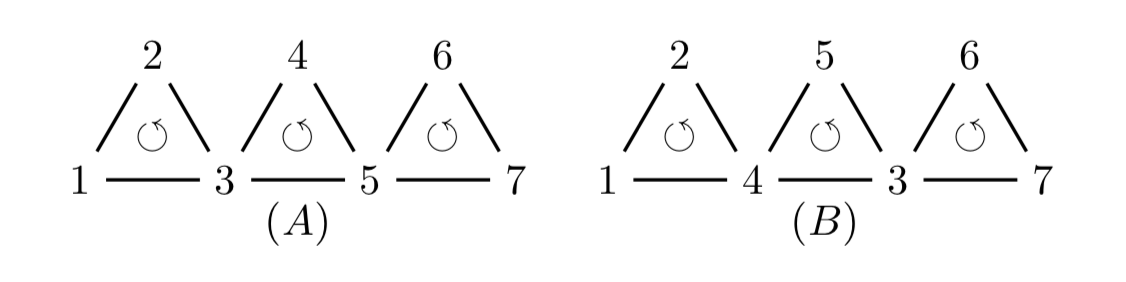
\includegraphics[width=\linewidth]{images/fig-group-puzzle-1.png}
\end{image}%
\tcblower
\end{figureptx}%
Prove that it there is no sequence of rotations that produce the following configuration, starting from (A).%
\begin{figureptx}{Figure}{Spinning Triangles Puzzle - Impossible Configuration}{figure-fig-group-puzzle-2}{}%
\begin{image}{0}{1}{0}%
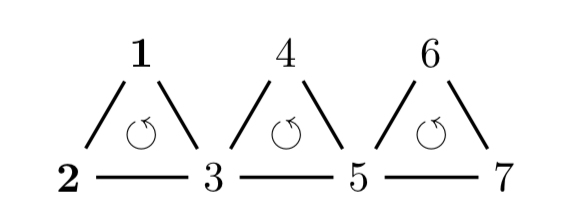
\includegraphics[width=\linewidth]{images/fig-group-puzzle-2.png}
\end{image}%
\tcblower
\end{figureptx}%
\par\smallskip%
\noindent\textbf{\blocktitlefont Solution}.\hypertarget{solution-c-abstract-algebra-e-h-b}{}\quad{}Every 120 degree spin of a triangle is an even permutation of the vertices. Therefore, any configuration that is reached starting at (A) must be even.  The configuration we are asked to consider is a single transposition of the vertices 1 and 2, which is an odd permutation.%
\end{divisionexercise}%
\end{exercises-section}
\end{chapterptx}
%
%
\typeout{************************************************}
\typeout{Chapter 15 2020 UML Problem Solving Competition}
\typeout{************************************************}
%
\begin{chapterptx}{Chapter}{2020 UML Problem Solving Competition}{}{2020 UML Problem Solving Competition}{}{}{chapter-c-competition_2020}
\renewcommand*{\chaptername}{Chapter}
\begin{introduction}{}%
A three hour local competition was held on December 5, 2020 in place of the Putnam, which was delayed until February 2021.%
\end{introduction}%
%
%
\typeout{************************************************}
\typeout{Section 15.1 Results}
\typeout{************************************************}
%
\begin{sectionptx}{Section}{Results}{}{Results}{}{}{section-c-competition_2020-c}
%
\begin{itemize}[label=\textbullet]
\item{}First Place:  Payton Collins, Senior Math major%
\item{}Second Place: Nurlan Gasimli, Freshman Math major%
\item{}Third Place: Charles Mirabile, Senior CS major%
\item{}Second Place among Freshmen\slash{}Sophomores:  Hunter Marion, Sophomore Math major%
\end{itemize}
%
\end{sectionptx}
%
%
\typeout{************************************************}
\typeout{Exercises 15.2 Problems}
\typeout{************************************************}
%
\begin{exercises-section}{Exercises}{Problems}{}{Problems}{}{}{exercises-c-competition_2020-d}
\begin{divisionexercise}{1}{}{}{exercise-c-competition_2020-d-b}%
Let \(R\) denote the set of points \((x, y)\) satisfying \(x^2 - 4 \lvert x \rvert +y^2 + 3 \leq 0\). What is the area of \(R\)?%
\par\smallskip%
\noindent\textbf{\blocktitlefont Answer}.\hypertarget{answer-c-competition_2020-d-b-b}{}\quad{}\(2\pi\).%
\par\smallskip%
\noindent\textbf{\blocktitlefont Solution}.\hypertarget{solution-c-competition_2020-d-b-c}{}\quad{}If \(x \geq 0\), then the inequality is \((x-2)^2 +y^2 \le 1\), which is a disk of radius \(1\) entirely to the right of the \(y\) axis, which has area \(\pi\).  If \(x \lt 0\), then the inequality is \((x+2)^2 +y^2 \le 1\) which is a disk of radius \(1\) entirely to the left of the \(y\) axis, which has area \(\pi\).%
\end{divisionexercise}%
\begin{divisionexercise}{2}{}{}{exercise-c-competition_2020-d-c}%
Let \(f(n)\) be the number of \(n\)-letter words that can formed with the letters A,B,C and such that the letter A occurs an even number of times. For example, when \(n = 1\), there are 2 such words, namely B,C so \(f (1) = 2\); when \(n = 2\), there are 5 such words, namely AA,BB,BC,CB,CC, so \(f(2) = 5\). Find, with proof, a simple formula for \(f(n)\). (The formula should not involve a summation.)%
\par\smallskip%
\noindent\textbf{\blocktitlefont Answer}.\hypertarget{answer-c-competition_2020-d-c-b}{}\quad{}\(f(n)= \frac{1}{2} \left(1+3^n\right)\)%
\par\smallskip%
\noindent\textbf{\blocktitlefont Solution}.\hypertarget{solution-c-competition_2020-d-c-c}{}\quad{}One solution to this problem is to identify that if a string of length \(n\), \(n \geq 2\), is to be counted, then either it ends in a A or it doesn't. If it ends in an A, then it is preceeded by a string of length \(n-1\) that isn't counted because there are an odd number of A's in that string.   If the string does not end with an A, then it is proceeded by a one of the \(f(n-1)\) strings that we are counting.  Therefore, \(f(n)\) satisfies the equations%
\begin{equation*}
f(n)= (3^{n-1} -f(n-1))+ 2\,f(n-1) \textrm{   and    } f(1)=2\text{.}
\end{equation*}
%
\end{divisionexercise}%
\begin{divisionexercise}{3}{}{}{exercise-c-competition_2020-d-d}%
An equilateral triangle in the first quadrant has vertices at the points \((0, 0)\), \((x_1, 5)\), and \((x_2, 12)\). What is the ordered pair \((x_1, x_2)\)?  Show your work.%
\par\smallskip%
\noindent\textbf{\blocktitlefont Answer}.\hypertarget{answer-c-competition_2020-d-d-b}{}\quad{}\((x_1,x_2)=(\frac{19}{\sqrt{3}},\frac{2}{\sqrt{3}})\)%
\par\smallskip%
\noindent\textbf{\blocktitlefont Solution}.\hypertarget{solution-c-competition_2020-d-d-c}{}\quad{}If we consider the points as complex numbers, then \(x_2 + 12\,i\) must be equal to the product  \((x_1 + 5\,i)(\cos{(\pi/3)} + \sin{(\pi/3)} \,i)\),  This lets you solve for the unknowns.%
\end{divisionexercise}%
\begin{divisionexercise}{4}{}{}{exercise-c-competition_2020-d-e}%
A square matrix \(A\) has a "square root" if there exists a matrix \(B\) such that \(B^2 = A\).%
\begin{enumerate}[label=(\alph*)]
\item{}Prove that \(A = \left(
\begin{array}{cc}
0 & 1 \\
0 & 0 \\
\end{array}
\right)\)  has no square root.%
\item{}Determine, with proof, whether \(B=\left(
\begin{array}{ccc}
0 & 0 & 1 \\
0 & 0 & 0 \\
0 & 0 & 0 \\
\end{array}
\right)\) has a square root.%
\end{enumerate}
%
\par\smallskip%
\noindent\textbf{\blocktitlefont Solution}.\hypertarget{solution-c-competition_2020-d-e-b}{}\quad{}%
\begin{enumerate}[label=(\alph*)]
\item{}The minimal polynomial of a square matrix \(A\) is the monic polynomial, \(p(x)\), of least degree such that \(p(A)\) is the zero matrix.  Two fundamental properties of the minimal polynomial are that an \(n \times n\) matrix always has a degree less than or equal to \(n\); and if a polynomial \(q(x)\) satisfies \(q(A)=\textbf{0}\) then \(p(x)\) divides evenly into \(q(x)\).  Now, assume there exists a two by two matrix \(R\) such that \(R^2=A\).  Notice that \(R^4 = A^2 = \textbf{0}\) and so the minimal polynomial of \(R\) is a divisor of the \(x^4\).  Since \(R^1 \neq \textbf{0}\) it must be that \(R^2 =\textbf{0}\), which contradicts that \(R\) is a square root of \(A\).%
\item{}If one suspects that \(B\) has no square root, the argument used in part (a) breaks down because the minimal polynomial could have degree three or less.  In fact, \(B\) has  an infinite number of square roots, including \(\left(
\begin{array}{ccc}
0 & 1 & 0 \\
0 & 0 & 1 \\
0 & 0 & 0 \\
\end{array}
\right)\).%
\end{enumerate}
%
\end{divisionexercise}%
\begin{divisionexercise}{5}{}{}{exercise-c-competition_2020-d-f}%
Let \(n\) be a positive integer.  Find all \((n+1)\)-tuples \((n, x_1, x_2, \dots , x_n)\) where the \(x_i\) are positive real numbers and satisfy the equations%
\begin{equation*}
\begin{array}{cc}
x_1 + x_2 + \dots + x_n = 9 \\
\textrm{and}\\
\frac{1}{x_1}+\frac{1}{x_2} + \dots + \frac{1}{x_n} = 1. \\
\end{array}
\end{equation*}
%
\par\smallskip%
\noindent\textbf{\blocktitlefont Answer}.\hypertarget{answer-c-competition_2020-d-f-b}{}\quad{}The only solutions are \((3,1,1,1)\), \((2,\frac{3}{2} \left(3-\sqrt{5}\right) , \frac{3}{2} \left(3+\sqrt{5}\right))\), and \((2,\frac{3}{2} \left(3+\sqrt{5}\right) , \frac{3}{2} \left(3-\sqrt{5}\right))\).%
\par\smallskip%
\noindent\textbf{\blocktitlefont Solution}.\hypertarget{solution-c-competition_2020-d-f-c}{}\quad{}Under the assumptions of the problem, the arithmetic mean of the numbers is%
\begin{equation*}
\frac{ x_1 + x_2 + \dots + x_n}{n} = \frac{9}{n}
\end{equation*}
and the harmonic mean is%
\begin{equation*}
\frac{n}{ \frac{1}{x_1}+\frac{1}{x_2} + \dots + \frac{1}{x_n}} = n.
\end{equation*}
Since the harmonic mean is always less than or equal to the arithmetic mean, it must be that \(n \leq  \frac{9}{n}\) or \(n \leq 3\).  This leaves us with the only possibilities for \(n\) being 2 or 3 since 1 is clearly impossible.  If \(n=3\), the two means are equal and the only way that can happen is if all the \(x_i\) are equal.  That give us the first solution.  For the second, we have two numbers \(a\) and \(b\) such that%
\begin{equation*}
a + b = 9 \quad\textrm{and }\quad  \frac{1}{a}+\frac{1}{b}=1.
\end{equation*}
Solving this system of equations give us the other two solutions.%
\end{divisionexercise}%
\begin{divisionexercise}{6}{}{}{exercise-c-competition_2020-d-g}%
At the Hard Math Casino there is a wheel with the numbers 1, 2, 3 and 4.  When you spin the wheel, a pointer points to one of the numbers, each with probability \(\frac{1}{4}\). You are given a “target number” which  is a positive integer \(n\). You spin the wheel repeatedly, adding the resulting  numbers and win the game if you get a sum of exactly \(n\). Let \(p(n)\) be the probability of winning if your target number is \(n\).  What is \(lim_{n\rightarrow \infty}\, p(n)\)?%
\par\smallskip%
\noindent\textbf{\blocktitlefont Answer}.\hypertarget{answer-c-competition_2020-d-g-b}{}\quad{}\(\frac{2}{5}\)%
\par\smallskip%
\noindent\textbf{\blocktitlefont Solution}.\hypertarget{solution-c-competition_2020-d-g-c}{}\quad{}To develop a recursive solution we note that \(p(0)=1\). For \(n \geq 4\) we write the following equations.%
\begin{equation*}
\begin{array}{ccccccc}
p(1)=&\frac{1}{4} P(0)&&&&&\\
p(2)=&\frac{1}{4} P(0)&+\frac{1}{4} P(1)&&&&\\
p(3)=&\frac{1}{4} P(0)&+\frac{1}{4} P(1)&+\frac{1}{4} P(2)&&&\\
p(4)=&\frac{1}{4} P(0)&+\frac{1}{4} P(1)&+\frac{1}{4} P(2)&+\frac{1}{4} P(3)&&\\
p(5)=& &\quad \frac{1}{4} P(1)&+\frac{1}{4} P(2)&+\frac{1}{4} P(3)&+\frac{1}{4} P(4)&\\
& & \vdots\\&&&&\\
p(k)=& & \frac{1}{4} P(k-4)&+\frac{1}{4} P(k-3)&+\frac{1}{4} P(k-2)&+\frac{1}{4} P(k-1)&\\
& & \vdots&&&&\\
p(n-1)= &&\frac{1}{4} P(n-5)&+\frac{1}{4} P(n-4)&+\frac{1}{4} P(n-3)&+\frac{1}{4} P(n-2)& \\
p(n)= & &&\quad \frac{1}{4} P(n-4)&+\frac{1}{4} P(n-3)&+\frac{1}{4} P(n-2)&+\frac{1}{4} P(n-1)\\
\end{array}
\end{equation*}
If you add these equations, \(p(1)\) through \(p(n-4)\) cancel, leaving, after some rearrangement%
\begin{equation*}
p(n) + \frac{3}{4} p(n-1)+\frac{1}{2} p(n-2) + \frac{1}{4} p(n-3)=1.
\end{equation*}
If we assume that the limit in question exists and equals \(P\), then we can take the limit of this equation to get%
\begin{equation*}
P+\frac{3}{4} P+\frac{1}{2} P + \frac{1}{4} P=1 \Rightarrow P = \frac{2}{5}.
\end{equation*}
All that is left is to prove that the limit exists.%
\end{divisionexercise}%
\end{exercises-section}
\end{chapterptx}
%
%
\typeout{************************************************}
\typeout{Chapter 16 2022 UML Problem Solving Competition}
\typeout{************************************************}
%
\begin{chapterptx}{Chapter}{2022 UML Problem Solving Competition}{}{2022 UML Problem Solving Competition}{}{}{chapter-c-competition-2022}
\renewcommand*{\chaptername}{Chapter}
\begin{introduction}{}%
A two hour local competition was held on 15 April 2022.%
\end{introduction}%
%
%
\typeout{************************************************}
\typeout{Section 16.1 Results}
\typeout{************************************************}
%
\begin{sectionptx}{Section}{Results}{}{Results}{}{}{section-c-competition-2022-c}
%
\begin{itemize}[label=\textbullet]
\item{}First Place:  Joshua Costantini, Math major%
\end{itemize}
%
\end{sectionptx}
%
%
\typeout{************************************************}
\typeout{Exercises 16.2 Problems}
\typeout{************************************************}
%
\begin{exercises-section}{Exercises}{Problems}{}{Problems}{}{}{exercises-c-competition-2022-d}
\begin{divisionexercise}{1}{}{}{exercise-c-competition-2022-d-b}%
How many positive integers are there which, in their decimal representation, have strictly decreasing digits? Explain!  Note:  We are counting integers such as  94310, 7 or 540 and but not 441 or 0.%
\par\smallskip%
\noindent\textbf{\blocktitlefont Solution}.\hypertarget{solution-c-competition-2022-d-b-b}{}\quad{}Each number that we would count is created by selecting a subset of the digits.  The is only one two subsets fo the ten digits that we can't count, the empty set and  \(\{0\}\).  Therefore, the count is \(2^10-2=1022\).%
\end{divisionexercise}%
\begin{divisionexercise}{2}{}{}{exercise-c-competition-2022-d-c}%
Prove that there are infinitely many number pairs \((a,b)\) such that%
\begin{equation*}
a+\frac{1}{b}=b+\frac{1}{a}
\end{equation*}
where \(a\neq b\). Find the possible values of \(a b\).%
\end{divisionexercise}%
\begin{divisionexercise}{3}{}{}{exercise-c-competition-2022-d-d}%
Show that for all non-negative reals \(a, b, c\),%
\begin{equation*}
\sqrt{a + \sqrt{b + \sqrt{c}}} \leq a^{1/2}+ b^{1/4} + c^{1/8}
\end{equation*}
When is there equality?%
\end{divisionexercise}%
\begin{divisionexercise}{4}{}{}{exercise-c-competition-2022-d-e}%
Let \(\vec{a}\) and  \(\vec{b}\)  be non zero vectors in \(\RR^3\) that are not multiples of one another. Provide a formula (with proof) for a vector bisecting the angle between \(\vec{a}\) and \(\vec{b}\).%
\end{divisionexercise}%
\begin{divisionexercise}{5}{}{}{exercise-c-competition-2022-d-f}%
There are 87 airports in New England. Suppose that from each of these airports a plane takes off and flies to the nearest neighboring airport. Assuming the mutual distances between the airports are all distinct prove that there is no airport at which more than five planes land.%
\end{divisionexercise}%
\begin{divisionexercise}{6}{}{}{exercise-c-competition-2022-d-g}%
Tammy and Sammy play a dice game with three different six-sided dice: A, B and C. Here are the numbers on the sides of each die:%
\begin{equation*}
\begin{array}{cc}
A & 4, 4, 4, 4, 4, 1 \\
B & 5, 5, 5, 2, 2, 2 \\
C & 6, 3, 3, 3, 3, 3 \\
\end{array}
\end{equation*}
Tammy selects one of the dice and then Sammy selects one of the two remaining dice.  Then they each roll their die once, with the winner being the one with the higher roll.   Who has the advantage in this game and why?%
\end{divisionexercise}%
\end{exercises-section}
\end{chapterptx}
%
\appendix%
%
\clearpage\phantomsection%
\addcontentsline{toc}{part}{Appendices}%
%
%
\typeout{************************************************}
\typeout{Appendix A Table of Common Sequences}
\typeout{************************************************}
%
\begin{appendixptx}{Appendix}{Table of Common Sequences}{}{Table of Common Sequences}{}{}{appendix-app-numbers}
\renewcommand*{\appendixname}{Appendix}
For your convenience, here are the first few powers of 2, squares, Fibonacci numbers and values of the Euler Phi function.%
\begin{equation*}
\begin{array}{ccccc}
n & 2^n & n^2 &F_n & \phi(n) \\
0 &1 &0 &1 &0 \\
1 &2 &1 &1 &1 \\
2 &4 &4 &2 &1 \\
3 &8 &9 &3 &2 \\
4 &16 &16 &5 &2 \\
5 &32 &25 &8 &4 \\
6 &64 &36 &13 &2 \\
7 &128 &49 &21 &6 \\
8 &256 &64 &34 &4 \\
9 &512 &81 &55 &6 \\
10 &1024 &100 &89 &4 \\
11 &2048 &121 &144 &10 \\
12 &4096 &144 &233 &4 \\
13 &8192 &169 &377 &12 \\
14 &16384 &196 &610 &6 \\
15 &32768 &225 &987 &8 \\
16 &65536 &256 &1597 &8 \\
17 &131072 &289 &2584 &16 \\
18 &262144 &324 &4181 &6 \\
19 &524288 &361 &6765 &18 \\
20 &1048576 &400 &10946 &8 \\
21 &2097152 &441 &17711 &12 \\
22 &4194304 &484 &28657 &10 \\
23 &8388608 &529 &46368 &22 \\
24 &16777216 &576 &75025 &8 \\
25 &33554432 &625 &121393 &20 \\
26 &67108864 &676 &196418 &12 \\
27 &134217728 &729 &317811 &18 \\
28 &268435456 &784 &514229 &12 \\
29 &536870912 &841 &832040 &28 \\
30 &1073741824 &900 &1346269 &8 \\
31 &2147483648 &961 &2178309 &30 \\
32 &4294967296 &1024 &3524578 &16 \\
33 &8589934592 &1089 &5702887 &20 \\
34 &17179869184 &1156 &9227465 &16 \\
35 &34359738368 &1225 &14930352 &24 \\
36 &68719476736 &1296 &24157817 &12 \\
\end{array}
\end{equation*}
%
\end{appendixptx}
%
\backmatter%
%
\clearpage\phantomsection%
\addcontentsline{toc}{part}{Back Matter}%
%
%
\typeout{************************************************}
\typeout{References  References}
\typeout{************************************************}
%
\begin{references-chapter-numberless}{References}{References}{}{References}{}{}{references-backmatter-b}
\index{References}%
\begin{introduction}{}%
Many of the problems in this book have been used in multiple sources.  If  a problem was set in a know competition, it is cited in the problem solution.   For most other problems, no effort has been made to identify when it was first posed, but most of the problems in this book come the following list of sources.%
\par
The problem sections of  Mathematical Association of America journals:%
\begin{itemize}[label=\textbullet]
\item{}The American Mathematical Monthly%
\item{}Mathematics Magazine%
\item{}The College Mathematics Journal%
\end{itemize}
%
\par
Problems from past exams are used in several cases.  A list of the competitions from which I've drawn examples follows.%
\begin{itemize}[label=\textbullet]
\item{}MAA Northeast Section Collegiate Math Competition%
\item{}Virginia Tech Regional Mathematics Contest%
\item{}William Lowell Putnam Mathematics Competition (naturally!)%
\end{itemize}
%
\par
Problems and ideas for problems come from the following books and web sites:%
\end{introduction}%
%% If this is a top-level references
%%   you can replace with "thebibliography" environment
\begin{referencelist}
\bibitem[1]{biblio-biblio-aigner}\hypertarget{biblio-biblio-aigner}{}Aigner, M. and Ziegler, G, \textit{Proofs from THE BOOK}, Springer, New York, 2010.
\bibitem[2]{biblio-biblio-putnam-2}\hypertarget{biblio-biblio-putnam-2}{}Alexanderson, Klosinski and Larson, \textit{The William Lowell Putnam Mathematical Competition. Problems and Solutions: 1965-1984}, MAA, 1985
\bibitem[3]{biblio-biblio-ayad-2018}\hypertarget{biblio-biblio-ayad-2018}{}Ayad, Mohamed, \textit{Galois Theory and Applications}, World Scientific, 2018
\bibitem[4]{biblio-biblio-barbeau-1989}\hypertarget{biblio-biblio-barbeau-1989}{}Barbeau, E. J., \textit{Polynomials}, Springer-Verlag, 1989
\bibitem[5]{biblio-biblio-doerr-2019}\hypertarget{biblio-biblio-doerr-2019}{}Doerr, A, and K. Levasseur, \textit{Applied Discrete Structures}
\bibitem[6]{biblio-biblio-allenby-1983}\hypertarget{biblio-biblio-allenby-1983}{}Erickson, Martin J., Flowers, Joe \textit{Principles of Mathematical Problem Solving}, Prentice Hall, 1999.
\bibitem[7]{biblio-biblio-titu-2007}\hypertarget{biblio-biblio-titu-2007}{}Gelcam, R. and  T. Andreescu, \textit{Putnam and Beyond}, Springer, 2007
\bibitem[8]{biblio-biblio-putnam-1}\hypertarget{biblio-biblio-putnam-1}{}Gleason, Greenwood and Kelly, \textit{The William Lowell Putnam Mathematical Competition. Problems and solutions: 1938-1964}, MAA, 1978
\bibitem[9]{biblio-biblio-havil-2003}\hypertarget{biblio-biblio-havil-2003}{}Havil, Julian \textit{Gamma, Exploring Euler's Constant}, Princeton U Press, 2003.
\bibitem[10]{biblio-biblio-putnam-archive}\hypertarget{biblio-biblio-putnam-archive}{}Kedlaya, Kiran, \textit{The Putnam Archive}, \href{https://kskedlaya.org/putnam-archive/}{\nolinkurl{kskedlaya.org/putnam-archive/}},
\bibitem[11]{biblio-biblio-putnam-3}\hypertarget{biblio-biblio-putnam-3}{}Kedlaya, Poonen and Vakil, \textit{The William Lowell Putnam Mathematical Competition 1985-2000: Problems, Solutions and Commentary}, MAA, 2002
\bibitem[12]{biblio-biblio-kemeny}\hypertarget{biblio-biblio-kemeny}{}John G. Kemeny and J. Laurie Snell, \textit{Finite Markov Chains}, Undergraduate Texts in Mathematics, Springer-Verlag, New York, 1976.
\bibitem[13]{biblio-biblio-klamkin-1986}\hypertarget{biblio-biblio-klamkin-1986}{}Klamkin, M. S., \textit{International Mathematical Olympiads 1978-1985 and Forty Supplementary Problems}, Mathematical Association of America, 1986.
\bibitem[14]{biblio-biblio-propp}\hypertarget{biblio-biblio-propp}{}Propp, J. (2018), \textit{Prof.  Engel’s  marvelously  improbable  machines}, Math Horizons, 26(2):  5–9. doi.org\slash{}10.1080\slash{}10724117.2018.1518840.
\bibitem[15]{biblio-biblio-steele-2004}\hypertarget{biblio-biblio-steele-2004}{}Steele, J. Michael, \textit{The Cauchy-Schwarz Master Class}, Cambridge U. Press, 2004.
\bibitem[16]{biblio-biblio-torrence}\hypertarget{biblio-biblio-torrence}{}Bruce Torrence, \textit{Passing the Buck and Firing Fibonacci: Adventures with the Stochastic Abacus}, The American Mathematical Monthly, May 2019, \textbf{126} no.\@\,5, 387\textendash{}399, doi.org\slash{}10.1080\slash{}00029890.2019.1577089.
\bibitem[17]{biblio-biblio-williams-2010}\hypertarget{biblio-biblio-williams-2010}{}Williams, Kenneth S. and  Hardy, Kenneth \textit{The Red Book of Mathematical Problems}, Dover, 2010.
\end{referencelist}
\end{references-chapter-numberless}
%
%% The index is here, setup is all in preamble
%% Index locators are cross-references, so same font here
{\xreffont\printindex}
%
\clearpage
\pagestyle{empty}
\vspace*{\stretch{1}}
\begin{backcolophon}{Colophon}{colophon-back-colophon}%
This book was authored in PreTeXt.%
\end{backcolophon}%
\vspace*{\stretch{2}}
\end{document}